\documentclass[twoside]{book}

% Packages required by doxygen
\usepackage{calc}
\usepackage{doxygen}
\usepackage{graphicx}
\usepackage[utf8]{inputenc}
\usepackage{makeidx}
\usepackage{multicol}
\usepackage{multirow}
\usepackage{fixltx2e}
\PassOptionsToPackage{warn}{textcomp}
\usepackage{textcomp}
\usepackage[nointegrals]{wasysym}
\usepackage[table]{xcolor}

% Font selection
\usepackage[T1]{fontenc}
\usepackage{mathptmx}
\usepackage[scaled=.90]{helvet}
\usepackage{courier}
\usepackage{amssymb}
\usepackage{sectsty}
\renewcommand{\familydefault}{\sfdefault}
\allsectionsfont{%
  \fontseries{bc}\selectfont%
  \color{darkgray}%
}
\renewcommand{\DoxyLabelFont}{%
  \fontseries{bc}\selectfont%
  \color{darkgray}%
}
\newcommand{\+}{\discretionary{\mbox{\scriptsize$\hookleftarrow$}}{}{}}

% Page & text layout
\usepackage{geometry}
\geometry{%
  a4paper,%
  top=2.5cm,%
  bottom=2.5cm,%
  left=2.5cm,%
  right=2.5cm%
}
\tolerance=750
\hfuzz=15pt
\hbadness=750
\setlength{\emergencystretch}{15pt}
\setlength{\parindent}{0cm}
\setlength{\parskip}{0.2cm}
\makeatletter
\renewcommand{\paragraph}{%
  \@startsection{paragraph}{4}{0ex}{-1.0ex}{1.0ex}{%
    \normalfont\normalsize\bfseries\SS@parafont%
  }%
}
\renewcommand{\subparagraph}{%
  \@startsection{subparagraph}{5}{0ex}{-1.0ex}{1.0ex}{%
    \normalfont\normalsize\bfseries\SS@subparafont%
  }%
}
\makeatother

% Headers & footers
\usepackage{fancyhdr}
\pagestyle{fancyplain}
\fancyhead[LE]{\fancyplain{}{\bfseries\thepage}}
\fancyhead[CE]{\fancyplain{}{}}
\fancyhead[RE]{\fancyplain{}{\bfseries\leftmark}}
\fancyhead[LO]{\fancyplain{}{\bfseries\rightmark}}
\fancyhead[CO]{\fancyplain{}{}}
\fancyhead[RO]{\fancyplain{}{\bfseries\thepage}}
\fancyfoot[LE]{\fancyplain{}{}}
\fancyfoot[CE]{\fancyplain{}{}}
\fancyfoot[RE]{\fancyplain{}{\bfseries\scriptsize Generated on Sat Jun 14 2014 07\+:55\+:54 for Smart\+Dsp by Doxygen }}
\fancyfoot[LO]{\fancyplain{}{\bfseries\scriptsize Generated on Sat Jun 14 2014 07\+:55\+:54 for Smart\+Dsp by Doxygen }}
\fancyfoot[CO]{\fancyplain{}{}}
\fancyfoot[RO]{\fancyplain{}{}}
\renewcommand{\footrulewidth}{0.4pt}
\renewcommand{\chaptermark}[1]{%
  \markboth{#1}{}%
}
\renewcommand{\sectionmark}[1]{%
  \markright{\thesection\ #1}%
}

% Indices & bibliography
\usepackage{natbib}
\usepackage[titles]{tocloft}
\setcounter{tocdepth}{3}
\setcounter{secnumdepth}{5}
\makeindex

% Hyperlinks (required, but should be loaded last)
\usepackage{ifpdf}
\ifpdf
  \usepackage[pdftex,pagebackref=true]{hyperref}
\else
  \usepackage[ps2pdf,pagebackref=true]{hyperref}
\fi
\hypersetup{%
  colorlinks=true,%
  linkcolor=blue,%
  citecolor=blue,%
  unicode%
}

% Custom commands
\newcommand{\clearemptydoublepage}{%
  \newpage{\pagestyle{empty}\cleardoublepage}%
}


%===== C O N T E N T S =====

\begin{document}

% Titlepage & ToC
\hypersetup{pageanchor=false,
             bookmarks=true,
             bookmarksnumbered=true,
             pdfencoding=unicode
            }
\pagenumbering{roman}
\begin{titlepage}
\vspace*{7cm}
\begin{center}%
{\Large Smart\+Dsp \\[1ex]\large 0.\+1 }\\
\vspace*{1cm}
{\large Generated by Doxygen 1.8.7}\\
\vspace*{0.5cm}
{\small Sat Jun 14 2014 07:55:54}\\
\end{center}
\end{titlepage}
\clearemptydoublepage
\tableofcontents
\clearemptydoublepage
\pagenumbering{arabic}
\hypersetup{pageanchor=true}

%--- Begin generated contents ---
\chapter{Namespace Index}
\section{Namespace List}
Here is a list of all namespaces with brief descriptions\+:\begin{DoxyCompactList}
\item\contentsline{section}{\hyperlink{namespace_smart_dsp}{Smart\+Dsp} }{\pageref{namespace_smart_dsp}}{}
\end{DoxyCompactList}

\chapter{Hierarchical Index}
\section{Class Hierarchy}
This inheritance list is sorted roughly, but not completely, alphabetically\+:\begin{DoxyCompactList}
\item \contentsline{section}{Smart\+Dsp\+:\+:Dsp\+Buffer$<$ T $>$}{\pageref{class_smart_dsp_1_1_dsp_buffer}}{}
\begin{DoxyCompactList}
\item \contentsline{section}{Smart\+Dsp\+:\+:Real\+Dsp\+Buffer$<$ T $>$}{\pageref{class_smart_dsp_1_1_real_dsp_buffer}}{}
\begin{DoxyCompactList}
\item \contentsline{section}{Smart\+Dsp\+:\+:Real\+Fir\+Filter$<$ T $>$}{\pageref{class_smart_dsp_1_1_real_fir_filter}}{}
\item \contentsline{section}{Smart\+Dsp\+:\+:Real\+Fixed\+Pt\+Dsp\+Buffer$<$ T $>$}{\pageref{class_smart_dsp_1_1_real_fixed_pt_dsp_buffer}}{}
\end{DoxyCompactList}
\end{DoxyCompactList}
\item \contentsline{section}{Smart\+Dsp\+:\+:Dsp\+Buffer$<$ std\+:\+:complex$<$ T $>$ $>$}{\pageref{class_smart_dsp_1_1_dsp_buffer}}{}
\begin{DoxyCompactList}
\item \contentsline{section}{Smart\+Dsp\+:\+:Complex\+Dsp\+Buffer$<$ T $>$}{\pageref{class_smart_dsp_1_1_complex_dsp_buffer}}{}
\end{DoxyCompactList}
\end{DoxyCompactList}

\chapter{Class Index}
\section{Class List}
Here are the classes, structs, unions and interfaces with brief descriptions\+:\begin{DoxyCompactList}
\item\contentsline{section}{\hyperlink{class_smart_dsp_1_1_complex_dsp_buffer}{Smart\+Dsp\+::\+Complex\+Dsp\+Buffer$<$ T $>$} }{\pageref{class_smart_dsp_1_1_complex_dsp_buffer}}{}
\item\contentsline{section}{\hyperlink{class_smart_dsp_1_1_dsp_buffer}{Smart\+Dsp\+::\+Dsp\+Buffer$<$ T $>$} \\*Base class for \hyperlink{namespace_smart_dsp}{Smart\+Dsp} }{\pageref{class_smart_dsp_1_1_dsp_buffer}}{}
\item\contentsline{section}{\hyperlink{class_smart_dsp_1_1_real_dsp_buffer}{Smart\+Dsp\+::\+Real\+Dsp\+Buffer$<$ T $>$} }{\pageref{class_smart_dsp_1_1_real_dsp_buffer}}{}
\item\contentsline{section}{\hyperlink{class_smart_dsp_1_1_real_fir_filter}{Smart\+Dsp\+::\+Real\+Fir\+Filter$<$ T $>$} }{\pageref{class_smart_dsp_1_1_real_fir_filter}}{}
\item\contentsline{section}{\hyperlink{class_smart_dsp_1_1_real_fixed_pt_dsp_buffer}{Smart\+Dsp\+::\+Real\+Fixed\+Pt\+Dsp\+Buffer$<$ T $>$} }{\pageref{class_smart_dsp_1_1_real_fixed_pt_dsp_buffer}}{}
\end{DoxyCompactList}

\chapter{File Index}
\section{File List}
Here is a list of all files with brief descriptions\+:\begin{DoxyCompactList}
\item\contentsline{section}{src/\hyperlink{_complex_dsp_buffer_8h}{Complex\+Dsp\+Buffer.\+h} }{\pageref{_complex_dsp_buffer_8h}}{}
\item\contentsline{section}{src/\hyperlink{_dsp_buffer_8h}{Dsp\+Buffer.\+h} }{\pageref{_dsp_buffer_8h}}{}
\item\contentsline{section}{src/\hyperlink{_real_dsp_buffer_8h}{Real\+Dsp\+Buffer.\+h} }{\pageref{_real_dsp_buffer_8h}}{}
\item\contentsline{section}{src/\hyperlink{_real_fir_filter_8h}{Real\+Fir\+Filter.\+h} }{\pageref{_real_fir_filter_8h}}{}
\item\contentsline{section}{src/\hyperlink{_real_fixed_pt_dsp_buffer_8h}{Real\+Fixed\+Pt\+Dsp\+Buffer.\+h} }{\pageref{_real_fixed_pt_dsp_buffer_8h}}{}
\end{DoxyCompactList}

\chapter{Namespace Documentation}
\hypertarget{namespace_smart_dsp}{\section{Smart\+Dsp Namespace Reference}
\label{namespace_smart_dsp}\index{Smart\+Dsp@{Smart\+Dsp}}
}
\subsection*{Classes}
\begin{DoxyCompactItemize}
\item 
class \hyperlink{class_smart_dsp_1_1_complex_dsp_buffer}{Complex\+Dsp\+Buffer}
\item 
class \hyperlink{class_smart_dsp_1_1_dsp_buffer}{Dsp\+Buffer}
\begin{DoxyCompactList}\small\item\em Base class for \hyperlink{namespace_smart_dsp}{Smart\+Dsp}. \end{DoxyCompactList}\item 
class \hyperlink{class_smart_dsp_1_1_real_dsp_buffer}{Real\+Dsp\+Buffer}
\item 
class \hyperlink{class_smart_dsp_1_1_real_fir_filter}{Real\+Fir\+Filter}
\item 
class \hyperlink{class_smart_dsp_1_1_real_fixed_pt_dsp_buffer}{Real\+Fixed\+Pt\+Dsp\+Buffer}
\end{DoxyCompactItemize}
\subsection*{Enumerations}
\begin{DoxyCompactItemize}
\item 
enum \hyperlink{namespace_smart_dsp_a0aa2e95fc5daec3aee23af9976fcafa5}{Domain\+Type} \{ \hyperlink{namespace_smart_dsp_a0aa2e95fc5daec3aee23af9976fcafa5aeb7171be8bf3e58d9181dfb17a37b05f}{T\+I\+M\+E\+\_\+\+D\+O\+M\+A\+I\+N}, 
\hyperlink{namespace_smart_dsp_a0aa2e95fc5daec3aee23af9976fcafa5a18afcb448c591f13ca656af0ae86b017}{F\+R\+E\+Q\+U\+E\+N\+C\+Y\+\_\+\+D\+O\+M\+A\+I\+N}
 \}
\end{DoxyCompactItemize}
\subsection*{Functions}
\begin{DoxyCompactItemize}
\item 
{\footnotesize template$<$class T $>$ }\\\hyperlink{class_smart_dsp_1_1_complex_dsp_buffer}{Complex\+Dsp\+Buffer}$<$ T $>$ \& \hyperlink{namespace_smart_dsp_a2ca369b14dbf8083a631bcdaf3cf2d67}{pow} (\hyperlink{class_smart_dsp_1_1_complex_dsp_buffer}{Complex\+Dsp\+Buffer}$<$ T $>$ \&buffer, const std\+::complex$<$ \hyperlink{_dsp_buffer_8h_a9ed4123d332590f7a6161bc2061eac49}{S\+M\+A\+R\+T\+D\+S\+P\+\_\+\+F\+L\+O\+A\+T\+\_\+\+T\+Y\+P\+E} $>$ exponent)
\item 
{\footnotesize template$<$class T $>$ }\\const std\+::complex\\*
$<$ \hyperlink{_dsp_buffer_8h_a9ed4123d332590f7a6161bc2061eac49}{S\+M\+A\+R\+T\+D\+S\+P\+\_\+\+F\+L\+O\+A\+T\+\_\+\+T\+Y\+P\+E} $>$ \hyperlink{namespace_smart_dsp_a23a93c1b80dc079a617691d848688eca}{mean} (\hyperlink{class_smart_dsp_1_1_complex_dsp_buffer}{Complex\+Dsp\+Buffer}$<$ T $>$ \&buffer)
\item 
{\footnotesize template$<$class T $>$ }\\const \hyperlink{_dsp_buffer_8h_a9ed4123d332590f7a6161bc2061eac49}{S\+M\+A\+R\+T\+D\+S\+P\+\_\+\+F\+L\+O\+A\+T\+\_\+\+T\+Y\+P\+E} \hyperlink{namespace_smart_dsp_ae32755d9c3637c69e94ccd99e8652591}{var} (\hyperlink{class_smart_dsp_1_1_complex_dsp_buffer}{Complex\+Dsp\+Buffer}$<$ T $>$ \&buffer)
\item 
{\footnotesize template$<$class T $>$ }\\const \hyperlink{_dsp_buffer_8h_a9ed4123d332590f7a6161bc2061eac49}{S\+M\+A\+R\+T\+D\+S\+P\+\_\+\+F\+L\+O\+A\+T\+\_\+\+T\+Y\+P\+E} \hyperlink{namespace_smart_dsp_a9d5b41835ef021f6b4010680a3eb8df4}{std\+Dev} (\hyperlink{class_smart_dsp_1_1_complex_dsp_buffer}{Complex\+Dsp\+Buffer}$<$ T $>$ \&buffer)
\item 
{\footnotesize template$<$class T $>$ }\\\hyperlink{class_smart_dsp_1_1_complex_dsp_buffer}{Complex\+Dsp\+Buffer}$<$ T $>$ \& \hyperlink{namespace_smart_dsp_af6a492e73b6d14c59df6251eb566b227}{fft} (\hyperlink{class_smart_dsp_1_1_complex_dsp_buffer}{Complex\+Dsp\+Buffer}$<$ T $>$ \&buffer)
\item 
{\footnotesize template$<$class T $>$ }\\\hyperlink{class_smart_dsp_1_1_complex_dsp_buffer}{Complex\+Dsp\+Buffer}$<$ T $>$ \& \hyperlink{namespace_smart_dsp_a83055c17daa123a0cfbbfe5495c0d20d}{conj} (\hyperlink{class_smart_dsp_1_1_complex_dsp_buffer}{Complex\+Dsp\+Buffer}$<$ T $>$ \&buffer)
\item 
{\footnotesize template$<$class T $>$ }\\T \hyperlink{namespace_smart_dsp_ac3da10e6713da58fbb9f9e37cc186e5c}{mag\+Sq} (const std\+::complex$<$ T $>$ \&val)
\item 
{\footnotesize template$<$class T $>$ }\\\hyperlink{class_smart_dsp_1_1_complex_dsp_buffer}{Complex\+Dsp\+Buffer}$<$ T $>$ \& \hyperlink{namespace_smart_dsp_a37b99bbd908232d4f8572bab4a50b085}{mag\+Sq} (\hyperlink{class_smart_dsp_1_1_complex_dsp_buffer}{Complex\+Dsp\+Buffer}$<$ T $>$ \&buffer)
\item 
{\footnotesize template$<$class T $>$ }\\\hyperlink{class_smart_dsp_1_1_complex_dsp_buffer}{Complex\+Dsp\+Buffer}$<$ T $>$ \& \hyperlink{namespace_smart_dsp_ad3b065609a21ff1d9b9a93c18a831181}{ifft} (\hyperlink{class_smart_dsp_1_1_complex_dsp_buffer}{Complex\+Dsp\+Buffer}$<$ T $>$ \&buffer)
\item 
{\footnotesize template$<$class T $>$ }\\\hyperlink{class_smart_dsp_1_1_complex_dsp_buffer}{Complex\+Dsp\+Buffer}$<$ T $>$ \& \hyperlink{namespace_smart_dsp_a394545da1d47d1af783972c4bf1a5637}{angle} (\hyperlink{class_smart_dsp_1_1_complex_dsp_buffer}{Complex\+Dsp\+Buffer}$<$ T $>$ \&buffer)
\item 
{\footnotesize template$<$class T $>$ }\\T \hyperlink{namespace_smart_dsp_a2bee3c18d2cb73cae86ca1717746a2a0}{angle} (std\+::complex$<$ T $>$ \&val)
\item 
{\footnotesize template$<$class T , class U $>$ }\\\hyperlink{class_smart_dsp_1_1_dsp_buffer}{Dsp\+Buffer}$<$ T $>$ \hyperlink{namespace_smart_dsp_a7c50b5ae78aaf368ca41b928ddee42e6}{operator+} (\hyperlink{class_smart_dsp_1_1_dsp_buffer}{Dsp\+Buffer}$<$ T $>$ lhs, const \hyperlink{class_smart_dsp_1_1_dsp_buffer}{Dsp\+Buffer}$<$ U $>$ \&rhs)
\item 
{\footnotesize template$<$class T $>$ }\\\hyperlink{class_smart_dsp_1_1_dsp_buffer}{Dsp\+Buffer}$<$ T $>$ \hyperlink{namespace_smart_dsp_aea459e2c2f88a2cd329ba522ceefe300}{operator+} (\hyperlink{class_smart_dsp_1_1_dsp_buffer}{Dsp\+Buffer}$<$ T $>$ lhs, const T \&rhs)
\item 
{\footnotesize template$<$class T , class U $>$ }\\\hyperlink{class_smart_dsp_1_1_dsp_buffer}{Dsp\+Buffer}$<$ T $>$ \hyperlink{namespace_smart_dsp_a01d8bcdd434e6ca27f17e1ca6e8dc036}{operator-\/} (\hyperlink{class_smart_dsp_1_1_dsp_buffer}{Dsp\+Buffer}$<$ T $>$ lhs, const \hyperlink{class_smart_dsp_1_1_dsp_buffer}{Dsp\+Buffer}$<$ U $>$ \&rhs)
\item 
{\footnotesize template$<$class T $>$ }\\\hyperlink{class_smart_dsp_1_1_dsp_buffer}{Dsp\+Buffer}$<$ T $>$ \hyperlink{namespace_smart_dsp_a9196814b51945ddda5c6e9508c769b90}{operator-\/} (\hyperlink{class_smart_dsp_1_1_dsp_buffer}{Dsp\+Buffer}$<$ T $>$ lhs, const T \&rhs)
\item 
{\footnotesize template$<$class T , class U $>$ }\\\hyperlink{class_smart_dsp_1_1_dsp_buffer}{Dsp\+Buffer}$<$ T $>$ \hyperlink{namespace_smart_dsp_a542a95710b90e65cfd4a4edf7be4e3ce}{operator$\ast$} (\hyperlink{class_smart_dsp_1_1_dsp_buffer}{Dsp\+Buffer}$<$ T $>$ lhs, const \hyperlink{class_smart_dsp_1_1_dsp_buffer}{Dsp\+Buffer}$<$ U $>$ \&rhs)
\item 
{\footnotesize template$<$class T $>$ }\\\hyperlink{class_smart_dsp_1_1_dsp_buffer}{Dsp\+Buffer}$<$ T $>$ \hyperlink{namespace_smart_dsp_a6c7c544c9be4a9e8a598eb446441da48}{operator$\ast$} (\hyperlink{class_smart_dsp_1_1_dsp_buffer}{Dsp\+Buffer}$<$ T $>$ lhs, const T \&rhs)
\item 
{\footnotesize template$<$class T , class U $>$ }\\\hyperlink{class_smart_dsp_1_1_dsp_buffer}{Dsp\+Buffer}$<$ T $>$ \hyperlink{namespace_smart_dsp_a954ae7b28b781abf51439362f1bae1b3}{operator/} (\hyperlink{class_smart_dsp_1_1_dsp_buffer}{Dsp\+Buffer}$<$ T $>$ lhs, const \hyperlink{class_smart_dsp_1_1_dsp_buffer}{Dsp\+Buffer}$<$ U $>$ \&rhs)
\item 
{\footnotesize template$<$class T $>$ }\\\hyperlink{class_smart_dsp_1_1_dsp_buffer}{Dsp\+Buffer}$<$ T $>$ \hyperlink{namespace_smart_dsp_a76ac2e5c93d53399c086dae052291c0d}{operator/} (\hyperlink{class_smart_dsp_1_1_dsp_buffer}{Dsp\+Buffer}$<$ T $>$ lhs, const T \&rhs)
\item 
{\footnotesize template$<$class T $>$ }\\bool \hyperlink{namespace_smart_dsp_a3636f3a26e39c895ad84dcdef6f5307e}{operator==} (const \hyperlink{class_smart_dsp_1_1_dsp_buffer}{Dsp\+Buffer}$<$ T $>$ \&lhs, const \hyperlink{class_smart_dsp_1_1_dsp_buffer}{Dsp\+Buffer}$<$ T $>$ \&rhs)
\item 
{\footnotesize template$<$class T $>$ }\\bool \hyperlink{namespace_smart_dsp_a8d6e4c7bb68c21a9d2c8a89e9072751e}{operator!=} (const \hyperlink{class_smart_dsp_1_1_dsp_buffer}{Dsp\+Buffer}$<$ T $>$ \&lhs, const \hyperlink{class_smart_dsp_1_1_dsp_buffer}{Dsp\+Buffer}$<$ T $>$ \&rhs)
\item 
{\footnotesize template$<$class T $>$ }\\\hyperlink{class_smart_dsp_1_1_dsp_buffer}{Dsp\+Buffer}$<$ T $>$ \& \hyperlink{namespace_smart_dsp_a41025441b05f8b7e6fa800f4058eb218}{rotate} (\hyperlink{class_smart_dsp_1_1_dsp_buffer}{Dsp\+Buffer}$<$ T $>$ \&buffer, int num\+To\+Shift)
\item 
{\footnotesize template$<$class T $>$ }\\\hyperlink{class_smart_dsp_1_1_dsp_buffer}{Dsp\+Buffer}$<$ T $>$ \& \hyperlink{namespace_smart_dsp_a898ec78f5aed80a817fc3ce4f6437135}{reverse} (\hyperlink{class_smart_dsp_1_1_dsp_buffer}{Dsp\+Buffer}$<$ T $>$ \&buffer)
\item 
{\footnotesize template$<$class T $>$ }\\const int \hyperlink{namespace_smart_dsp_a7e909f391d4acc196b5698f2fbe309d5}{find} (\hyperlink{class_smart_dsp_1_1_dsp_buffer}{Dsp\+Buffer}$<$ T $>$ \&buffer, const T val)
\item 
{\footnotesize template$<$class T $>$ }\\\hyperlink{class_smart_dsp_1_1_dsp_buffer}{Dsp\+Buffer}$<$ T $>$ \& \hyperlink{namespace_smart_dsp_ac41a08f05ef2cd4f8f353aca5dc77d16}{abs} (\hyperlink{class_smart_dsp_1_1_dsp_buffer}{Dsp\+Buffer}$<$ T $>$ \&buffer)
\item 
{\footnotesize template$<$class T $>$ }\\\hyperlink{class_smart_dsp_1_1_dsp_buffer}{Dsp\+Buffer}$<$ T $>$ \& \hyperlink{namespace_smart_dsp_ae66197346f7f03eb05186b384293c991}{exp} (\hyperlink{class_smart_dsp_1_1_dsp_buffer}{Dsp\+Buffer}$<$ T $>$ \&buffer)
\item 
{\footnotesize template$<$class T $>$ }\\\hyperlink{class_smart_dsp_1_1_dsp_buffer}{Dsp\+Buffer}$<$ T $>$ \& \hyperlink{namespace_smart_dsp_a35a9524f1d2452ee879d22b675facdd1}{log} (\hyperlink{class_smart_dsp_1_1_dsp_buffer}{Dsp\+Buffer}$<$ T $>$ \&buffer)
\item 
{\footnotesize template$<$class T $>$ }\\\hyperlink{class_smart_dsp_1_1_dsp_buffer}{Dsp\+Buffer}$<$ T $>$ \& \hyperlink{namespace_smart_dsp_acd1ff2a10b5997cfd5316ca3a6598278}{ln} (\hyperlink{class_smart_dsp_1_1_dsp_buffer}{Dsp\+Buffer}$<$ T $>$ \&buffer)
\item 
{\footnotesize template$<$class T $>$ }\\\hyperlink{class_smart_dsp_1_1_dsp_buffer}{Dsp\+Buffer}$<$ T $>$ \& \hyperlink{namespace_smart_dsp_ae14d84395f82f996b0ede6e845108c77}{log10} (\hyperlink{class_smart_dsp_1_1_dsp_buffer}{Dsp\+Buffer}$<$ T $>$ \&buffer)
\item 
{\footnotesize template$<$class T $>$ }\\\hyperlink{class_smart_dsp_1_1_dsp_buffer}{Dsp\+Buffer}$<$ T $>$ \& \hyperlink{namespace_smart_dsp_a124f7bbe35df282b7cce26acb8a47c0d}{resize} (\hyperlink{class_smart_dsp_1_1_dsp_buffer}{Dsp\+Buffer}$<$ T $>$ \&buffer, int val)
\item 
{\footnotesize template$<$class T $>$ }\\\hyperlink{class_smart_dsp_1_1_dsp_buffer}{Dsp\+Buffer}$<$ T $>$ \& \hyperlink{namespace_smart_dsp_a9d99ec3d0a0650597dbde7a308b2b086}{pad} (\hyperlink{class_smart_dsp_1_1_dsp_buffer}{Dsp\+Buffer}$<$ T $>$ \&buffer, int val)
\item 
{\footnotesize template$<$class T $>$ }\\\hyperlink{class_smart_dsp_1_1_dsp_buffer}{Dsp\+Buffer}$<$ T $>$ \& \hyperlink{namespace_smart_dsp_afd38ef5b39c356f89210c6565e0c29ac}{upsample} (\hyperlink{class_smart_dsp_1_1_dsp_buffer}{Dsp\+Buffer}$<$ T $>$ \&buffer, int rate, int phase=0)
\item 
{\footnotesize template$<$class T $>$ }\\\hyperlink{class_smart_dsp_1_1_dsp_buffer}{Dsp\+Buffer}$<$ T $>$ \& \hyperlink{namespace_smart_dsp_ab15045f3bb3a178cf661a7a1cf7dbcd5}{downsample} (\hyperlink{class_smart_dsp_1_1_dsp_buffer}{Dsp\+Buffer}$<$ T $>$ \&buffer, int rate, int phase=0)
\item 
{\footnotesize template$<$class T $>$ }\\T \hyperlink{namespace_smart_dsp_a50f0e15e122979cea19eda960ea4ba3a}{sum} (const \hyperlink{class_smart_dsp_1_1_dsp_buffer}{Dsp\+Buffer}$<$ T $>$ \&buffer)
\item 
{\footnotesize template$<$class T $>$ }\\\hyperlink{class_smart_dsp_1_1_dsp_buffer}{Dsp\+Buffer}$<$ T $>$ \& \hyperlink{namespace_smart_dsp_a989f5ca171737d8ba47652cbf823265d}{diff} (\hyperlink{class_smart_dsp_1_1_dsp_buffer}{Dsp\+Buffer}$<$ T $>$ \&buffer)
\item 
{\footnotesize template$<$class T $>$ }\\\hyperlink{class_smart_dsp_1_1_dsp_buffer}{Dsp\+Buffer}$<$ T $>$ \& \hyperlink{namespace_smart_dsp_a52d7392a2267c1cb526b77c714dc34f9}{diff} (\hyperlink{class_smart_dsp_1_1_dsp_buffer}{Dsp\+Buffer}$<$ T $>$ \&buffer, T \&previous\+Val)
\item 
{\footnotesize template$<$class T , class U $>$ }\\\hyperlink{class_smart_dsp_1_1_dsp_buffer}{Dsp\+Buffer}$<$ T $>$ \& \hyperlink{namespace_smart_dsp_ad74d7b5bcad55ce7ed61774be7ba7709}{conv} (\hyperlink{class_smart_dsp_1_1_dsp_buffer}{Dsp\+Buffer}$<$ T $>$ \&data, \hyperlink{class_smart_dsp_1_1_dsp_buffer}{Dsp\+Buffer}$<$ U $>$ \&filter, bool trim\+Tails=false)
\item 
{\footnotesize template$<$class T , class U $>$ }\\\hyperlink{class_smart_dsp_1_1_dsp_buffer}{Dsp\+Buffer}$<$ T $>$ \& \hyperlink{namespace_smart_dsp_a3737beac2fd084febc0156cb6a9f4102}{decimate} (\hyperlink{class_smart_dsp_1_1_dsp_buffer}{Dsp\+Buffer}$<$ T $>$ \&data, int rate, \hyperlink{class_smart_dsp_1_1_dsp_buffer}{Dsp\+Buffer}$<$ U $>$ \&filter, bool trim\+Tails=false)
\item 
{\footnotesize template$<$class T , class U $>$ }\\\hyperlink{class_smart_dsp_1_1_dsp_buffer}{Dsp\+Buffer}$<$ T $>$ \& \hyperlink{namespace_smart_dsp_a9e1c15274538497995e031625288a0ee}{interp} (\hyperlink{class_smart_dsp_1_1_dsp_buffer}{Dsp\+Buffer}$<$ T $>$ \&data, int rate, \hyperlink{class_smart_dsp_1_1_dsp_buffer}{Dsp\+Buffer}$<$ U $>$ \&filter, bool trim\+Tails=false)
\item 
{\footnotesize template$<$class T , class U $>$ }\\\hyperlink{class_smart_dsp_1_1_dsp_buffer}{Dsp\+Buffer}$<$ T $>$ \& \hyperlink{namespace_smart_dsp_abcbe35e45c92d00de80c43f0fb5458ef}{resample} (\hyperlink{class_smart_dsp_1_1_dsp_buffer}{Dsp\+Buffer}$<$ T $>$ \&data, int interp\+Rate, int decimate\+Rate, \hyperlink{class_smart_dsp_1_1_dsp_buffer}{Dsp\+Buffer}$<$ U $>$ \&filter, bool trim\+Tails=false)
\item 
{\footnotesize template$<$class T $>$ }\\\hyperlink{class_smart_dsp_1_1_real_dsp_buffer}{Real\+Dsp\+Buffer}$<$ T $>$ \& \hyperlink{namespace_smart_dsp_a3a7ada3d4ac8701594d94073fd25a920}{pow} (\hyperlink{class_smart_dsp_1_1_real_dsp_buffer}{Real\+Dsp\+Buffer}$<$ T $>$ \&buffer, const \hyperlink{_dsp_buffer_8h_a9ed4123d332590f7a6161bc2061eac49}{S\+M\+A\+R\+T\+D\+S\+P\+\_\+\+F\+L\+O\+A\+T\+\_\+\+T\+Y\+P\+E} exponent)
\item 
{\footnotesize template$<$class T $>$ }\\const \hyperlink{_dsp_buffer_8h_a9ed4123d332590f7a6161bc2061eac49}{S\+M\+A\+R\+T\+D\+S\+P\+\_\+\+F\+L\+O\+A\+T\+\_\+\+T\+Y\+P\+E} \hyperlink{namespace_smart_dsp_a900a7e8c25f61af8bf074f20ec6518cd}{mean} (\hyperlink{class_smart_dsp_1_1_real_dsp_buffer}{Real\+Dsp\+Buffer}$<$ T $>$ \&buffer)
\item 
{\footnotesize template$<$class T $>$ }\\const \hyperlink{_dsp_buffer_8h_a9ed4123d332590f7a6161bc2061eac49}{S\+M\+A\+R\+T\+D\+S\+P\+\_\+\+F\+L\+O\+A\+T\+\_\+\+T\+Y\+P\+E} \hyperlink{namespace_smart_dsp_afe6e2c7d9a8268fb0e31e7060a206bd7}{var} (\hyperlink{class_smart_dsp_1_1_real_dsp_buffer}{Real\+Dsp\+Buffer}$<$ T $>$ \&buffer)
\item 
{\footnotesize template$<$class T $>$ }\\const \hyperlink{_dsp_buffer_8h_a9ed4123d332590f7a6161bc2061eac49}{S\+M\+A\+R\+T\+D\+S\+P\+\_\+\+F\+L\+O\+A\+T\+\_\+\+T\+Y\+P\+E} \hyperlink{namespace_smart_dsp_a240f2234a8b22e6d7256906ecdf06665}{std\+Dev} (\hyperlink{class_smart_dsp_1_1_real_dsp_buffer}{Real\+Dsp\+Buffer}$<$ T $>$ \&buffer)
\item 
{\footnotesize template$<$class T $>$ }\\const T \hyperlink{namespace_smart_dsp_a5bffba1eb8a56cbec2a6aa37daed59a3}{median} (\hyperlink{class_smart_dsp_1_1_real_dsp_buffer}{Real\+Dsp\+Buffer}$<$ T $>$ \&buffer)
\item 
{\footnotesize template$<$class T $>$ }\\const T \hyperlink{namespace_smart_dsp_a0bb1b96dde1b4a691e28542504fa428f}{max} (\hyperlink{class_smart_dsp_1_1_real_dsp_buffer}{Real\+Dsp\+Buffer}$<$ T $>$ \&buffer, unsigned $\ast$max\+Loc=N\+U\+L\+L)
\item 
{\footnotesize template$<$class T $>$ }\\const T \hyperlink{namespace_smart_dsp_aec841efe0e5017ac458f6a015ccabdbd}{min} (\hyperlink{class_smart_dsp_1_1_real_dsp_buffer}{Real\+Dsp\+Buffer}$<$ T $>$ \&buffer, unsigned $\ast$min\+Loc=N\+U\+L\+L)
\item 
{\footnotesize template$<$class T $>$ }\\\hyperlink{class_smart_dsp_1_1_real_dsp_buffer}{Real\+Dsp\+Buffer}$<$ T $>$ \& \hyperlink{namespace_smart_dsp_ace4b8a3f0bcdda2e018cc842b82fc127}{saturate} (\hyperlink{class_smart_dsp_1_1_real_dsp_buffer}{Real\+Dsp\+Buffer}$<$ T $>$ \&buffer, T val)
\item 
{\footnotesize template$<$class T , class U $>$ }\\\hyperlink{class_smart_dsp_1_1_real_fixed_pt_dsp_buffer}{Real\+Fixed\+Pt\+Dsp\+Buffer}$<$ T $>$ \hyperlink{namespace_smart_dsp_a3c6a5c05d004e5386c3ffb177491f547}{operator\%} (\hyperlink{class_smart_dsp_1_1_real_fixed_pt_dsp_buffer}{Real\+Fixed\+Pt\+Dsp\+Buffer}$<$ T $>$ lhs, const \hyperlink{class_smart_dsp_1_1_real_fixed_pt_dsp_buffer}{Real\+Fixed\+Pt\+Dsp\+Buffer}$<$ U $>$ \&rhs)
\item 
{\footnotesize template$<$class T $>$ }\\\hyperlink{class_smart_dsp_1_1_real_fixed_pt_dsp_buffer}{Real\+Fixed\+Pt\+Dsp\+Buffer}$<$ T $>$ \hyperlink{namespace_smart_dsp_a74346f60d1642f93440ef0e93f824cf6}{operator\%} (\hyperlink{class_smart_dsp_1_1_real_fixed_pt_dsp_buffer}{Real\+Fixed\+Pt\+Dsp\+Buffer}$<$ T $>$ lhs, const T \&rhs)
\item 
{\footnotesize template$<$class T , class U $>$ }\\\hyperlink{class_smart_dsp_1_1_real_fixed_pt_dsp_buffer}{Real\+Fixed\+Pt\+Dsp\+Buffer}$<$ T $>$ \hyperlink{namespace_smart_dsp_ad8cecea8ddfc7d20fbb97ddd805236e2}{operator\&} (\hyperlink{class_smart_dsp_1_1_real_fixed_pt_dsp_buffer}{Real\+Fixed\+Pt\+Dsp\+Buffer}$<$ T $>$ lhs, const \hyperlink{class_smart_dsp_1_1_real_fixed_pt_dsp_buffer}{Real\+Fixed\+Pt\+Dsp\+Buffer}$<$ U $>$ \&rhs)
\item 
{\footnotesize template$<$class T $>$ }\\\hyperlink{class_smart_dsp_1_1_real_fixed_pt_dsp_buffer}{Real\+Fixed\+Pt\+Dsp\+Buffer}$<$ T $>$ \hyperlink{namespace_smart_dsp_a70523c67a55ae4fedf131a668c4bf776}{operator\&} (\hyperlink{class_smart_dsp_1_1_real_fixed_pt_dsp_buffer}{Real\+Fixed\+Pt\+Dsp\+Buffer}$<$ T $>$ lhs, const T \&rhs)
\item 
{\footnotesize template$<$class T , class U $>$ }\\\hyperlink{class_smart_dsp_1_1_real_fixed_pt_dsp_buffer}{Real\+Fixed\+Pt\+Dsp\+Buffer}$<$ T $>$ \hyperlink{namespace_smart_dsp_a8473fb0c3cf86e26579e785a3015eb1b}{operator$\vert$} (\hyperlink{class_smart_dsp_1_1_real_fixed_pt_dsp_buffer}{Real\+Fixed\+Pt\+Dsp\+Buffer}$<$ T $>$ lhs, const \hyperlink{class_smart_dsp_1_1_real_fixed_pt_dsp_buffer}{Real\+Fixed\+Pt\+Dsp\+Buffer}$<$ U $>$ \&rhs)
\item 
{\footnotesize template$<$class T $>$ }\\\hyperlink{class_smart_dsp_1_1_real_fixed_pt_dsp_buffer}{Real\+Fixed\+Pt\+Dsp\+Buffer}$<$ T $>$ \hyperlink{namespace_smart_dsp_aa770a929b95c95a18e7ac763db235e61}{operator$\vert$} (\hyperlink{class_smart_dsp_1_1_real_fixed_pt_dsp_buffer}{Real\+Fixed\+Pt\+Dsp\+Buffer}$<$ T $>$ lhs, const T \&rhs)
\item 
{\footnotesize template$<$class T , class U $>$ }\\\hyperlink{class_smart_dsp_1_1_real_fixed_pt_dsp_buffer}{Real\+Fixed\+Pt\+Dsp\+Buffer}$<$ T $>$ \hyperlink{namespace_smart_dsp_a5b4a8c70e37090c0c6f6b88e0775a3c6}{operator$^\wedge$} (\hyperlink{class_smart_dsp_1_1_real_fixed_pt_dsp_buffer}{Real\+Fixed\+Pt\+Dsp\+Buffer}$<$ T $>$ lhs, const \hyperlink{class_smart_dsp_1_1_real_fixed_pt_dsp_buffer}{Real\+Fixed\+Pt\+Dsp\+Buffer}$<$ U $>$ \&rhs)
\item 
{\footnotesize template$<$class T $>$ }\\\hyperlink{class_smart_dsp_1_1_real_fixed_pt_dsp_buffer}{Real\+Fixed\+Pt\+Dsp\+Buffer}$<$ T $>$ \hyperlink{namespace_smart_dsp_ae9fd8e571c7c3489d61424919fa36374}{operator$^\wedge$} (\hyperlink{class_smart_dsp_1_1_real_fixed_pt_dsp_buffer}{Real\+Fixed\+Pt\+Dsp\+Buffer}$<$ T $>$ lhs, const T \&rhs)
\item 
{\footnotesize template$<$class T , class U $>$ }\\\hyperlink{class_smart_dsp_1_1_real_fixed_pt_dsp_buffer}{Real\+Fixed\+Pt\+Dsp\+Buffer}$<$ T $>$ \hyperlink{namespace_smart_dsp_afab544ed248b3af9fb2c089617ebd474}{operator$>$$>$} (\hyperlink{class_smart_dsp_1_1_real_fixed_pt_dsp_buffer}{Real\+Fixed\+Pt\+Dsp\+Buffer}$<$ T $>$ lhs, const \hyperlink{class_smart_dsp_1_1_real_fixed_pt_dsp_buffer}{Real\+Fixed\+Pt\+Dsp\+Buffer}$<$ U $>$ \&rhs)
\item 
{\footnotesize template$<$class T $>$ }\\\hyperlink{class_smart_dsp_1_1_real_fixed_pt_dsp_buffer}{Real\+Fixed\+Pt\+Dsp\+Buffer}$<$ T $>$ \hyperlink{namespace_smart_dsp_a0081df73e99027f93fe65158ed027b66}{operator$>$$>$} (\hyperlink{class_smart_dsp_1_1_real_fixed_pt_dsp_buffer}{Real\+Fixed\+Pt\+Dsp\+Buffer}$<$ T $>$ lhs, const T \&rhs)
\item 
{\footnotesize template$<$class T , class U $>$ }\\\hyperlink{class_smart_dsp_1_1_real_fixed_pt_dsp_buffer}{Real\+Fixed\+Pt\+Dsp\+Buffer}$<$ T $>$ \hyperlink{namespace_smart_dsp_a3db421cd6fc7c1bde1f8230bf3af50d7}{operator$<$$<$} (\hyperlink{class_smart_dsp_1_1_real_fixed_pt_dsp_buffer}{Real\+Fixed\+Pt\+Dsp\+Buffer}$<$ T $>$ lhs, const \hyperlink{class_smart_dsp_1_1_real_fixed_pt_dsp_buffer}{Real\+Fixed\+Pt\+Dsp\+Buffer}$<$ U $>$ \&rhs)
\item 
{\footnotesize template$<$class T $>$ }\\\hyperlink{class_smart_dsp_1_1_real_fixed_pt_dsp_buffer}{Real\+Fixed\+Pt\+Dsp\+Buffer}$<$ T $>$ \hyperlink{namespace_smart_dsp_a4dea660df0c4b56bc3a6316e3433e2e0}{operator$<$$<$} (\hyperlink{class_smart_dsp_1_1_real_fixed_pt_dsp_buffer}{Real\+Fixed\+Pt\+Dsp\+Buffer}$<$ T $>$ lhs, const T \&rhs)
\item 
{\footnotesize template$<$class T $>$ }\\const T \hyperlink{namespace_smart_dsp_a46754dfb8fcb810e202ea4dbcd666e82}{mode} (\hyperlink{class_smart_dsp_1_1_real_fixed_pt_dsp_buffer}{Real\+Fixed\+Pt\+Dsp\+Buffer}$<$ T $>$ \&buffer)
\item 
{\footnotesize template$<$class T $>$ }\\const \hyperlink{_dsp_buffer_8h_a9ed4123d332590f7a6161bc2061eac49}{S\+M\+A\+R\+T\+D\+S\+P\+\_\+\+F\+L\+O\+A\+T\+\_\+\+T\+Y\+P\+E} \hyperlink{namespace_smart_dsp_a7ae242ce2ba98db6c6a8ecef99a1e1e9}{mean\+F} (\hyperlink{class_smart_dsp_1_1_real_fixed_pt_dsp_buffer}{Real\+Fixed\+Pt\+Dsp\+Buffer}$<$ T $>$ \&buffer)
\item 
{\footnotesize template$<$class T $>$ }\\const \hyperlink{_dsp_buffer_8h_a9ed4123d332590f7a6161bc2061eac49}{S\+M\+A\+R\+T\+D\+S\+P\+\_\+\+F\+L\+O\+A\+T\+\_\+\+T\+Y\+P\+E} \hyperlink{namespace_smart_dsp_af71b8db390a811a3535d6bf865e134dc}{var\+F} (\hyperlink{class_smart_dsp_1_1_real_fixed_pt_dsp_buffer}{Real\+Fixed\+Pt\+Dsp\+Buffer}$<$ T $>$ \&buffer)
\item 
{\footnotesize template$<$class T $>$ }\\const \hyperlink{_dsp_buffer_8h_a9ed4123d332590f7a6161bc2061eac49}{S\+M\+A\+R\+T\+D\+S\+P\+\_\+\+F\+L\+O\+A\+T\+\_\+\+T\+Y\+P\+E} \hyperlink{namespace_smart_dsp_a4bdd6f9e8509972e801ac1514331fc09}{std\+F} (\hyperlink{class_smart_dsp_1_1_real_fixed_pt_dsp_buffer}{Real\+Fixed\+Pt\+Dsp\+Buffer}$<$ T $>$ \&buffer)
\item 
{\footnotesize template$<$class T $>$ }\\const \hyperlink{_dsp_buffer_8h_a9ed4123d332590f7a6161bc2061eac49}{S\+M\+A\+R\+T\+D\+S\+P\+\_\+\+F\+L\+O\+A\+T\+\_\+\+T\+Y\+P\+E} \hyperlink{namespace_smart_dsp_a2cf4496075542691de461e235ac4753d}{std\+Dev\+F} (\hyperlink{class_smart_dsp_1_1_real_fixed_pt_dsp_buffer}{Real\+Fixed\+Pt\+Dsp\+Buffer}$<$ T $>$ \&buffer)
\end{DoxyCompactItemize}
\subsection*{Variables}
\begin{DoxyCompactItemize}
\item 
const unsigned \hyperlink{namespace_smart_dsp_a7ec61bdaec9ae7f99e421e14e074e8d5}{D\+E\+F\+A\+U\+L\+T\+\_\+\+B\+U\+F\+\_\+\+L\+E\+N} = 0
\end{DoxyCompactItemize}


\subsection{Enumeration Type Documentation}
\hypertarget{namespace_smart_dsp_a0aa2e95fc5daec3aee23af9976fcafa5}{\index{Smart\+Dsp@{Smart\+Dsp}!Domain\+Type@{Domain\+Type}}
\index{Domain\+Type@{Domain\+Type}!Smart\+Dsp@{Smart\+Dsp}}
\subsubsection[{Domain\+Type}]{\setlength{\rightskip}{0pt plus 5cm}enum {\bf Smart\+Dsp\+::\+Domain\+Type}}}\label{namespace_smart_dsp_a0aa2e95fc5daec3aee23af9976fcafa5}
\begin{Desc}
\item[Enumerator]\par
\begin{description}
\index{T\+I\+M\+E\+\_\+\+D\+O\+M\+A\+I\+N@{T\+I\+M\+E\+\_\+\+D\+O\+M\+A\+I\+N}!Smart\+Dsp@{Smart\+Dsp}}\index{Smart\+Dsp@{Smart\+Dsp}!T\+I\+M\+E\+\_\+\+D\+O\+M\+A\+I\+N@{T\+I\+M\+E\+\_\+\+D\+O\+M\+A\+I\+N}}\item[{\em 
\hypertarget{namespace_smart_dsp_a0aa2e95fc5daec3aee23af9976fcafa5aeb7171be8bf3e58d9181dfb17a37b05f}{T\+I\+M\+E\+\_\+\+D\+O\+M\+A\+I\+N}\label{namespace_smart_dsp_a0aa2e95fc5daec3aee23af9976fcafa5aeb7171be8bf3e58d9181dfb17a37b05f}
}]\index{F\+R\+E\+Q\+U\+E\+N\+C\+Y\+\_\+\+D\+O\+M\+A\+I\+N@{F\+R\+E\+Q\+U\+E\+N\+C\+Y\+\_\+\+D\+O\+M\+A\+I\+N}!Smart\+Dsp@{Smart\+Dsp}}\index{Smart\+Dsp@{Smart\+Dsp}!F\+R\+E\+Q\+U\+E\+N\+C\+Y\+\_\+\+D\+O\+M\+A\+I\+N@{F\+R\+E\+Q\+U\+E\+N\+C\+Y\+\_\+\+D\+O\+M\+A\+I\+N}}\item[{\em 
\hypertarget{namespace_smart_dsp_a0aa2e95fc5daec3aee23af9976fcafa5a18afcb448c591f13ca656af0ae86b017}{F\+R\+E\+Q\+U\+E\+N\+C\+Y\+\_\+\+D\+O\+M\+A\+I\+N}\label{namespace_smart_dsp_a0aa2e95fc5daec3aee23af9976fcafa5a18afcb448c591f13ca656af0ae86b017}
}]\end{description}
\end{Desc}


Definition at line 20 of file Complex\+Dsp\+Buffer.\+h.



\subsection{Function Documentation}
\hypertarget{namespace_smart_dsp_ac41a08f05ef2cd4f8f353aca5dc77d16}{\index{Smart\+Dsp@{Smart\+Dsp}!abs@{abs}}
\index{abs@{abs}!Smart\+Dsp@{Smart\+Dsp}}
\subsubsection[{abs}]{\setlength{\rightskip}{0pt plus 5cm}template$<$class T $>$ {\bf Dsp\+Buffer}$<$T$>$\& Smart\+Dsp\+::abs (
\begin{DoxyParamCaption}
\item[{Dsp\+Buffer$<$ T $>$ \&}]{buffer}
\end{DoxyParamCaption}
)}}\label{namespace_smart_dsp_ac41a08f05ef2cd4f8f353aca5dc77d16}


Definition at line 618 of file Dsp\+Buffer.\+h.

\hypertarget{namespace_smart_dsp_a394545da1d47d1af783972c4bf1a5637}{\index{Smart\+Dsp@{Smart\+Dsp}!angle@{angle}}
\index{angle@{angle}!Smart\+Dsp@{Smart\+Dsp}}
\subsubsection[{angle}]{\setlength{\rightskip}{0pt plus 5cm}template$<$class T $>$ {\bf Complex\+Dsp\+Buffer}$<$T$>$\& Smart\+Dsp\+::angle (
\begin{DoxyParamCaption}
\item[{Complex\+Dsp\+Buffer$<$ T $>$ \&}]{buffer}
\end{DoxyParamCaption}
)\hspace{0.3cm}{\ttfamily [inline]}}}\label{namespace_smart_dsp_a394545da1d47d1af783972c4bf1a5637}


Definition at line 216 of file Complex\+Dsp\+Buffer.\+h.

\hypertarget{namespace_smart_dsp_a2bee3c18d2cb73cae86ca1717746a2a0}{\index{Smart\+Dsp@{Smart\+Dsp}!angle@{angle}}
\index{angle@{angle}!Smart\+Dsp@{Smart\+Dsp}}
\subsubsection[{angle}]{\setlength{\rightskip}{0pt plus 5cm}template$<$class T $>$ T Smart\+Dsp\+::angle (
\begin{DoxyParamCaption}
\item[{std\+::complex$<$ T $>$ \&}]{val}
\end{DoxyParamCaption}
)\hspace{0.3cm}{\ttfamily [inline]}}}\label{namespace_smart_dsp_a2bee3c18d2cb73cae86ca1717746a2a0}


Definition at line 221 of file Complex\+Dsp\+Buffer.\+h.

\hypertarget{namespace_smart_dsp_a83055c17daa123a0cfbbfe5495c0d20d}{\index{Smart\+Dsp@{Smart\+Dsp}!conj@{conj}}
\index{conj@{conj}!Smart\+Dsp@{Smart\+Dsp}}
\subsubsection[{conj}]{\setlength{\rightskip}{0pt plus 5cm}template$<$class T $>$ {\bf Complex\+Dsp\+Buffer}$<$T$>$\& Smart\+Dsp\+::conj (
\begin{DoxyParamCaption}
\item[{Complex\+Dsp\+Buffer$<$ T $>$ \&}]{buffer}
\end{DoxyParamCaption}
)\hspace{0.3cm}{\ttfamily [inline]}}}\label{namespace_smart_dsp_a83055c17daa123a0cfbbfe5495c0d20d}


Definition at line 165 of file Complex\+Dsp\+Buffer.\+h.

\hypertarget{namespace_smart_dsp_ad74d7b5bcad55ce7ed61774be7ba7709}{\index{Smart\+Dsp@{Smart\+Dsp}!conv@{conv}}
\index{conv@{conv}!Smart\+Dsp@{Smart\+Dsp}}
\subsubsection[{conv}]{\setlength{\rightskip}{0pt plus 5cm}template$<$class T , class U $>$ {\bf Dsp\+Buffer}$<$T$>$\& Smart\+Dsp\+::conv (
\begin{DoxyParamCaption}
\item[{Dsp\+Buffer$<$ T $>$ \&}]{data, }
\item[{Dsp\+Buffer$<$ U $>$ \&}]{filter, }
\item[{bool}]{trim\+Tails = {\ttfamily false}}
\end{DoxyParamCaption}
)\hspace{0.3cm}{\ttfamily [inline]}}}\label{namespace_smart_dsp_ad74d7b5bcad55ce7ed61774be7ba7709}


Definition at line 844 of file Dsp\+Buffer.\+h.

\hypertarget{namespace_smart_dsp_a3737beac2fd084febc0156cb6a9f4102}{\index{Smart\+Dsp@{Smart\+Dsp}!decimate@{decimate}}
\index{decimate@{decimate}!Smart\+Dsp@{Smart\+Dsp}}
\subsubsection[{decimate}]{\setlength{\rightskip}{0pt plus 5cm}template$<$class T , class U $>$ {\bf Dsp\+Buffer}$<$T$>$\& Smart\+Dsp\+::decimate (
\begin{DoxyParamCaption}
\item[{Dsp\+Buffer$<$ T $>$ \&}]{data, }
\item[{int}]{rate, }
\item[{Dsp\+Buffer$<$ U $>$ \&}]{filter, }
\item[{bool}]{trim\+Tails = {\ttfamily false}}
\end{DoxyParamCaption}
)\hspace{0.3cm}{\ttfamily [inline]}}}\label{namespace_smart_dsp_a3737beac2fd084febc0156cb6a9f4102}


Definition at line 928 of file Dsp\+Buffer.\+h.

\hypertarget{namespace_smart_dsp_a989f5ca171737d8ba47652cbf823265d}{\index{Smart\+Dsp@{Smart\+Dsp}!diff@{diff}}
\index{diff@{diff}!Smart\+Dsp@{Smart\+Dsp}}
\subsubsection[{diff}]{\setlength{\rightskip}{0pt plus 5cm}template$<$class T $>$ {\bf Dsp\+Buffer}$<$T$>$\& Smart\+Dsp\+::diff (
\begin{DoxyParamCaption}
\item[{Dsp\+Buffer$<$ T $>$ \&}]{buffer}
\end{DoxyParamCaption}
)}}\label{namespace_smart_dsp_a989f5ca171737d8ba47652cbf823265d}


Definition at line 745 of file Dsp\+Buffer.\+h.

\hypertarget{namespace_smart_dsp_a52d7392a2267c1cb526b77c714dc34f9}{\index{Smart\+Dsp@{Smart\+Dsp}!diff@{diff}}
\index{diff@{diff}!Smart\+Dsp@{Smart\+Dsp}}
\subsubsection[{diff}]{\setlength{\rightskip}{0pt plus 5cm}template$<$class T $>$ {\bf Dsp\+Buffer}$<$T$>$\& Smart\+Dsp\+::diff (
\begin{DoxyParamCaption}
\item[{Dsp\+Buffer$<$ T $>$ \&}]{buffer, }
\item[{T \&}]{previous\+Val}
\end{DoxyParamCaption}
)}}\label{namespace_smart_dsp_a52d7392a2267c1cb526b77c714dc34f9}


Definition at line 762 of file Dsp\+Buffer.\+h.

\hypertarget{namespace_smart_dsp_ab15045f3bb3a178cf661a7a1cf7dbcd5}{\index{Smart\+Dsp@{Smart\+Dsp}!downsample@{downsample}}
\index{downsample@{downsample}!Smart\+Dsp@{Smart\+Dsp}}
\subsubsection[{downsample}]{\setlength{\rightskip}{0pt plus 5cm}template$<$class T $>$ {\bf Dsp\+Buffer}$<$T$>$\& Smart\+Dsp\+::downsample (
\begin{DoxyParamCaption}
\item[{Dsp\+Buffer$<$ T $>$ \&}]{buffer, }
\item[{int}]{rate, }
\item[{int}]{phase = {\ttfamily 0}}
\end{DoxyParamCaption}
)}}\label{namespace_smart_dsp_ab15045f3bb3a178cf661a7a1cf7dbcd5}


Definition at line 715 of file Dsp\+Buffer.\+h.

\hypertarget{namespace_smart_dsp_ae66197346f7f03eb05186b384293c991}{\index{Smart\+Dsp@{Smart\+Dsp}!exp@{exp}}
\index{exp@{exp}!Smart\+Dsp@{Smart\+Dsp}}
\subsubsection[{exp}]{\setlength{\rightskip}{0pt plus 5cm}template$<$class T $>$ {\bf Dsp\+Buffer}$<$T$>$\& Smart\+Dsp\+::exp (
\begin{DoxyParamCaption}
\item[{Dsp\+Buffer$<$ T $>$ \&}]{buffer}
\end{DoxyParamCaption}
)}}\label{namespace_smart_dsp_ae66197346f7f03eb05186b384293c991}


Definition at line 631 of file Dsp\+Buffer.\+h.

\hypertarget{namespace_smart_dsp_af6a492e73b6d14c59df6251eb566b227}{\index{Smart\+Dsp@{Smart\+Dsp}!fft@{fft}}
\index{fft@{fft}!Smart\+Dsp@{Smart\+Dsp}}
\subsubsection[{fft}]{\setlength{\rightskip}{0pt plus 5cm}template$<$class T $>$ {\bf Complex\+Dsp\+Buffer}$<$T$>$\& Smart\+Dsp\+::fft (
\begin{DoxyParamCaption}
\item[{Complex\+Dsp\+Buffer$<$ T $>$ \&}]{buffer}
\end{DoxyParamCaption}
)\hspace{0.3cm}{\ttfamily [inline]}}}\label{namespace_smart_dsp_af6a492e73b6d14c59df6251eb566b227}


Definition at line 152 of file Complex\+Dsp\+Buffer.\+h.

\hypertarget{namespace_smart_dsp_a7e909f391d4acc196b5698f2fbe309d5}{\index{Smart\+Dsp@{Smart\+Dsp}!find@{find}}
\index{find@{find}!Smart\+Dsp@{Smart\+Dsp}}
\subsubsection[{find}]{\setlength{\rightskip}{0pt plus 5cm}template$<$class T $>$ const int Smart\+Dsp\+::find (
\begin{DoxyParamCaption}
\item[{Dsp\+Buffer$<$ T $>$ \&}]{buffer, }
\item[{const T}]{val}
\end{DoxyParamCaption}
)}}\label{namespace_smart_dsp_a7e909f391d4acc196b5698f2fbe309d5}


Definition at line 605 of file Dsp\+Buffer.\+h.

\hypertarget{namespace_smart_dsp_ad3b065609a21ff1d9b9a93c18a831181}{\index{Smart\+Dsp@{Smart\+Dsp}!ifft@{ifft}}
\index{ifft@{ifft}!Smart\+Dsp@{Smart\+Dsp}}
\subsubsection[{ifft}]{\setlength{\rightskip}{0pt plus 5cm}template$<$class T $>$ {\bf Complex\+Dsp\+Buffer}$<$T$>$\& Smart\+Dsp\+::ifft (
\begin{DoxyParamCaption}
\item[{Complex\+Dsp\+Buffer$<$ T $>$ \&}]{buffer}
\end{DoxyParamCaption}
)\hspace{0.3cm}{\ttfamily [inline]}}}\label{namespace_smart_dsp_ad3b065609a21ff1d9b9a93c18a831181}


Definition at line 202 of file Complex\+Dsp\+Buffer.\+h.

\hypertarget{namespace_smart_dsp_a9e1c15274538497995e031625288a0ee}{\index{Smart\+Dsp@{Smart\+Dsp}!interp@{interp}}
\index{interp@{interp}!Smart\+Dsp@{Smart\+Dsp}}
\subsubsection[{interp}]{\setlength{\rightskip}{0pt plus 5cm}template$<$class T , class U $>$ {\bf Dsp\+Buffer}$<$T$>$\& Smart\+Dsp\+::interp (
\begin{DoxyParamCaption}
\item[{Dsp\+Buffer$<$ T $>$ \&}]{data, }
\item[{int}]{rate, }
\item[{Dsp\+Buffer$<$ U $>$ \&}]{filter, }
\item[{bool}]{trim\+Tails = {\ttfamily false}}
\end{DoxyParamCaption}
)\hspace{0.3cm}{\ttfamily [inline]}}}\label{namespace_smart_dsp_a9e1c15274538497995e031625288a0ee}


Definition at line 1041 of file Dsp\+Buffer.\+h.

\hypertarget{namespace_smart_dsp_acd1ff2a10b5997cfd5316ca3a6598278}{\index{Smart\+Dsp@{Smart\+Dsp}!ln@{ln}}
\index{ln@{ln}!Smart\+Dsp@{Smart\+Dsp}}
\subsubsection[{ln}]{\setlength{\rightskip}{0pt plus 5cm}template$<$class T $>$ {\bf Dsp\+Buffer}$<$T$>$\& Smart\+Dsp\+::ln (
\begin{DoxyParamCaption}
\item[{Dsp\+Buffer$<$ T $>$ \&}]{buffer}
\end{DoxyParamCaption}
)}}\label{namespace_smart_dsp_acd1ff2a10b5997cfd5316ca3a6598278}


Definition at line 649 of file Dsp\+Buffer.\+h.

\hypertarget{namespace_smart_dsp_a35a9524f1d2452ee879d22b675facdd1}{\index{Smart\+Dsp@{Smart\+Dsp}!log@{log}}
\index{log@{log}!Smart\+Dsp@{Smart\+Dsp}}
\subsubsection[{log}]{\setlength{\rightskip}{0pt plus 5cm}template$<$class T $>$ {\bf Dsp\+Buffer}$<$T$>$\& Smart\+Dsp\+::log (
\begin{DoxyParamCaption}
\item[{Dsp\+Buffer$<$ T $>$ \&}]{buffer}
\end{DoxyParamCaption}
)}}\label{namespace_smart_dsp_a35a9524f1d2452ee879d22b675facdd1}


Definition at line 644 of file Dsp\+Buffer.\+h.

\hypertarget{namespace_smart_dsp_ae14d84395f82f996b0ede6e845108c77}{\index{Smart\+Dsp@{Smart\+Dsp}!log10@{log10}}
\index{log10@{log10}!Smart\+Dsp@{Smart\+Dsp}}
\subsubsection[{log10}]{\setlength{\rightskip}{0pt plus 5cm}template$<$class T $>$ {\bf Dsp\+Buffer}$<$T$>$\& Smart\+Dsp\+::log10 (
\begin{DoxyParamCaption}
\item[{Dsp\+Buffer$<$ T $>$ \&}]{buffer}
\end{DoxyParamCaption}
)}}\label{namespace_smart_dsp_ae14d84395f82f996b0ede6e845108c77}


Definition at line 662 of file Dsp\+Buffer.\+h.

\hypertarget{namespace_smart_dsp_ac3da10e6713da58fbb9f9e37cc186e5c}{\index{Smart\+Dsp@{Smart\+Dsp}!mag\+Sq@{mag\+Sq}}
\index{mag\+Sq@{mag\+Sq}!Smart\+Dsp@{Smart\+Dsp}}
\subsubsection[{mag\+Sq}]{\setlength{\rightskip}{0pt plus 5cm}template$<$class T $>$ T Smart\+Dsp\+::mag\+Sq (
\begin{DoxyParamCaption}
\item[{const std\+::complex$<$ T $>$ \&}]{val}
\end{DoxyParamCaption}
)\hspace{0.3cm}{\ttfamily [inline]}}}\label{namespace_smart_dsp_ac3da10e6713da58fbb9f9e37cc186e5c}


Definition at line 170 of file Complex\+Dsp\+Buffer.\+h.

\hypertarget{namespace_smart_dsp_a37b99bbd908232d4f8572bab4a50b085}{\index{Smart\+Dsp@{Smart\+Dsp}!mag\+Sq@{mag\+Sq}}
\index{mag\+Sq@{mag\+Sq}!Smart\+Dsp@{Smart\+Dsp}}
\subsubsection[{mag\+Sq}]{\setlength{\rightskip}{0pt plus 5cm}template$<$class T $>$ {\bf Complex\+Dsp\+Buffer}$<$T$>$\& Smart\+Dsp\+::mag\+Sq (
\begin{DoxyParamCaption}
\item[{Complex\+Dsp\+Buffer$<$ T $>$ \&}]{buffer}
\end{DoxyParamCaption}
)\hspace{0.3cm}{\ttfamily [inline]}}}\label{namespace_smart_dsp_a37b99bbd908232d4f8572bab4a50b085}


Definition at line 184 of file Complex\+Dsp\+Buffer.\+h.

\hypertarget{namespace_smart_dsp_a0bb1b96dde1b4a691e28542504fa428f}{\index{Smart\+Dsp@{Smart\+Dsp}!max@{max}}
\index{max@{max}!Smart\+Dsp@{Smart\+Dsp}}
\subsubsection[{max}]{\setlength{\rightskip}{0pt plus 5cm}template$<$class T $>$ const T Smart\+Dsp\+::max (
\begin{DoxyParamCaption}
\item[{{\bf Real\+Dsp\+Buffer}$<$ T $>$ \&}]{buffer, }
\item[{unsigned $\ast$}]{max\+Loc = {\ttfamily NULL}}
\end{DoxyParamCaption}
)}}\label{namespace_smart_dsp_a0bb1b96dde1b4a691e28542504fa428f}


Definition at line 136 of file Real\+Dsp\+Buffer.\+h.

\hypertarget{namespace_smart_dsp_a900a7e8c25f61af8bf074f20ec6518cd}{\index{Smart\+Dsp@{Smart\+Dsp}!mean@{mean}}
\index{mean@{mean}!Smart\+Dsp@{Smart\+Dsp}}
\subsubsection[{mean}]{\setlength{\rightskip}{0pt plus 5cm}template$<$class T $>$ const {\bf S\+M\+A\+R\+T\+D\+S\+P\+\_\+\+F\+L\+O\+A\+T\+\_\+\+T\+Y\+P\+E} Smart\+Dsp\+::mean (
\begin{DoxyParamCaption}
\item[{{\bf Real\+Dsp\+Buffer}$<$ T $>$ \&}]{buffer}
\end{DoxyParamCaption}
)}}\label{namespace_smart_dsp_a900a7e8c25f61af8bf074f20ec6518cd}


Definition at line 69 of file Real\+Dsp\+Buffer.\+h.

\hypertarget{namespace_smart_dsp_a23a93c1b80dc079a617691d848688eca}{\index{Smart\+Dsp@{Smart\+Dsp}!mean@{mean}}
\index{mean@{mean}!Smart\+Dsp@{Smart\+Dsp}}
\subsubsection[{mean}]{\setlength{\rightskip}{0pt plus 5cm}template$<$class T $>$ const std\+::complex$<${\bf S\+M\+A\+R\+T\+D\+S\+P\+\_\+\+F\+L\+O\+A\+T\+\_\+\+T\+Y\+P\+E}$>$ Smart\+Dsp\+::mean (
\begin{DoxyParamCaption}
\item[{Complex\+Dsp\+Buffer$<$ T $>$ \&}]{buffer}
\end{DoxyParamCaption}
)\hspace{0.3cm}{\ttfamily [inline]}}}\label{namespace_smart_dsp_a23a93c1b80dc079a617691d848688eca}


Definition at line 97 of file Complex\+Dsp\+Buffer.\+h.

\hypertarget{namespace_smart_dsp_a7ae242ce2ba98db6c6a8ecef99a1e1e9}{\index{Smart\+Dsp@{Smart\+Dsp}!mean\+F@{mean\+F}}
\index{mean\+F@{mean\+F}!Smart\+Dsp@{Smart\+Dsp}}
\subsubsection[{mean\+F}]{\setlength{\rightskip}{0pt plus 5cm}template$<$class T $>$ const {\bf S\+M\+A\+R\+T\+D\+S\+P\+\_\+\+F\+L\+O\+A\+T\+\_\+\+T\+Y\+P\+E} Smart\+Dsp\+::mean\+F (
\begin{DoxyParamCaption}
\item[{{\bf Real\+Fixed\+Pt\+Dsp\+Buffer}$<$ T $>$ \&}]{buffer}
\end{DoxyParamCaption}
)}}\label{namespace_smart_dsp_a7ae242ce2ba98db6c6a8ecef99a1e1e9}


Definition at line 374 of file Real\+Fixed\+Pt\+Dsp\+Buffer.\+h.

\hypertarget{namespace_smart_dsp_a5bffba1eb8a56cbec2a6aa37daed59a3}{\index{Smart\+Dsp@{Smart\+Dsp}!median@{median}}
\index{median@{median}!Smart\+Dsp@{Smart\+Dsp}}
\subsubsection[{median}]{\setlength{\rightskip}{0pt plus 5cm}template$<$class T $>$ const T Smart\+Dsp\+::median (
\begin{DoxyParamCaption}
\item[{{\bf Real\+Dsp\+Buffer}$<$ T $>$ \&}]{buffer}
\end{DoxyParamCaption}
)}}\label{namespace_smart_dsp_a5bffba1eb8a56cbec2a6aa37daed59a3}


Definition at line 112 of file Real\+Dsp\+Buffer.\+h.

\hypertarget{namespace_smart_dsp_aec841efe0e5017ac458f6a015ccabdbd}{\index{Smart\+Dsp@{Smart\+Dsp}!min@{min}}
\index{min@{min}!Smart\+Dsp@{Smart\+Dsp}}
\subsubsection[{min}]{\setlength{\rightskip}{0pt plus 5cm}template$<$class T $>$ const T Smart\+Dsp\+::min (
\begin{DoxyParamCaption}
\item[{{\bf Real\+Dsp\+Buffer}$<$ T $>$ \&}]{buffer, }
\item[{unsigned $\ast$}]{min\+Loc = {\ttfamily NULL}}
\end{DoxyParamCaption}
)}}\label{namespace_smart_dsp_aec841efe0e5017ac458f6a015ccabdbd}


Definition at line 159 of file Real\+Dsp\+Buffer.\+h.

\hypertarget{namespace_smart_dsp_a46754dfb8fcb810e202ea4dbcd666e82}{\index{Smart\+Dsp@{Smart\+Dsp}!mode@{mode}}
\index{mode@{mode}!Smart\+Dsp@{Smart\+Dsp}}
\subsubsection[{mode}]{\setlength{\rightskip}{0pt plus 5cm}template$<$class T $>$ const T Smart\+Dsp\+::mode (
\begin{DoxyParamCaption}
\item[{{\bf Real\+Fixed\+Pt\+Dsp\+Buffer}$<$ T $>$ \&}]{buffer}
\end{DoxyParamCaption}
)}}\label{namespace_smart_dsp_a46754dfb8fcb810e202ea4dbcd666e82}


Definition at line 369 of file Real\+Fixed\+Pt\+Dsp\+Buffer.\+h.

\hypertarget{namespace_smart_dsp_a8d6e4c7bb68c21a9d2c8a89e9072751e}{\index{Smart\+Dsp@{Smart\+Dsp}!operator"!=@{operator"!=}}
\index{operator"!=@{operator"!=}!Smart\+Dsp@{Smart\+Dsp}}
\subsubsection[{operator"!=}]{\setlength{\rightskip}{0pt plus 5cm}template$<$class T $>$ bool Smart\+Dsp\+::operator!= (
\begin{DoxyParamCaption}
\item[{const Dsp\+Buffer$<$ T $>$ \&}]{lhs, }
\item[{const Dsp\+Buffer$<$ T $>$ \&}]{rhs}
\end{DoxyParamCaption}
)\hspace{0.3cm}{\ttfamily [inline]}}}\label{namespace_smart_dsp_a8d6e4c7bb68c21a9d2c8a89e9072751e}


Definition at line 560 of file Dsp\+Buffer.\+h.

\hypertarget{namespace_smart_dsp_a3c6a5c05d004e5386c3ffb177491f547}{\index{Smart\+Dsp@{Smart\+Dsp}!operator\%@{operator\%}}
\index{operator\%@{operator\%}!Smart\+Dsp@{Smart\+Dsp}}
\subsubsection[{operator\%}]{\setlength{\rightskip}{0pt plus 5cm}template$<$class T , class U $>$ {\bf Real\+Fixed\+Pt\+Dsp\+Buffer}$<$T$>$ Smart\+Dsp\+::operator\% (
\begin{DoxyParamCaption}
\item[{{\bf Real\+Fixed\+Pt\+Dsp\+Buffer}$<$ T $>$}]{lhs, }
\item[{const {\bf Real\+Fixed\+Pt\+Dsp\+Buffer}$<$ U $>$ \&}]{rhs}
\end{DoxyParamCaption}
)\hspace{0.3cm}{\ttfamily [inline]}}}\label{namespace_smart_dsp_a3c6a5c05d004e5386c3ffb177491f547}


Definition at line 128 of file Real\+Fixed\+Pt\+Dsp\+Buffer.\+h.

\hypertarget{namespace_smart_dsp_a74346f60d1642f93440ef0e93f824cf6}{\index{Smart\+Dsp@{Smart\+Dsp}!operator\%@{operator\%}}
\index{operator\%@{operator\%}!Smart\+Dsp@{Smart\+Dsp}}
\subsubsection[{operator\%}]{\setlength{\rightskip}{0pt plus 5cm}template$<$class T $>$ {\bf Real\+Fixed\+Pt\+Dsp\+Buffer}$<$T$>$ Smart\+Dsp\+::operator\% (
\begin{DoxyParamCaption}
\item[{{\bf Real\+Fixed\+Pt\+Dsp\+Buffer}$<$ T $>$}]{lhs, }
\item[{const T \&}]{rhs}
\end{DoxyParamCaption}
)\hspace{0.3cm}{\ttfamily [inline]}}}\label{namespace_smart_dsp_a74346f60d1642f93440ef0e93f824cf6}


Definition at line 135 of file Real\+Fixed\+Pt\+Dsp\+Buffer.\+h.

\hypertarget{namespace_smart_dsp_ad8cecea8ddfc7d20fbb97ddd805236e2}{\index{Smart\+Dsp@{Smart\+Dsp}!operator\&@{operator\&}}
\index{operator\&@{operator\&}!Smart\+Dsp@{Smart\+Dsp}}
\subsubsection[{operator\&}]{\setlength{\rightskip}{0pt plus 5cm}template$<$class T , class U $>$ {\bf Real\+Fixed\+Pt\+Dsp\+Buffer}$<$T$>$ Smart\+Dsp\+::operator\& (
\begin{DoxyParamCaption}
\item[{{\bf Real\+Fixed\+Pt\+Dsp\+Buffer}$<$ T $>$}]{lhs, }
\item[{const {\bf Real\+Fixed\+Pt\+Dsp\+Buffer}$<$ U $>$ \&}]{rhs}
\end{DoxyParamCaption}
)\hspace{0.3cm}{\ttfamily [inline]}}}\label{namespace_smart_dsp_ad8cecea8ddfc7d20fbb97ddd805236e2}


Definition at line 171 of file Real\+Fixed\+Pt\+Dsp\+Buffer.\+h.

\hypertarget{namespace_smart_dsp_a70523c67a55ae4fedf131a668c4bf776}{\index{Smart\+Dsp@{Smart\+Dsp}!operator\&@{operator\&}}
\index{operator\&@{operator\&}!Smart\+Dsp@{Smart\+Dsp}}
\subsubsection[{operator\&}]{\setlength{\rightskip}{0pt plus 5cm}template$<$class T $>$ {\bf Real\+Fixed\+Pt\+Dsp\+Buffer}$<$T$>$ Smart\+Dsp\+::operator\& (
\begin{DoxyParamCaption}
\item[{{\bf Real\+Fixed\+Pt\+Dsp\+Buffer}$<$ T $>$}]{lhs, }
\item[{const T \&}]{rhs}
\end{DoxyParamCaption}
)\hspace{0.3cm}{\ttfamily [inline]}}}\label{namespace_smart_dsp_a70523c67a55ae4fedf131a668c4bf776}


Definition at line 178 of file Real\+Fixed\+Pt\+Dsp\+Buffer.\+h.

\hypertarget{namespace_smart_dsp_a542a95710b90e65cfd4a4edf7be4e3ce}{\index{Smart\+Dsp@{Smart\+Dsp}!operator$\ast$@{operator$\ast$}}
\index{operator$\ast$@{operator$\ast$}!Smart\+Dsp@{Smart\+Dsp}}
\subsubsection[{operator$\ast$}]{\setlength{\rightskip}{0pt plus 5cm}template$<$class T , class U $>$ {\bf Dsp\+Buffer}$<$T$>$ Smart\+Dsp\+::operator$\ast$ (
\begin{DoxyParamCaption}
\item[{Dsp\+Buffer$<$ T $>$}]{lhs, }
\item[{const Dsp\+Buffer$<$ U $>$ \&}]{rhs}
\end{DoxyParamCaption}
)\hspace{0.3cm}{\ttfamily [inline]}}}\label{namespace_smart_dsp_a542a95710b90e65cfd4a4edf7be4e3ce}


Definition at line 500 of file Dsp\+Buffer.\+h.

\hypertarget{namespace_smart_dsp_a6c7c544c9be4a9e8a598eb446441da48}{\index{Smart\+Dsp@{Smart\+Dsp}!operator$\ast$@{operator$\ast$}}
\index{operator$\ast$@{operator$\ast$}!Smart\+Dsp@{Smart\+Dsp}}
\subsubsection[{operator$\ast$}]{\setlength{\rightskip}{0pt plus 5cm}template$<$class T $>$ {\bf Dsp\+Buffer}$<$T$>$ Smart\+Dsp\+::operator$\ast$ (
\begin{DoxyParamCaption}
\item[{Dsp\+Buffer$<$ T $>$}]{lhs, }
\item[{const T \&}]{rhs}
\end{DoxyParamCaption}
)\hspace{0.3cm}{\ttfamily [inline]}}}\label{namespace_smart_dsp_a6c7c544c9be4a9e8a598eb446441da48}


Definition at line 507 of file Dsp\+Buffer.\+h.

\hypertarget{namespace_smart_dsp_a7c50b5ae78aaf368ca41b928ddee42e6}{\index{Smart\+Dsp@{Smart\+Dsp}!operator+@{operator+}}
\index{operator+@{operator+}!Smart\+Dsp@{Smart\+Dsp}}
\subsubsection[{operator+}]{\setlength{\rightskip}{0pt plus 5cm}template$<$class T , class U $>$ {\bf Dsp\+Buffer}$<$T$>$ Smart\+Dsp\+::operator+ (
\begin{DoxyParamCaption}
\item[{Dsp\+Buffer$<$ T $>$}]{lhs, }
\item[{const Dsp\+Buffer$<$ U $>$ \&}]{rhs}
\end{DoxyParamCaption}
)\hspace{0.3cm}{\ttfamily [inline]}}}\label{namespace_smart_dsp_a7c50b5ae78aaf368ca41b928ddee42e6}


Definition at line 432 of file Dsp\+Buffer.\+h.

\hypertarget{namespace_smart_dsp_aea459e2c2f88a2cd329ba522ceefe300}{\index{Smart\+Dsp@{Smart\+Dsp}!operator+@{operator+}}
\index{operator+@{operator+}!Smart\+Dsp@{Smart\+Dsp}}
\subsubsection[{operator+}]{\setlength{\rightskip}{0pt plus 5cm}template$<$class T $>$ {\bf Dsp\+Buffer}$<$T$>$ Smart\+Dsp\+::operator+ (
\begin{DoxyParamCaption}
\item[{Dsp\+Buffer$<$ T $>$}]{lhs, }
\item[{const T \&}]{rhs}
\end{DoxyParamCaption}
)\hspace{0.3cm}{\ttfamily [inline]}}}\label{namespace_smart_dsp_aea459e2c2f88a2cd329ba522ceefe300}


Definition at line 439 of file Dsp\+Buffer.\+h.

\hypertarget{namespace_smart_dsp_a01d8bcdd434e6ca27f17e1ca6e8dc036}{\index{Smart\+Dsp@{Smart\+Dsp}!operator-\/@{operator-\/}}
\index{operator-\/@{operator-\/}!Smart\+Dsp@{Smart\+Dsp}}
\subsubsection[{operator-\/}]{\setlength{\rightskip}{0pt plus 5cm}template$<$class T , class U $>$ {\bf Dsp\+Buffer}$<$T$>$ Smart\+Dsp\+::operator-\/ (
\begin{DoxyParamCaption}
\item[{Dsp\+Buffer$<$ T $>$}]{lhs, }
\item[{const Dsp\+Buffer$<$ U $>$ \&}]{rhs}
\end{DoxyParamCaption}
)\hspace{0.3cm}{\ttfamily [inline]}}}\label{namespace_smart_dsp_a01d8bcdd434e6ca27f17e1ca6e8dc036}


Definition at line 466 of file Dsp\+Buffer.\+h.

\hypertarget{namespace_smart_dsp_a9196814b51945ddda5c6e9508c769b90}{\index{Smart\+Dsp@{Smart\+Dsp}!operator-\/@{operator-\/}}
\index{operator-\/@{operator-\/}!Smart\+Dsp@{Smart\+Dsp}}
\subsubsection[{operator-\/}]{\setlength{\rightskip}{0pt plus 5cm}template$<$class T $>$ {\bf Dsp\+Buffer}$<$T$>$ Smart\+Dsp\+::operator-\/ (
\begin{DoxyParamCaption}
\item[{Dsp\+Buffer$<$ T $>$}]{lhs, }
\item[{const T \&}]{rhs}
\end{DoxyParamCaption}
)\hspace{0.3cm}{\ttfamily [inline]}}}\label{namespace_smart_dsp_a9196814b51945ddda5c6e9508c769b90}


Definition at line 473 of file Dsp\+Buffer.\+h.

\hypertarget{namespace_smart_dsp_a954ae7b28b781abf51439362f1bae1b3}{\index{Smart\+Dsp@{Smart\+Dsp}!operator/@{operator/}}
\index{operator/@{operator/}!Smart\+Dsp@{Smart\+Dsp}}
\subsubsection[{operator/}]{\setlength{\rightskip}{0pt plus 5cm}template$<$class T , class U $>$ {\bf Dsp\+Buffer}$<$T$>$ Smart\+Dsp\+::operator/ (
\begin{DoxyParamCaption}
\item[{Dsp\+Buffer$<$ T $>$}]{lhs, }
\item[{const Dsp\+Buffer$<$ U $>$ \&}]{rhs}
\end{DoxyParamCaption}
)\hspace{0.3cm}{\ttfamily [inline]}}}\label{namespace_smart_dsp_a954ae7b28b781abf51439362f1bae1b3}


Definition at line 534 of file Dsp\+Buffer.\+h.

\hypertarget{namespace_smart_dsp_a76ac2e5c93d53399c086dae052291c0d}{\index{Smart\+Dsp@{Smart\+Dsp}!operator/@{operator/}}
\index{operator/@{operator/}!Smart\+Dsp@{Smart\+Dsp}}
\subsubsection[{operator/}]{\setlength{\rightskip}{0pt plus 5cm}template$<$class T $>$ {\bf Dsp\+Buffer}$<$T$>$ Smart\+Dsp\+::operator/ (
\begin{DoxyParamCaption}
\item[{Dsp\+Buffer$<$ T $>$}]{lhs, }
\item[{const T \&}]{rhs}
\end{DoxyParamCaption}
)\hspace{0.3cm}{\ttfamily [inline]}}}\label{namespace_smart_dsp_a76ac2e5c93d53399c086dae052291c0d}


Definition at line 541 of file Dsp\+Buffer.\+h.

\hypertarget{namespace_smart_dsp_a3db421cd6fc7c1bde1f8230bf3af50d7}{\index{Smart\+Dsp@{Smart\+Dsp}!operator$<$$<$@{operator$<$$<$}}
\index{operator$<$$<$@{operator$<$$<$}!Smart\+Dsp@{Smart\+Dsp}}
\subsubsection[{operator$<$$<$}]{\setlength{\rightskip}{0pt plus 5cm}template$<$class T , class U $>$ {\bf Real\+Fixed\+Pt\+Dsp\+Buffer}$<$T$>$ Smart\+Dsp\+::operator$<$$<$ (
\begin{DoxyParamCaption}
\item[{{\bf Real\+Fixed\+Pt\+Dsp\+Buffer}$<$ T $>$}]{lhs, }
\item[{const {\bf Real\+Fixed\+Pt\+Dsp\+Buffer}$<$ U $>$ \&}]{rhs}
\end{DoxyParamCaption}
)\hspace{0.3cm}{\ttfamily [inline]}}}\label{namespace_smart_dsp_a3db421cd6fc7c1bde1f8230bf3af50d7}


Definition at line 307 of file Real\+Fixed\+Pt\+Dsp\+Buffer.\+h.

\hypertarget{namespace_smart_dsp_a4dea660df0c4b56bc3a6316e3433e2e0}{\index{Smart\+Dsp@{Smart\+Dsp}!operator$<$$<$@{operator$<$$<$}}
\index{operator$<$$<$@{operator$<$$<$}!Smart\+Dsp@{Smart\+Dsp}}
\subsubsection[{operator$<$$<$}]{\setlength{\rightskip}{0pt plus 5cm}template$<$class T $>$ {\bf Real\+Fixed\+Pt\+Dsp\+Buffer}$<$T$>$ Smart\+Dsp\+::operator$<$$<$ (
\begin{DoxyParamCaption}
\item[{{\bf Real\+Fixed\+Pt\+Dsp\+Buffer}$<$ T $>$}]{lhs, }
\item[{const T \&}]{rhs}
\end{DoxyParamCaption}
)\hspace{0.3cm}{\ttfamily [inline]}}}\label{namespace_smart_dsp_a4dea660df0c4b56bc3a6316e3433e2e0}


Definition at line 314 of file Real\+Fixed\+Pt\+Dsp\+Buffer.\+h.

\hypertarget{namespace_smart_dsp_a3636f3a26e39c895ad84dcdef6f5307e}{\index{Smart\+Dsp@{Smart\+Dsp}!operator==@{operator==}}
\index{operator==@{operator==}!Smart\+Dsp@{Smart\+Dsp}}
\subsubsection[{operator==}]{\setlength{\rightskip}{0pt plus 5cm}template$<$class T $>$ bool Smart\+Dsp\+::operator== (
\begin{DoxyParamCaption}
\item[{const Dsp\+Buffer$<$ T $>$ \&}]{lhs, }
\item[{const Dsp\+Buffer$<$ T $>$ \&}]{rhs}
\end{DoxyParamCaption}
)\hspace{0.3cm}{\ttfamily [inline]}}}\label{namespace_smart_dsp_a3636f3a26e39c895ad84dcdef6f5307e}


Definition at line 548 of file Dsp\+Buffer.\+h.

\hypertarget{namespace_smart_dsp_afab544ed248b3af9fb2c089617ebd474}{\index{Smart\+Dsp@{Smart\+Dsp}!operator$>$$>$@{operator$>$$>$}}
\index{operator$>$$>$@{operator$>$$>$}!Smart\+Dsp@{Smart\+Dsp}}
\subsubsection[{operator$>$$>$}]{\setlength{\rightskip}{0pt plus 5cm}template$<$class T , class U $>$ {\bf Real\+Fixed\+Pt\+Dsp\+Buffer}$<$T$>$ Smart\+Dsp\+::operator$>$$>$ (
\begin{DoxyParamCaption}
\item[{{\bf Real\+Fixed\+Pt\+Dsp\+Buffer}$<$ T $>$}]{lhs, }
\item[{const {\bf Real\+Fixed\+Pt\+Dsp\+Buffer}$<$ U $>$ \&}]{rhs}
\end{DoxyParamCaption}
)\hspace{0.3cm}{\ttfamily [inline]}}}\label{namespace_smart_dsp_afab544ed248b3af9fb2c089617ebd474}


Definition at line 273 of file Real\+Fixed\+Pt\+Dsp\+Buffer.\+h.

\hypertarget{namespace_smart_dsp_a0081df73e99027f93fe65158ed027b66}{\index{Smart\+Dsp@{Smart\+Dsp}!operator$>$$>$@{operator$>$$>$}}
\index{operator$>$$>$@{operator$>$$>$}!Smart\+Dsp@{Smart\+Dsp}}
\subsubsection[{operator$>$$>$}]{\setlength{\rightskip}{0pt plus 5cm}template$<$class T $>$ {\bf Real\+Fixed\+Pt\+Dsp\+Buffer}$<$T$>$ Smart\+Dsp\+::operator$>$$>$ (
\begin{DoxyParamCaption}
\item[{{\bf Real\+Fixed\+Pt\+Dsp\+Buffer}$<$ T $>$}]{lhs, }
\item[{const T \&}]{rhs}
\end{DoxyParamCaption}
)\hspace{0.3cm}{\ttfamily [inline]}}}\label{namespace_smart_dsp_a0081df73e99027f93fe65158ed027b66}


Definition at line 280 of file Real\+Fixed\+Pt\+Dsp\+Buffer.\+h.

\hypertarget{namespace_smart_dsp_a5b4a8c70e37090c0c6f6b88e0775a3c6}{\index{Smart\+Dsp@{Smart\+Dsp}!operator$^\wedge$@{operator$^\wedge$}}
\index{operator$^\wedge$@{operator$^\wedge$}!Smart\+Dsp@{Smart\+Dsp}}
\subsubsection[{operator$^\wedge$}]{\setlength{\rightskip}{0pt plus 5cm}template$<$class T , class U $>$ {\bf Real\+Fixed\+Pt\+Dsp\+Buffer}$<$T$>$ Smart\+Dsp\+::operator$^\wedge$ (
\begin{DoxyParamCaption}
\item[{{\bf Real\+Fixed\+Pt\+Dsp\+Buffer}$<$ T $>$}]{lhs, }
\item[{const {\bf Real\+Fixed\+Pt\+Dsp\+Buffer}$<$ U $>$ \&}]{rhs}
\end{DoxyParamCaption}
)\hspace{0.3cm}{\ttfamily [inline]}}}\label{namespace_smart_dsp_a5b4a8c70e37090c0c6f6b88e0775a3c6}


Definition at line 239 of file Real\+Fixed\+Pt\+Dsp\+Buffer.\+h.

\hypertarget{namespace_smart_dsp_ae9fd8e571c7c3489d61424919fa36374}{\index{Smart\+Dsp@{Smart\+Dsp}!operator$^\wedge$@{operator$^\wedge$}}
\index{operator$^\wedge$@{operator$^\wedge$}!Smart\+Dsp@{Smart\+Dsp}}
\subsubsection[{operator$^\wedge$}]{\setlength{\rightskip}{0pt plus 5cm}template$<$class T $>$ {\bf Real\+Fixed\+Pt\+Dsp\+Buffer}$<$T$>$ Smart\+Dsp\+::operator$^\wedge$ (
\begin{DoxyParamCaption}
\item[{{\bf Real\+Fixed\+Pt\+Dsp\+Buffer}$<$ T $>$}]{lhs, }
\item[{const T \&}]{rhs}
\end{DoxyParamCaption}
)\hspace{0.3cm}{\ttfamily [inline]}}}\label{namespace_smart_dsp_ae9fd8e571c7c3489d61424919fa36374}


Definition at line 246 of file Real\+Fixed\+Pt\+Dsp\+Buffer.\+h.

\hypertarget{namespace_smart_dsp_a8473fb0c3cf86e26579e785a3015eb1b}{\index{Smart\+Dsp@{Smart\+Dsp}!operator\texttt{"|}@{operator\texttt{"|}}}
\index{operator\texttt{"|}@{operator\texttt{"|}}!Smart\+Dsp@{Smart\+Dsp}}
\subsubsection[{operator\texttt{"|}}]{\setlength{\rightskip}{0pt plus 5cm}template$<$class T , class U $>$ {\bf Real\+Fixed\+Pt\+Dsp\+Buffer}$<$T$>$ Smart\+Dsp\+::operator$\vert$ (
\begin{DoxyParamCaption}
\item[{{\bf Real\+Fixed\+Pt\+Dsp\+Buffer}$<$ T $>$}]{lhs, }
\item[{const {\bf Real\+Fixed\+Pt\+Dsp\+Buffer}$<$ U $>$ \&}]{rhs}
\end{DoxyParamCaption}
)\hspace{0.3cm}{\ttfamily [inline]}}}\label{namespace_smart_dsp_a8473fb0c3cf86e26579e785a3015eb1b}


Definition at line 205 of file Real\+Fixed\+Pt\+Dsp\+Buffer.\+h.

\hypertarget{namespace_smart_dsp_aa770a929b95c95a18e7ac763db235e61}{\index{Smart\+Dsp@{Smart\+Dsp}!operator\texttt{"|}@{operator\texttt{"|}}}
\index{operator\texttt{"|}@{operator\texttt{"|}}!Smart\+Dsp@{Smart\+Dsp}}
\subsubsection[{operator\texttt{"|}}]{\setlength{\rightskip}{0pt plus 5cm}template$<$class T $>$ {\bf Real\+Fixed\+Pt\+Dsp\+Buffer}$<$T$>$ Smart\+Dsp\+::operator$\vert$ (
\begin{DoxyParamCaption}
\item[{{\bf Real\+Fixed\+Pt\+Dsp\+Buffer}$<$ T $>$}]{lhs, }
\item[{const T \&}]{rhs}
\end{DoxyParamCaption}
)\hspace{0.3cm}{\ttfamily [inline]}}}\label{namespace_smart_dsp_aa770a929b95c95a18e7ac763db235e61}


Definition at line 212 of file Real\+Fixed\+Pt\+Dsp\+Buffer.\+h.

\hypertarget{namespace_smart_dsp_a9d99ec3d0a0650597dbde7a308b2b086}{\index{Smart\+Dsp@{Smart\+Dsp}!pad@{pad}}
\index{pad@{pad}!Smart\+Dsp@{Smart\+Dsp}}
\subsubsection[{pad}]{\setlength{\rightskip}{0pt plus 5cm}template$<$class T $>$ {\bf Dsp\+Buffer}$<$T$>$\& Smart\+Dsp\+::pad (
\begin{DoxyParamCaption}
\item[{Dsp\+Buffer$<$ T $>$ \&}]{buffer, }
\item[{int}]{val}
\end{DoxyParamCaption}
)}}\label{namespace_smart_dsp_a9d99ec3d0a0650597dbde7a308b2b086}


Definition at line 672 of file Dsp\+Buffer.\+h.

\hypertarget{namespace_smart_dsp_a3a7ada3d4ac8701594d94073fd25a920}{\index{Smart\+Dsp@{Smart\+Dsp}!pow@{pow}}
\index{pow@{pow}!Smart\+Dsp@{Smart\+Dsp}}
\subsubsection[{pow}]{\setlength{\rightskip}{0pt plus 5cm}template$<$class T $>$ {\bf Real\+Dsp\+Buffer}$<$T$>$\& Smart\+Dsp\+::pow (
\begin{DoxyParamCaption}
\item[{{\bf Real\+Dsp\+Buffer}$<$ T $>$ \&}]{buffer, }
\item[{const {\bf S\+M\+A\+R\+T\+D\+S\+P\+\_\+\+F\+L\+O\+A\+T\+\_\+\+T\+Y\+P\+E}}]{exponent}
\end{DoxyParamCaption}
)}}\label{namespace_smart_dsp_a3a7ada3d4ac8701594d94073fd25a920}


Definition at line 54 of file Real\+Dsp\+Buffer.\+h.

\hypertarget{namespace_smart_dsp_a2ca369b14dbf8083a631bcdaf3cf2d67}{\index{Smart\+Dsp@{Smart\+Dsp}!pow@{pow}}
\index{pow@{pow}!Smart\+Dsp@{Smart\+Dsp}}
\subsubsection[{pow}]{\setlength{\rightskip}{0pt plus 5cm}template$<$class T $>$ {\bf Complex\+Dsp\+Buffer}$<$T$>$\& Smart\+Dsp\+::pow (
\begin{DoxyParamCaption}
\item[{Complex\+Dsp\+Buffer$<$ T $>$ \&}]{buffer, }
\item[{const std\+::complex$<$ {\bf S\+M\+A\+R\+T\+D\+S\+P\+\_\+\+F\+L\+O\+A\+T\+\_\+\+T\+Y\+P\+E} $>$}]{exponent}
\end{DoxyParamCaption}
)\hspace{0.3cm}{\ttfamily [inline]}}}\label{namespace_smart_dsp_a2ca369b14dbf8083a631bcdaf3cf2d67}


Definition at line 82 of file Complex\+Dsp\+Buffer.\+h.

\hypertarget{namespace_smart_dsp_abcbe35e45c92d00de80c43f0fb5458ef}{\index{Smart\+Dsp@{Smart\+Dsp}!resample@{resample}}
\index{resample@{resample}!Smart\+Dsp@{Smart\+Dsp}}
\subsubsection[{resample}]{\setlength{\rightskip}{0pt plus 5cm}template$<$class T , class U $>$ {\bf Dsp\+Buffer}$<$T$>$\& Smart\+Dsp\+::resample (
\begin{DoxyParamCaption}
\item[{Dsp\+Buffer$<$ T $>$ \&}]{data, }
\item[{int}]{interp\+Rate, }
\item[{int}]{decimate\+Rate, }
\item[{Dsp\+Buffer$<$ U $>$ \&}]{filter, }
\item[{bool}]{trim\+Tails = {\ttfamily false}}
\end{DoxyParamCaption}
)\hspace{0.3cm}{\ttfamily [inline]}}}\label{namespace_smart_dsp_abcbe35e45c92d00de80c43f0fb5458ef}


Definition at line 1173 of file Dsp\+Buffer.\+h.

\hypertarget{namespace_smart_dsp_a124f7bbe35df282b7cce26acb8a47c0d}{\index{Smart\+Dsp@{Smart\+Dsp}!resize@{resize}}
\index{resize@{resize}!Smart\+Dsp@{Smart\+Dsp}}
\subsubsection[{resize}]{\setlength{\rightskip}{0pt plus 5cm}template$<$class T $>$ {\bf Dsp\+Buffer}$<$T$>$\& Smart\+Dsp\+::resize (
\begin{DoxyParamCaption}
\item[{Dsp\+Buffer$<$ T $>$ \&}]{buffer, }
\item[{int}]{val}
\end{DoxyParamCaption}
)}}\label{namespace_smart_dsp_a124f7bbe35df282b7cce26acb8a47c0d}


Definition at line 667 of file Dsp\+Buffer.\+h.

\hypertarget{namespace_smart_dsp_a898ec78f5aed80a817fc3ce4f6437135}{\index{Smart\+Dsp@{Smart\+Dsp}!reverse@{reverse}}
\index{reverse@{reverse}!Smart\+Dsp@{Smart\+Dsp}}
\subsubsection[{reverse}]{\setlength{\rightskip}{0pt plus 5cm}template$<$class T $>$ {\bf Dsp\+Buffer}$<$T$>$\& Smart\+Dsp\+::reverse (
\begin{DoxyParamCaption}
\item[{Dsp\+Buffer$<$ T $>$ \&}]{buffer}
\end{DoxyParamCaption}
)}}\label{namespace_smart_dsp_a898ec78f5aed80a817fc3ce4f6437135}


Definition at line 590 of file Dsp\+Buffer.\+h.

\hypertarget{namespace_smart_dsp_a41025441b05f8b7e6fa800f4058eb218}{\index{Smart\+Dsp@{Smart\+Dsp}!rotate@{rotate}}
\index{rotate@{rotate}!Smart\+Dsp@{Smart\+Dsp}}
\subsubsection[{rotate}]{\setlength{\rightskip}{0pt plus 5cm}template$<$class T $>$ {\bf Dsp\+Buffer}$<$T$>$\& Smart\+Dsp\+::rotate (
\begin{DoxyParamCaption}
\item[{Dsp\+Buffer$<$ T $>$ \&}]{buffer, }
\item[{int}]{num\+To\+Shift}
\end{DoxyParamCaption}
)}}\label{namespace_smart_dsp_a41025441b05f8b7e6fa800f4058eb218}


Definition at line 579 of file Dsp\+Buffer.\+h.

\hypertarget{namespace_smart_dsp_ace4b8a3f0bcdda2e018cc842b82fc127}{\index{Smart\+Dsp@{Smart\+Dsp}!saturate@{saturate}}
\index{saturate@{saturate}!Smart\+Dsp@{Smart\+Dsp}}
\subsubsection[{saturate}]{\setlength{\rightskip}{0pt plus 5cm}template$<$class T $>$ {\bf Real\+Dsp\+Buffer}$<$T$>$\& Smart\+Dsp\+::saturate (
\begin{DoxyParamCaption}
\item[{{\bf Real\+Dsp\+Buffer}$<$ T $>$ \&}]{buffer, }
\item[{T}]{val}
\end{DoxyParamCaption}
)}}\label{namespace_smart_dsp_ace4b8a3f0bcdda2e018cc842b82fc127}


Definition at line 175 of file Real\+Dsp\+Buffer.\+h.

\hypertarget{namespace_smart_dsp_a240f2234a8b22e6d7256906ecdf06665}{\index{Smart\+Dsp@{Smart\+Dsp}!std\+Dev@{std\+Dev}}
\index{std\+Dev@{std\+Dev}!Smart\+Dsp@{Smart\+Dsp}}
\subsubsection[{std\+Dev}]{\setlength{\rightskip}{0pt plus 5cm}template$<$class T $>$ const {\bf S\+M\+A\+R\+T\+D\+S\+P\+\_\+\+F\+L\+O\+A\+T\+\_\+\+T\+Y\+P\+E} Smart\+Dsp\+::std\+Dev (
\begin{DoxyParamCaption}
\item[{{\bf Real\+Dsp\+Buffer}$<$ T $>$ \&}]{buffer}
\end{DoxyParamCaption}
)}}\label{namespace_smart_dsp_a240f2234a8b22e6d7256906ecdf06665}


Definition at line 91 of file Real\+Dsp\+Buffer.\+h.

\hypertarget{namespace_smart_dsp_a9d5b41835ef021f6b4010680a3eb8df4}{\index{Smart\+Dsp@{Smart\+Dsp}!std\+Dev@{std\+Dev}}
\index{std\+Dev@{std\+Dev}!Smart\+Dsp@{Smart\+Dsp}}
\subsubsection[{std\+Dev}]{\setlength{\rightskip}{0pt plus 5cm}template$<$class T $>$ const {\bf S\+M\+A\+R\+T\+D\+S\+P\+\_\+\+F\+L\+O\+A\+T\+\_\+\+T\+Y\+P\+E} Smart\+Dsp\+::std\+Dev (
\begin{DoxyParamCaption}
\item[{Complex\+Dsp\+Buffer$<$ T $>$ \&}]{buffer}
\end{DoxyParamCaption}
)\hspace{0.3cm}{\ttfamily [inline]}}}\label{namespace_smart_dsp_a9d5b41835ef021f6b4010680a3eb8df4}


Definition at line 119 of file Complex\+Dsp\+Buffer.\+h.

\hypertarget{namespace_smart_dsp_a2cf4496075542691de461e235ac4753d}{\index{Smart\+Dsp@{Smart\+Dsp}!std\+Dev\+F@{std\+Dev\+F}}
\index{std\+Dev\+F@{std\+Dev\+F}!Smart\+Dsp@{Smart\+Dsp}}
\subsubsection[{std\+Dev\+F}]{\setlength{\rightskip}{0pt plus 5cm}template$<$class T $>$ const {\bf S\+M\+A\+R\+T\+D\+S\+P\+\_\+\+F\+L\+O\+A\+T\+\_\+\+T\+Y\+P\+E} Smart\+Dsp\+::std\+Dev\+F (
\begin{DoxyParamCaption}
\item[{{\bf Real\+Fixed\+Pt\+Dsp\+Buffer}$<$ T $>$ \&}]{buffer}
\end{DoxyParamCaption}
)}}\label{namespace_smart_dsp_a2cf4496075542691de461e235ac4753d}


Definition at line 389 of file Real\+Fixed\+Pt\+Dsp\+Buffer.\+h.

\hypertarget{namespace_smart_dsp_a4bdd6f9e8509972e801ac1514331fc09}{\index{Smart\+Dsp@{Smart\+Dsp}!std\+F@{std\+F}}
\index{std\+F@{std\+F}!Smart\+Dsp@{Smart\+Dsp}}
\subsubsection[{std\+F}]{\setlength{\rightskip}{0pt plus 5cm}template$<$class T $>$ const {\bf S\+M\+A\+R\+T\+D\+S\+P\+\_\+\+F\+L\+O\+A\+T\+\_\+\+T\+Y\+P\+E} Smart\+Dsp\+::std\+F (
\begin{DoxyParamCaption}
\item[{{\bf Real\+Fixed\+Pt\+Dsp\+Buffer}$<$ T $>$ \&}]{buffer}
\end{DoxyParamCaption}
)}}\label{namespace_smart_dsp_a4bdd6f9e8509972e801ac1514331fc09}


Definition at line 384 of file Real\+Fixed\+Pt\+Dsp\+Buffer.\+h.

\hypertarget{namespace_smart_dsp_a50f0e15e122979cea19eda960ea4ba3a}{\index{Smart\+Dsp@{Smart\+Dsp}!sum@{sum}}
\index{sum@{sum}!Smart\+Dsp@{Smart\+Dsp}}
\subsubsection[{sum}]{\setlength{\rightskip}{0pt plus 5cm}template$<$class T $>$ T Smart\+Dsp\+::sum (
\begin{DoxyParamCaption}
\item[{const Dsp\+Buffer$<$ T $>$ \&}]{buffer}
\end{DoxyParamCaption}
)}}\label{namespace_smart_dsp_a50f0e15e122979cea19eda960ea4ba3a}


Definition at line 730 of file Dsp\+Buffer.\+h.

\hypertarget{namespace_smart_dsp_afd38ef5b39c356f89210c6565e0c29ac}{\index{Smart\+Dsp@{Smart\+Dsp}!upsample@{upsample}}
\index{upsample@{upsample}!Smart\+Dsp@{Smart\+Dsp}}
\subsubsection[{upsample}]{\setlength{\rightskip}{0pt plus 5cm}template$<$class T $>$ {\bf Dsp\+Buffer}$<$T$>$\& Smart\+Dsp\+::upsample (
\begin{DoxyParamCaption}
\item[{Dsp\+Buffer$<$ T $>$ \&}]{buffer, }
\item[{int}]{rate, }
\item[{int}]{phase = {\ttfamily 0}}
\end{DoxyParamCaption}
)}}\label{namespace_smart_dsp_afd38ef5b39c356f89210c6565e0c29ac}


Definition at line 694 of file Dsp\+Buffer.\+h.

\hypertarget{namespace_smart_dsp_afe6e2c7d9a8268fb0e31e7060a206bd7}{\index{Smart\+Dsp@{Smart\+Dsp}!var@{var}}
\index{var@{var}!Smart\+Dsp@{Smart\+Dsp}}
\subsubsection[{var}]{\setlength{\rightskip}{0pt plus 5cm}template$<$class T $>$ const {\bf S\+M\+A\+R\+T\+D\+S\+P\+\_\+\+F\+L\+O\+A\+T\+\_\+\+T\+Y\+P\+E} Smart\+Dsp\+::var (
\begin{DoxyParamCaption}
\item[{{\bf Real\+Dsp\+Buffer}$<$ T $>$ \&}]{buffer}
\end{DoxyParamCaption}
)}}\label{namespace_smart_dsp_afe6e2c7d9a8268fb0e31e7060a206bd7}


Definition at line 86 of file Real\+Dsp\+Buffer.\+h.

\hypertarget{namespace_smart_dsp_ae32755d9c3637c69e94ccd99e8652591}{\index{Smart\+Dsp@{Smart\+Dsp}!var@{var}}
\index{var@{var}!Smart\+Dsp@{Smart\+Dsp}}
\subsubsection[{var}]{\setlength{\rightskip}{0pt plus 5cm}template$<$class T $>$ const {\bf S\+M\+A\+R\+T\+D\+S\+P\+\_\+\+F\+L\+O\+A\+T\+\_\+\+T\+Y\+P\+E} Smart\+Dsp\+::var (
\begin{DoxyParamCaption}
\item[{Complex\+Dsp\+Buffer$<$ T $>$ \&}]{buffer}
\end{DoxyParamCaption}
)\hspace{0.3cm}{\ttfamily [inline]}}}\label{namespace_smart_dsp_ae32755d9c3637c69e94ccd99e8652591}


Definition at line 114 of file Complex\+Dsp\+Buffer.\+h.

\hypertarget{namespace_smart_dsp_af71b8db390a811a3535d6bf865e134dc}{\index{Smart\+Dsp@{Smart\+Dsp}!var\+F@{var\+F}}
\index{var\+F@{var\+F}!Smart\+Dsp@{Smart\+Dsp}}
\subsubsection[{var\+F}]{\setlength{\rightskip}{0pt plus 5cm}template$<$class T $>$ const {\bf S\+M\+A\+R\+T\+D\+S\+P\+\_\+\+F\+L\+O\+A\+T\+\_\+\+T\+Y\+P\+E} Smart\+Dsp\+::var\+F (
\begin{DoxyParamCaption}
\item[{{\bf Real\+Fixed\+Pt\+Dsp\+Buffer}$<$ T $>$ \&}]{buffer}
\end{DoxyParamCaption}
)}}\label{namespace_smart_dsp_af71b8db390a811a3535d6bf865e134dc}


Definition at line 379 of file Real\+Fixed\+Pt\+Dsp\+Buffer.\+h.



\subsection{Variable Documentation}
\hypertarget{namespace_smart_dsp_a7ec61bdaec9ae7f99e421e14e074e8d5}{\index{Smart\+Dsp@{Smart\+Dsp}!D\+E\+F\+A\+U\+L\+T\+\_\+\+B\+U\+F\+\_\+\+L\+E\+N@{D\+E\+F\+A\+U\+L\+T\+\_\+\+B\+U\+F\+\_\+\+L\+E\+N}}
\index{D\+E\+F\+A\+U\+L\+T\+\_\+\+B\+U\+F\+\_\+\+L\+E\+N@{D\+E\+F\+A\+U\+L\+T\+\_\+\+B\+U\+F\+\_\+\+L\+E\+N}!Smart\+Dsp@{Smart\+Dsp}}
\subsubsection[{D\+E\+F\+A\+U\+L\+T\+\_\+\+B\+U\+F\+\_\+\+L\+E\+N}]{\setlength{\rightskip}{0pt plus 5cm}const unsigned Smart\+Dsp\+::\+D\+E\+F\+A\+U\+L\+T\+\_\+\+B\+U\+F\+\_\+\+L\+E\+N = 0}}\label{namespace_smart_dsp_a7ec61bdaec9ae7f99e421e14e074e8d5}


Definition at line 16 of file Dsp\+Buffer.\+h.


\chapter{Class Documentation}
\hypertarget{class_smart_dsp_1_1_complex_dsp_buffer}{\section{Smart\+Dsp\+:\+:Complex\+Dsp\+Buffer$<$ T $>$ Class Template Reference}
\label{class_smart_dsp_1_1_complex_dsp_buffer}\index{Smart\+Dsp\+::\+Complex\+Dsp\+Buffer$<$ T $>$@{Smart\+Dsp\+::\+Complex\+Dsp\+Buffer$<$ T $>$}}
}


{\ttfamily \#include $<$Complex\+Dsp\+Buffer.\+h$>$}

Inheritance diagram for Smart\+Dsp\+:\+:Complex\+Dsp\+Buffer$<$ T $>$\+:\begin{figure}[H]
\begin{center}
\leavevmode
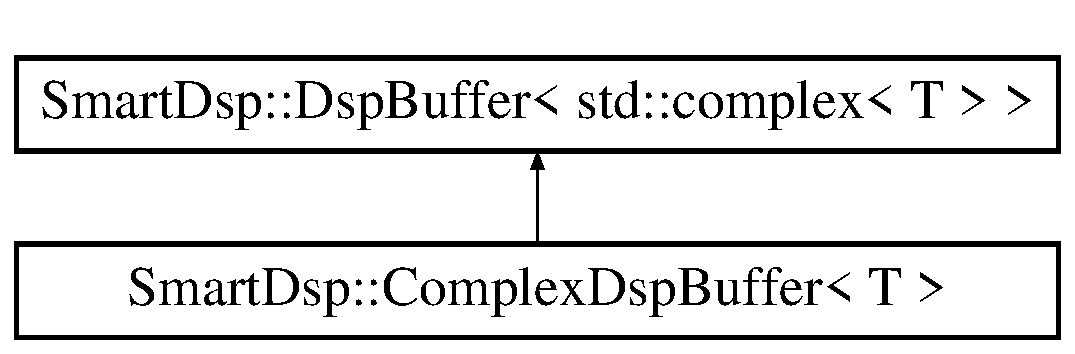
\includegraphics[height=2.000000cm]{class_smart_dsp_1_1_complex_dsp_buffer}
\end{center}
\end{figure}
\subsection*{Public Member Functions}
\begin{DoxyCompactItemize}
\item 
\hyperlink{class_smart_dsp_1_1_complex_dsp_buffer_abf8205d2b2da2719ec01f5a42928c02a}{Complex\+Dsp\+Buffer} (void)
\item 
\hyperlink{class_smart_dsp_1_1_complex_dsp_buffer_a6491f355dc36aff799b7518444be907e}{Complex\+Dsp\+Buffer} (unsigned \hyperlink{class_smart_dsp_1_1_dsp_buffer_af931c57c26c1f459cae47ca4b249d402}{size})
\item 
{\footnotesize template$<$typename U $>$ }\\\hyperlink{class_smart_dsp_1_1_complex_dsp_buffer_a7bb259898457e3cd449143264e3d948c}{Complex\+Dsp\+Buffer} (std\+::vector$<$ U $>$ data, \hyperlink{namespace_smart_dsp_a0aa2e95fc5daec3aee23af9976fcafa5}{Domain\+Type} data\+Domain=\hyperlink{namespace_smart_dsp_a0aa2e95fc5daec3aee23af9976fcafa5aeb7171be8bf3e58d9181dfb17a37b05f}{T\+I\+M\+E\+\_\+\+D\+O\+M\+A\+I\+N})
\item 
{\footnotesize template$<$typename U $>$ }\\\hyperlink{class_smart_dsp_1_1_complex_dsp_buffer_a0fe2d55b5d9b5f2871bd5dc3ed6efe93}{Complex\+Dsp\+Buffer} (U $\ast$data, unsigned data\+Len, \hyperlink{namespace_smart_dsp_a0aa2e95fc5daec3aee23af9976fcafa5}{Domain\+Type} data\+Domain=\hyperlink{namespace_smart_dsp_a0aa2e95fc5daec3aee23af9976fcafa5aeb7171be8bf3e58d9181dfb17a37b05f}{T\+I\+M\+E\+\_\+\+D\+O\+M\+A\+I\+N})
\item 
\hyperlink{class_smart_dsp_1_1_complex_dsp_buffer_a7f178a71d2e145a4adcd2e8ae43ffc95}{Complex\+Dsp\+Buffer} (const \hyperlink{class_smart_dsp_1_1_complex_dsp_buffer}{Complex\+Dsp\+Buffer}$<$ T $>$ \&other)
\item 
\hyperlink{class_smart_dsp_1_1_complex_dsp_buffer}{Complex\+Dsp\+Buffer}$<$ T $>$ \& \hyperlink{class_smart_dsp_1_1_complex_dsp_buffer_a0c760c221731beb2a9420e5f4a78459b}{operator=} (const \hyperlink{class_smart_dsp_1_1_complex_dsp_buffer}{Complex\+Dsp\+Buffer}$<$ T $>$ \&rhs)
\item 
\hyperlink{class_smart_dsp_1_1_complex_dsp_buffer}{Complex\+Dsp\+Buffer}$<$ T $>$ \& \hyperlink{class_smart_dsp_1_1_complex_dsp_buffer_a2f81014300646ede5b3375dae6336eaa}{operator=} (const \hyperlink{class_smart_dsp_1_1_dsp_buffer}{Dsp\+Buffer}$<$ std\+::complex$<$ T $>$ $>$ \&rhs)
\item 
\hyperlink{class_smart_dsp_1_1_complex_dsp_buffer}{Complex\+Dsp\+Buffer}$<$ T $>$ \& \hyperlink{class_smart_dsp_1_1_complex_dsp_buffer_aec4366235f3edf309de92965935b78cd}{pow} (const std\+::complex$<$ \hyperlink{_dsp_buffer_8h_a9ed4123d332590f7a6161bc2061eac49}{S\+M\+A\+R\+T\+D\+S\+P\+\_\+\+F\+L\+O\+A\+T\+\_\+\+T\+Y\+P\+E} $>$ \&exponent)
\item 
const std\+::complex\\*
$<$ \hyperlink{_dsp_buffer_8h_a9ed4123d332590f7a6161bc2061eac49}{S\+M\+A\+R\+T\+D\+S\+P\+\_\+\+F\+L\+O\+A\+T\+\_\+\+T\+Y\+P\+E} $>$ \hyperlink{class_smart_dsp_1_1_complex_dsp_buffer_a7da9f78136a95bec50655db8691dfb0a}{mean} () const 
\item 
const \hyperlink{_dsp_buffer_8h_a9ed4123d332590f7a6161bc2061eac49}{S\+M\+A\+R\+T\+D\+S\+P\+\_\+\+F\+L\+O\+A\+T\+\_\+\+T\+Y\+P\+E} \hyperlink{class_smart_dsp_1_1_complex_dsp_buffer_af78c489f4a00ae0b8d5fa5d64feb7abc}{var} () const 
\item 
const \hyperlink{_dsp_buffer_8h_a9ed4123d332590f7a6161bc2061eac49}{S\+M\+A\+R\+T\+D\+S\+P\+\_\+\+F\+L\+O\+A\+T\+\_\+\+T\+Y\+P\+E} \hyperlink{class_smart_dsp_1_1_complex_dsp_buffer_a716333b41953cf8819d0eec56aa46586}{std\+Dev} () const 
\item 
\hyperlink{class_smart_dsp_1_1_complex_dsp_buffer}{Complex\+Dsp\+Buffer}$<$ T $>$ \& \hyperlink{class_smart_dsp_1_1_complex_dsp_buffer_afbef620dde7dad4d74bde4f5c1b9dea7}{saturate} (const std\+::complex$<$ T $>$ \&val)
\item 
\hyperlink{class_smart_dsp_1_1_complex_dsp_buffer}{Complex\+Dsp\+Buffer}$<$ T $>$ \& \hyperlink{class_smart_dsp_1_1_complex_dsp_buffer_a1e788380918a6f69d3b0108b86e674b7}{conj} ()
\item 
\hyperlink{class_smart_dsp_1_1_complex_dsp_buffer}{Complex\+Dsp\+Buffer}$<$ T $>$ \& \hyperlink{class_smart_dsp_1_1_complex_dsp_buffer_a47e61137f6dbce0f011ba646b573be7a}{mag\+Sq} ()
\item 
\hyperlink{class_smart_dsp_1_1_complex_dsp_buffer}{Complex\+Dsp\+Buffer}$<$ T $>$ \& \hyperlink{class_smart_dsp_1_1_complex_dsp_buffer_a0b113e3c71f99cdda46fb1d9f68cf7f4}{angle} ()
\item 
\hyperlink{class_smart_dsp_1_1_complex_dsp_buffer}{Complex\+Dsp\+Buffer}$<$ T $>$ \& \hyperlink{class_smart_dsp_1_1_complex_dsp_buffer_a17a6c426c513f4bb0a71ee537d7407a3}{fft} ()
\item 
\hyperlink{class_smart_dsp_1_1_complex_dsp_buffer}{Complex\+Dsp\+Buffer}$<$ T $>$ \& \hyperlink{class_smart_dsp_1_1_complex_dsp_buffer_a6eb8421aa0d6ace37d2966b2bce4af24}{ifft} ()
\end{DoxyCompactItemize}
\subsection*{Public Attributes}
\begin{DoxyCompactItemize}
\item 
\hyperlink{namespace_smart_dsp_a0aa2e95fc5daec3aee23af9976fcafa5}{Domain\+Type} \hyperlink{class_smart_dsp_1_1_complex_dsp_buffer_ab4954544b54bb7bd220c66f979d294b2}{domain}
\end{DoxyCompactItemize}
\subsection*{Additional Inherited Members}


\subsection{Detailed Description}
\subsubsection*{template$<$class T$>$class Smart\+Dsp\+::\+Complex\+Dsp\+Buffer$<$ T $>$}



Definition at line 24 of file Complex\+Dsp\+Buffer.\+h.



\subsection{Constructor \& Destructor Documentation}
\hypertarget{class_smart_dsp_1_1_complex_dsp_buffer_abf8205d2b2da2719ec01f5a42928c02a}{\index{Smart\+Dsp\+::\+Complex\+Dsp\+Buffer@{Smart\+Dsp\+::\+Complex\+Dsp\+Buffer}!Complex\+Dsp\+Buffer@{Complex\+Dsp\+Buffer}}
\index{Complex\+Dsp\+Buffer@{Complex\+Dsp\+Buffer}!Smart\+Dsp\+::\+Complex\+Dsp\+Buffer@{Smart\+Dsp\+::\+Complex\+Dsp\+Buffer}}
\subsubsection[{Complex\+Dsp\+Buffer}]{\setlength{\rightskip}{0pt plus 5cm}template$<$class T$>$ {\bf Smart\+Dsp\+::\+Complex\+Dsp\+Buffer}$<$ T $>$\+::{\bf Complex\+Dsp\+Buffer} (
\begin{DoxyParamCaption}
\item[{void}]{}
\end{DoxyParamCaption}
)\hspace{0.3cm}{\ttfamily [inline]}}}\label{class_smart_dsp_1_1_complex_dsp_buffer_abf8205d2b2da2719ec01f5a42928c02a}


Definition at line 29 of file Complex\+Dsp\+Buffer.\+h.

\hypertarget{class_smart_dsp_1_1_complex_dsp_buffer_a6491f355dc36aff799b7518444be907e}{\index{Smart\+Dsp\+::\+Complex\+Dsp\+Buffer@{Smart\+Dsp\+::\+Complex\+Dsp\+Buffer}!Complex\+Dsp\+Buffer@{Complex\+Dsp\+Buffer}}
\index{Complex\+Dsp\+Buffer@{Complex\+Dsp\+Buffer}!Smart\+Dsp\+::\+Complex\+Dsp\+Buffer@{Smart\+Dsp\+::\+Complex\+Dsp\+Buffer}}
\subsubsection[{Complex\+Dsp\+Buffer}]{\setlength{\rightskip}{0pt plus 5cm}template$<$class T$>$ {\bf Smart\+Dsp\+::\+Complex\+Dsp\+Buffer}$<$ T $>$\+::{\bf Complex\+Dsp\+Buffer} (
\begin{DoxyParamCaption}
\item[{unsigned}]{size}
\end{DoxyParamCaption}
)\hspace{0.3cm}{\ttfamily [inline]}}}\label{class_smart_dsp_1_1_complex_dsp_buffer_a6491f355dc36aff799b7518444be907e}


Definition at line 30 of file Complex\+Dsp\+Buffer.\+h.

\hypertarget{class_smart_dsp_1_1_complex_dsp_buffer_a7bb259898457e3cd449143264e3d948c}{\index{Smart\+Dsp\+::\+Complex\+Dsp\+Buffer@{Smart\+Dsp\+::\+Complex\+Dsp\+Buffer}!Complex\+Dsp\+Buffer@{Complex\+Dsp\+Buffer}}
\index{Complex\+Dsp\+Buffer@{Complex\+Dsp\+Buffer}!Smart\+Dsp\+::\+Complex\+Dsp\+Buffer@{Smart\+Dsp\+::\+Complex\+Dsp\+Buffer}}
\subsubsection[{Complex\+Dsp\+Buffer}]{\setlength{\rightskip}{0pt plus 5cm}template$<$class T$>$ template$<$typename U $>$ {\bf Smart\+Dsp\+::\+Complex\+Dsp\+Buffer}$<$ T $>$\+::{\bf Complex\+Dsp\+Buffer} (
\begin{DoxyParamCaption}
\item[{std\+::vector$<$ U $>$}]{data, }
\item[{{\bf Domain\+Type}}]{data\+Domain = {\ttfamily {\bf T\+I\+M\+E\+\_\+\+D\+O\+M\+A\+I\+N}}}
\end{DoxyParamCaption}
)\hspace{0.3cm}{\ttfamily [inline]}}}\label{class_smart_dsp_1_1_complex_dsp_buffer_a7bb259898457e3cd449143264e3d948c}


Definition at line 32 of file Complex\+Dsp\+Buffer.\+h.

\hypertarget{class_smart_dsp_1_1_complex_dsp_buffer_a0fe2d55b5d9b5f2871bd5dc3ed6efe93}{\index{Smart\+Dsp\+::\+Complex\+Dsp\+Buffer@{Smart\+Dsp\+::\+Complex\+Dsp\+Buffer}!Complex\+Dsp\+Buffer@{Complex\+Dsp\+Buffer}}
\index{Complex\+Dsp\+Buffer@{Complex\+Dsp\+Buffer}!Smart\+Dsp\+::\+Complex\+Dsp\+Buffer@{Smart\+Dsp\+::\+Complex\+Dsp\+Buffer}}
\subsubsection[{Complex\+Dsp\+Buffer}]{\setlength{\rightskip}{0pt plus 5cm}template$<$class T$>$ template$<$typename U $>$ {\bf Smart\+Dsp\+::\+Complex\+Dsp\+Buffer}$<$ T $>$\+::{\bf Complex\+Dsp\+Buffer} (
\begin{DoxyParamCaption}
\item[{U $\ast$}]{data, }
\item[{unsigned}]{data\+Len, }
\item[{{\bf Domain\+Type}}]{data\+Domain = {\ttfamily {\bf T\+I\+M\+E\+\_\+\+D\+O\+M\+A\+I\+N}}}
\end{DoxyParamCaption}
)\hspace{0.3cm}{\ttfamily [inline]}}}\label{class_smart_dsp_1_1_complex_dsp_buffer_a0fe2d55b5d9b5f2871bd5dc3ed6efe93}


Definition at line 34 of file Complex\+Dsp\+Buffer.\+h.

\hypertarget{class_smart_dsp_1_1_complex_dsp_buffer_a7f178a71d2e145a4adcd2e8ae43ffc95}{\index{Smart\+Dsp\+::\+Complex\+Dsp\+Buffer@{Smart\+Dsp\+::\+Complex\+Dsp\+Buffer}!Complex\+Dsp\+Buffer@{Complex\+Dsp\+Buffer}}
\index{Complex\+Dsp\+Buffer@{Complex\+Dsp\+Buffer}!Smart\+Dsp\+::\+Complex\+Dsp\+Buffer@{Smart\+Dsp\+::\+Complex\+Dsp\+Buffer}}
\subsubsection[{Complex\+Dsp\+Buffer}]{\setlength{\rightskip}{0pt plus 5cm}template$<$class T$>$ {\bf Smart\+Dsp\+::\+Complex\+Dsp\+Buffer}$<$ T $>$\+::{\bf Complex\+Dsp\+Buffer} (
\begin{DoxyParamCaption}
\item[{const {\bf Complex\+Dsp\+Buffer}$<$ T $>$ \&}]{other}
\end{DoxyParamCaption}
)\hspace{0.3cm}{\ttfamily [inline]}}}\label{class_smart_dsp_1_1_complex_dsp_buffer_a7f178a71d2e145a4adcd2e8ae43ffc95}


Definition at line 36 of file Complex\+Dsp\+Buffer.\+h.



\subsection{Member Function Documentation}
\hypertarget{class_smart_dsp_1_1_complex_dsp_buffer_a0b113e3c71f99cdda46fb1d9f68cf7f4}{\index{Smart\+Dsp\+::\+Complex\+Dsp\+Buffer@{Smart\+Dsp\+::\+Complex\+Dsp\+Buffer}!angle@{angle}}
\index{angle@{angle}!Smart\+Dsp\+::\+Complex\+Dsp\+Buffer@{Smart\+Dsp\+::\+Complex\+Dsp\+Buffer}}
\subsubsection[{angle}]{\setlength{\rightskip}{0pt plus 5cm}template$<$class T $>$ {\bf Complex\+Dsp\+Buffer}$<$ T $>$ \& {\bf Smart\+Dsp\+::\+Complex\+Dsp\+Buffer}$<$ T $>$\+::angle (
\begin{DoxyParamCaption}
{}
\end{DoxyParamCaption}
)}}\label{class_smart_dsp_1_1_complex_dsp_buffer_a0b113e3c71f99cdda46fb1d9f68cf7f4}


Definition at line 207 of file Complex\+Dsp\+Buffer.\+h.

\hypertarget{class_smart_dsp_1_1_complex_dsp_buffer_a1e788380918a6f69d3b0108b86e674b7}{\index{Smart\+Dsp\+::\+Complex\+Dsp\+Buffer@{Smart\+Dsp\+::\+Complex\+Dsp\+Buffer}!conj@{conj}}
\index{conj@{conj}!Smart\+Dsp\+::\+Complex\+Dsp\+Buffer@{Smart\+Dsp\+::\+Complex\+Dsp\+Buffer}}
\subsubsection[{conj}]{\setlength{\rightskip}{0pt plus 5cm}template$<$class T $>$ {\bf Complex\+Dsp\+Buffer}$<$ T $>$ \& {\bf Smart\+Dsp\+::\+Complex\+Dsp\+Buffer}$<$ T $>$\+::conj (
\begin{DoxyParamCaption}
{}
\end{DoxyParamCaption}
)}}\label{class_smart_dsp_1_1_complex_dsp_buffer_a1e788380918a6f69d3b0108b86e674b7}


Definition at line 157 of file Complex\+Dsp\+Buffer.\+h.

\hypertarget{class_smart_dsp_1_1_complex_dsp_buffer_a17a6c426c513f4bb0a71ee537d7407a3}{\index{Smart\+Dsp\+::\+Complex\+Dsp\+Buffer@{Smart\+Dsp\+::\+Complex\+Dsp\+Buffer}!fft@{fft}}
\index{fft@{fft}!Smart\+Dsp\+::\+Complex\+Dsp\+Buffer@{Smart\+Dsp\+::\+Complex\+Dsp\+Buffer}}
\subsubsection[{fft}]{\setlength{\rightskip}{0pt plus 5cm}template$<$class T $>$ {\bf Complex\+Dsp\+Buffer}$<$ T $>$ \& {\bf Smart\+Dsp\+::\+Complex\+Dsp\+Buffer}$<$ T $>$\+::fft (
\begin{DoxyParamCaption}
{}
\end{DoxyParamCaption}
)}}\label{class_smart_dsp_1_1_complex_dsp_buffer_a17a6c426c513f4bb0a71ee537d7407a3}


Definition at line 139 of file Complex\+Dsp\+Buffer.\+h.

\hypertarget{class_smart_dsp_1_1_complex_dsp_buffer_a6eb8421aa0d6ace37d2966b2bce4af24}{\index{Smart\+Dsp\+::\+Complex\+Dsp\+Buffer@{Smart\+Dsp\+::\+Complex\+Dsp\+Buffer}!ifft@{ifft}}
\index{ifft@{ifft}!Smart\+Dsp\+::\+Complex\+Dsp\+Buffer@{Smart\+Dsp\+::\+Complex\+Dsp\+Buffer}}
\subsubsection[{ifft}]{\setlength{\rightskip}{0pt plus 5cm}template$<$class T $>$ {\bf Complex\+Dsp\+Buffer}$<$ T $>$ \& {\bf Smart\+Dsp\+::\+Complex\+Dsp\+Buffer}$<$ T $>$\+::ifft (
\begin{DoxyParamCaption}
{}
\end{DoxyParamCaption}
)}}\label{class_smart_dsp_1_1_complex_dsp_buffer_a6eb8421aa0d6ace37d2966b2bce4af24}


Definition at line 189 of file Complex\+Dsp\+Buffer.\+h.

\hypertarget{class_smart_dsp_1_1_complex_dsp_buffer_a47e61137f6dbce0f011ba646b573be7a}{\index{Smart\+Dsp\+::\+Complex\+Dsp\+Buffer@{Smart\+Dsp\+::\+Complex\+Dsp\+Buffer}!mag\+Sq@{mag\+Sq}}
\index{mag\+Sq@{mag\+Sq}!Smart\+Dsp\+::\+Complex\+Dsp\+Buffer@{Smart\+Dsp\+::\+Complex\+Dsp\+Buffer}}
\subsubsection[{mag\+Sq}]{\setlength{\rightskip}{0pt plus 5cm}template$<$class T $>$ {\bf Complex\+Dsp\+Buffer}$<$ T $>$ \& {\bf Smart\+Dsp\+::\+Complex\+Dsp\+Buffer}$<$ T $>$\+::mag\+Sq (
\begin{DoxyParamCaption}
{}
\end{DoxyParamCaption}
)}}\label{class_smart_dsp_1_1_complex_dsp_buffer_a47e61137f6dbce0f011ba646b573be7a}


Definition at line 175 of file Complex\+Dsp\+Buffer.\+h.

\hypertarget{class_smart_dsp_1_1_complex_dsp_buffer_a7da9f78136a95bec50655db8691dfb0a}{\index{Smart\+Dsp\+::\+Complex\+Dsp\+Buffer@{Smart\+Dsp\+::\+Complex\+Dsp\+Buffer}!mean@{mean}}
\index{mean@{mean}!Smart\+Dsp\+::\+Complex\+Dsp\+Buffer@{Smart\+Dsp\+::\+Complex\+Dsp\+Buffer}}
\subsubsection[{mean}]{\setlength{\rightskip}{0pt plus 5cm}template$<$class T $>$ const std\+::complex$<$ {\bf S\+M\+A\+R\+T\+D\+S\+P\+\_\+\+F\+L\+O\+A\+T\+\_\+\+T\+Y\+P\+E} $>$ {\bf Smart\+Dsp\+::\+Complex\+Dsp\+Buffer}$<$ T $>$\+::mean (
\begin{DoxyParamCaption}
{}
\end{DoxyParamCaption}
) const}}\label{class_smart_dsp_1_1_complex_dsp_buffer_a7da9f78136a95bec50655db8691dfb0a}


Definition at line 87 of file Complex\+Dsp\+Buffer.\+h.

\hypertarget{class_smart_dsp_1_1_complex_dsp_buffer_a0c760c221731beb2a9420e5f4a78459b}{\index{Smart\+Dsp\+::\+Complex\+Dsp\+Buffer@{Smart\+Dsp\+::\+Complex\+Dsp\+Buffer}!operator=@{operator=}}
\index{operator=@{operator=}!Smart\+Dsp\+::\+Complex\+Dsp\+Buffer@{Smart\+Dsp\+::\+Complex\+Dsp\+Buffer}}
\subsubsection[{operator=}]{\setlength{\rightskip}{0pt plus 5cm}template$<$class T $>$ {\bf Complex\+Dsp\+Buffer}$<$ T $>$ \& {\bf Smart\+Dsp\+::\+Complex\+Dsp\+Buffer}$<$ T $>$\+::operator= (
\begin{DoxyParamCaption}
\item[{const {\bf Complex\+Dsp\+Buffer}$<$ T $>$ \&}]{rhs}
\end{DoxyParamCaption}
)}}\label{class_smart_dsp_1_1_complex_dsp_buffer_a0c760c221731beb2a9420e5f4a78459b}


Definition at line 58 of file Complex\+Dsp\+Buffer.\+h.

\hypertarget{class_smart_dsp_1_1_complex_dsp_buffer_a2f81014300646ede5b3375dae6336eaa}{\index{Smart\+Dsp\+::\+Complex\+Dsp\+Buffer@{Smart\+Dsp\+::\+Complex\+Dsp\+Buffer}!operator=@{operator=}}
\index{operator=@{operator=}!Smart\+Dsp\+::\+Complex\+Dsp\+Buffer@{Smart\+Dsp\+::\+Complex\+Dsp\+Buffer}}
\subsubsection[{operator=}]{\setlength{\rightskip}{0pt plus 5cm}template$<$class T $>$ {\bf Complex\+Dsp\+Buffer}$<$ T $>$ \& {\bf Smart\+Dsp\+::\+Complex\+Dsp\+Buffer}$<$ T $>$\+::operator= (
\begin{DoxyParamCaption}
\item[{const {\bf Dsp\+Buffer}$<$ std\+::complex$<$ T $>$ $>$ \&}]{rhs}
\end{DoxyParamCaption}
)}}\label{class_smart_dsp_1_1_complex_dsp_buffer_a2f81014300646ede5b3375dae6336eaa}


Definition at line 66 of file Complex\+Dsp\+Buffer.\+h.

\hypertarget{class_smart_dsp_1_1_complex_dsp_buffer_aec4366235f3edf309de92965935b78cd}{\index{Smart\+Dsp\+::\+Complex\+Dsp\+Buffer@{Smart\+Dsp\+::\+Complex\+Dsp\+Buffer}!pow@{pow}}
\index{pow@{pow}!Smart\+Dsp\+::\+Complex\+Dsp\+Buffer@{Smart\+Dsp\+::\+Complex\+Dsp\+Buffer}}
\subsubsection[{pow}]{\setlength{\rightskip}{0pt plus 5cm}template$<$class T $>$ {\bf Complex\+Dsp\+Buffer}$<$ T $>$ \& {\bf Smart\+Dsp\+::\+Complex\+Dsp\+Buffer}$<$ T $>$\+::pow (
\begin{DoxyParamCaption}
\item[{const std\+::complex$<$ {\bf S\+M\+A\+R\+T\+D\+S\+P\+\_\+\+F\+L\+O\+A\+T\+\_\+\+T\+Y\+P\+E} $>$ \&}]{exponent}
\end{DoxyParamCaption}
)}}\label{class_smart_dsp_1_1_complex_dsp_buffer_aec4366235f3edf309de92965935b78cd}


Definition at line 74 of file Complex\+Dsp\+Buffer.\+h.

\hypertarget{class_smart_dsp_1_1_complex_dsp_buffer_afbef620dde7dad4d74bde4f5c1b9dea7}{\index{Smart\+Dsp\+::\+Complex\+Dsp\+Buffer@{Smart\+Dsp\+::\+Complex\+Dsp\+Buffer}!saturate@{saturate}}
\index{saturate@{saturate}!Smart\+Dsp\+::\+Complex\+Dsp\+Buffer@{Smart\+Dsp\+::\+Complex\+Dsp\+Buffer}}
\subsubsection[{saturate}]{\setlength{\rightskip}{0pt plus 5cm}template$<$class T $>$ {\bf Complex\+Dsp\+Buffer}$<$ T $>$ \& {\bf Smart\+Dsp\+::\+Complex\+Dsp\+Buffer}$<$ T $>$\+::saturate (
\begin{DoxyParamCaption}
\item[{const std\+::complex$<$ T $>$ \&}]{val}
\end{DoxyParamCaption}
)}}\label{class_smart_dsp_1_1_complex_dsp_buffer_afbef620dde7dad4d74bde4f5c1b9dea7}


Definition at line 124 of file Complex\+Dsp\+Buffer.\+h.

\hypertarget{class_smart_dsp_1_1_complex_dsp_buffer_a716333b41953cf8819d0eec56aa46586}{\index{Smart\+Dsp\+::\+Complex\+Dsp\+Buffer@{Smart\+Dsp\+::\+Complex\+Dsp\+Buffer}!std\+Dev@{std\+Dev}}
\index{std\+Dev@{std\+Dev}!Smart\+Dsp\+::\+Complex\+Dsp\+Buffer@{Smart\+Dsp\+::\+Complex\+Dsp\+Buffer}}
\subsubsection[{std\+Dev}]{\setlength{\rightskip}{0pt plus 5cm}template$<$class T$>$ const {\bf S\+M\+A\+R\+T\+D\+S\+P\+\_\+\+F\+L\+O\+A\+T\+\_\+\+T\+Y\+P\+E} {\bf Smart\+Dsp\+::\+Complex\+Dsp\+Buffer}$<$ T $>$\+::std\+Dev (
\begin{DoxyParamCaption}
{}
\end{DoxyParamCaption}
) const\hspace{0.3cm}{\ttfamily [inline]}}}\label{class_smart_dsp_1_1_complex_dsp_buffer_a716333b41953cf8819d0eec56aa46586}


Definition at line 45 of file Complex\+Dsp\+Buffer.\+h.

\hypertarget{class_smart_dsp_1_1_complex_dsp_buffer_af78c489f4a00ae0b8d5fa5d64feb7abc}{\index{Smart\+Dsp\+::\+Complex\+Dsp\+Buffer@{Smart\+Dsp\+::\+Complex\+Dsp\+Buffer}!var@{var}}
\index{var@{var}!Smart\+Dsp\+::\+Complex\+Dsp\+Buffer@{Smart\+Dsp\+::\+Complex\+Dsp\+Buffer}}
\subsubsection[{var}]{\setlength{\rightskip}{0pt plus 5cm}template$<$class T $>$ const {\bf S\+M\+A\+R\+T\+D\+S\+P\+\_\+\+F\+L\+O\+A\+T\+\_\+\+T\+Y\+P\+E} {\bf Smart\+Dsp\+::\+Complex\+Dsp\+Buffer}$<$ T $>$\+::var (
\begin{DoxyParamCaption}
{}
\end{DoxyParamCaption}
) const}}\label{class_smart_dsp_1_1_complex_dsp_buffer_af78c489f4a00ae0b8d5fa5d64feb7abc}


Definition at line 102 of file Complex\+Dsp\+Buffer.\+h.



\subsection{Member Data Documentation}
\hypertarget{class_smart_dsp_1_1_complex_dsp_buffer_ab4954544b54bb7bd220c66f979d294b2}{\index{Smart\+Dsp\+::\+Complex\+Dsp\+Buffer@{Smart\+Dsp\+::\+Complex\+Dsp\+Buffer}!domain@{domain}}
\index{domain@{domain}!Smart\+Dsp\+::\+Complex\+Dsp\+Buffer@{Smart\+Dsp\+::\+Complex\+Dsp\+Buffer}}
\subsubsection[{domain}]{\setlength{\rightskip}{0pt plus 5cm}template$<$class T$>$ {\bf Domain\+Type} {\bf Smart\+Dsp\+::\+Complex\+Dsp\+Buffer}$<$ T $>$\+::domain}}\label{class_smart_dsp_1_1_complex_dsp_buffer_ab4954544b54bb7bd220c66f979d294b2}


Definition at line 26 of file Complex\+Dsp\+Buffer.\+h.



The documentation for this class was generated from the following file\+:\begin{DoxyCompactItemize}
\item 
src/\hyperlink{_complex_dsp_buffer_8h}{Complex\+Dsp\+Buffer.\+h}\end{DoxyCompactItemize}

\hypertarget{class_smart_dsp_1_1_dsp_buffer}{\section{Smart\+Dsp\+:\+:Dsp\+Buffer$<$ T $>$ Class Template Reference}
\label{class_smart_dsp_1_1_dsp_buffer}\index{Smart\+Dsp\+::\+Dsp\+Buffer$<$ T $>$@{Smart\+Dsp\+::\+Dsp\+Buffer$<$ T $>$}}
}


Base class for \hyperlink{namespace_smart_dsp}{Smart\+Dsp}.  




{\ttfamily \#include $<$Dsp\+Buffer.\+h$>$}

Inheritance diagram for Smart\+Dsp\+:\+:Dsp\+Buffer$<$ T $>$\+:\begin{figure}[H]
\begin{center}
\leavevmode
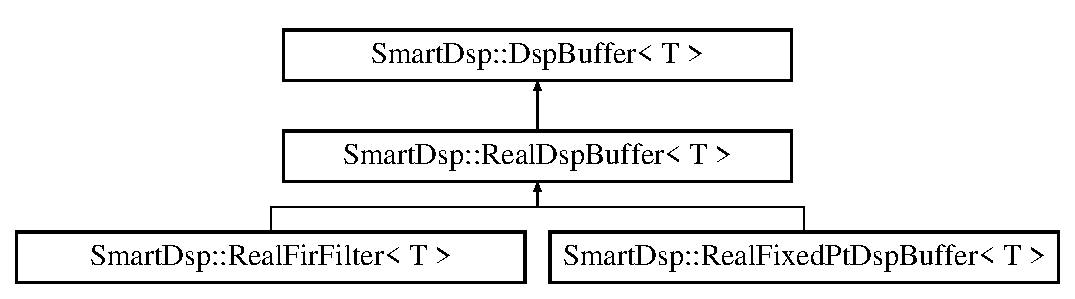
\includegraphics[height=3.000000cm]{class_smart_dsp_1_1_dsp_buffer}
\end{center}
\end{figure}
\subsection*{Public Member Functions}
\begin{DoxyCompactItemize}
\item 
\hyperlink{class_smart_dsp_1_1_dsp_buffer_aac9cefffb64fddbc22575b5592106566}{Dsp\+Buffer} (unsigned \hyperlink{class_smart_dsp_1_1_dsp_buffer_af931c57c26c1f459cae47ca4b249d402}{size}=0, std\+::vector$<$ T $>$ $\ast$scratch=N\+U\+L\+L)
\begin{DoxyCompactList}\small\item\em Basic constructor. \end{DoxyCompactList}\item 
{\footnotesize template$<$typename U $>$ }\\\hyperlink{class_smart_dsp_1_1_dsp_buffer_aeacaa5323f91a1c1a38ba1cc0b66f154}{Dsp\+Buffer} (std\+::vector$<$ U $>$ data, std\+::vector$<$ T $>$ $\ast$scratch=N\+U\+L\+L)
\begin{DoxyCompactList}\small\item\em Vector constructor. \end{DoxyCompactList}\item 
{\footnotesize template$<$typename U $>$ }\\\hyperlink{class_smart_dsp_1_1_dsp_buffer_a97d1b8eeeef8b83d3d5197ea8f9c14fd}{Dsp\+Buffer} (U $\ast$data, unsigned data\+Len, std\+::vector$<$ T $>$ $\ast$scratch=N\+U\+L\+L)
\begin{DoxyCompactList}\small\item\em Array constructor. \end{DoxyCompactList}\item 
\hyperlink{class_smart_dsp_1_1_dsp_buffer_a8bf1ba415d8ace450b3c6a241165c545}{Dsp\+Buffer} (const \hyperlink{class_smart_dsp_1_1_dsp_buffer}{Dsp\+Buffer}$<$ T $>$ \&other)
\begin{DoxyCompactList}\small\item\em Copy constructor. \end{DoxyCompactList}\item 
\hyperlink{class_smart_dsp_1_1_dsp_buffer}{Dsp\+Buffer}$<$ T $>$ \& \hyperlink{class_smart_dsp_1_1_dsp_buffer_aefbe05ec4f15746bef8086b75be69f18}{operator=} (const \hyperlink{class_smart_dsp_1_1_dsp_buffer}{Dsp\+Buffer}$<$ T $>$ \&rhs)
\begin{DoxyCompactList}\small\item\em Assignment operator. \end{DoxyCompactList}\item 
\hyperlink{class_smart_dsp_1_1_dsp_buffer}{Dsp\+Buffer}$<$ T $>$ \& \hyperlink{class_smart_dsp_1_1_dsp_buffer_a808b7f21c55dac554a5499f909b99ee7}{operator-\/} ()
\begin{DoxyCompactList}\small\item\em Unary minus (negation) operator. \end{DoxyCompactList}\item 
{\footnotesize template$<$class U $>$ }\\\hyperlink{class_smart_dsp_1_1_dsp_buffer}{Dsp\+Buffer}$<$ T $>$ \& \hyperlink{class_smart_dsp_1_1_dsp_buffer_a1f82292301361be32e2b8ac8521aa22b}{operator+=} (const \hyperlink{class_smart_dsp_1_1_dsp_buffer}{Dsp\+Buffer}$<$ U $>$ \&rhs)
\begin{DoxyCompactList}\small\item\em Add Buffer/\+Assignment operator. \end{DoxyCompactList}\item 
\hyperlink{class_smart_dsp_1_1_dsp_buffer}{Dsp\+Buffer}$<$ T $>$ \& \hyperlink{class_smart_dsp_1_1_dsp_buffer_a3ea52379f390c48af5db2cc19f9555d2}{operator+=} (const T \&rhs)
\begin{DoxyCompactList}\small\item\em Add Scalar/\+Assignment operator. \end{DoxyCompactList}\item 
{\footnotesize template$<$class U $>$ }\\\hyperlink{class_smart_dsp_1_1_dsp_buffer}{Dsp\+Buffer}$<$ T $>$ \& \hyperlink{class_smart_dsp_1_1_dsp_buffer_ad69dc68623269e99dc24debad52bfa43}{operator-\/=} (const \hyperlink{class_smart_dsp_1_1_dsp_buffer}{Dsp\+Buffer}$<$ U $>$ \&rhs)
\begin{DoxyCompactList}\small\item\em Subtract Buffer/\+Assignment operator. \end{DoxyCompactList}\item 
\hyperlink{class_smart_dsp_1_1_dsp_buffer}{Dsp\+Buffer}$<$ T $>$ \& \hyperlink{class_smart_dsp_1_1_dsp_buffer_aee029f41878033fe1072759a1b1f90e5}{operator-\/=} (const T \&rhs)
\begin{DoxyCompactList}\small\item\em Subtract Scalar/\+Assignment operator. \end{DoxyCompactList}\item 
{\footnotesize template$<$class U $>$ }\\\hyperlink{class_smart_dsp_1_1_dsp_buffer}{Dsp\+Buffer}$<$ T $>$ \& \hyperlink{class_smart_dsp_1_1_dsp_buffer_a6e5da9f656e0d3f3ed986c1c42db8754}{operator$\ast$=} (const \hyperlink{class_smart_dsp_1_1_dsp_buffer}{Dsp\+Buffer}$<$ U $>$ \&rhs)
\begin{DoxyCompactList}\small\item\em Multiply Buffer/\+Assignment operator. \end{DoxyCompactList}\item 
\hyperlink{class_smart_dsp_1_1_dsp_buffer}{Dsp\+Buffer}$<$ T $>$ \& \hyperlink{class_smart_dsp_1_1_dsp_buffer_a71344eecfd0e50516970640eb8aa21b3}{operator$\ast$=} (const T \&rhs)
\begin{DoxyCompactList}\small\item\em Multiply Scalar/\+Assignment operator. \end{DoxyCompactList}\item 
{\footnotesize template$<$class U $>$ }\\\hyperlink{class_smart_dsp_1_1_dsp_buffer}{Dsp\+Buffer}$<$ T $>$ \& \hyperlink{class_smart_dsp_1_1_dsp_buffer_adda7d64b126cce6f49519c4a1ec4dbfd}{operator/=} (const \hyperlink{class_smart_dsp_1_1_dsp_buffer}{Dsp\+Buffer}$<$ U $>$ \&rhs)
\begin{DoxyCompactList}\small\item\em Divide Buffer/\+Assignment operator. \end{DoxyCompactList}\item 
\hyperlink{class_smart_dsp_1_1_dsp_buffer}{Dsp\+Buffer}$<$ T $>$ \& \hyperlink{class_smart_dsp_1_1_dsp_buffer_a32633ee6a77ff31988e4cddd09dd1b88}{operator/=} (const T \&rhs)
\begin{DoxyCompactList}\small\item\em Divide Scalar/\+Assignment operator. \end{DoxyCompactList}\item 
T \& \hyperlink{class_smart_dsp_1_1_dsp_buffer_acbf2de89d89cdc53cca00e0b8cac75a0}{operator\mbox{[}$\,$\mbox{]}} (unsigned index)
\begin{DoxyCompactList}\small\item\em Index assignment operator. \end{DoxyCompactList}\item 
const T \& \hyperlink{class_smart_dsp_1_1_dsp_buffer_a5a82e83f2575d24d1dcc28961220262b}{operator\mbox{[}$\,$\mbox{]}} (unsigned index) const 
\begin{DoxyCompactList}\small\item\em Index operator. \end{DoxyCompactList}\item 
const unsigned \hyperlink{class_smart_dsp_1_1_dsp_buffer_af931c57c26c1f459cae47ca4b249d402}{size} () const 
\begin{DoxyCompactList}\small\item\em Returns the size of \hyperlink{class_smart_dsp_1_1_dsp_buffer_a7abb8184e08f4c9762f66bc75dcd3a6a}{buf}. \end{DoxyCompactList}\item 
\hyperlink{class_smart_dsp_1_1_dsp_buffer}{Dsp\+Buffer}$<$ T $>$ \& \hyperlink{class_smart_dsp_1_1_dsp_buffer_a1a890ef9ea24235e694573a97217c4eb}{rotate} (int num\+To\+Shift)
\begin{DoxyCompactList}\small\item\em Circular rotation. \end{DoxyCompactList}\item 
\hyperlink{class_smart_dsp_1_1_dsp_buffer}{Dsp\+Buffer}$<$ T $>$ \& \hyperlink{class_smart_dsp_1_1_dsp_buffer_a8f877fbc18d1c64e837e1a9bf7a02bbe}{reverse} ()
\begin{DoxyCompactList}\small\item\em Reverses the order of the elements in \hyperlink{class_smart_dsp_1_1_dsp_buffer_a7abb8184e08f4c9762f66bc75dcd3a6a}{buf}. \end{DoxyCompactList}\item 
const int \hyperlink{class_smart_dsp_1_1_dsp_buffer_a4cbf9ae9ee457bfde36cedbdaf26525c}{find} (const T val) const 
\begin{DoxyCompactList}\small\item\em Finds the first instance of \char`\"{}val\char`\"{} in \hyperlink{class_smart_dsp_1_1_dsp_buffer_a7abb8184e08f4c9762f66bc75dcd3a6a}{buf}. \end{DoxyCompactList}\item 
\hyperlink{class_smart_dsp_1_1_dsp_buffer}{Dsp\+Buffer}$<$ T $>$ \& \hyperlink{class_smart_dsp_1_1_dsp_buffer_a2df860e42f26ca1e261de9228b5a160a}{abs} ()
\begin{DoxyCompactList}\small\item\em Changes the elements of \hyperlink{class_smart_dsp_1_1_dsp_buffer_a7abb8184e08f4c9762f66bc75dcd3a6a}{buf} to their absolute value. \end{DoxyCompactList}\item 
\hyperlink{class_smart_dsp_1_1_dsp_buffer}{Dsp\+Buffer}$<$ T $>$ \& \hyperlink{class_smart_dsp_1_1_dsp_buffer_a0254217926a884db4baccea5d913aef8}{exp} ()
\begin{DoxyCompactList}\small\item\em Sets each element of \hyperlink{class_smart_dsp_1_1_dsp_buffer_a7abb8184e08f4c9762f66bc75dcd3a6a}{buf} to e$^\wedge$(element). \end{DoxyCompactList}\item 
\hyperlink{class_smart_dsp_1_1_dsp_buffer}{Dsp\+Buffer}$<$ T $>$ \& \hyperlink{class_smart_dsp_1_1_dsp_buffer_aecf9005a8cf2502899da5bc25ae1b650}{log} ()
\begin{DoxyCompactList}\small\item\em Sets each element of \hyperlink{class_smart_dsp_1_1_dsp_buffer_a7abb8184e08f4c9762f66bc75dcd3a6a}{buf} to the natural log of the element. \end{DoxyCompactList}\item 
\hyperlink{class_smart_dsp_1_1_dsp_buffer}{Dsp\+Buffer}$<$ T $>$ \& \hyperlink{class_smart_dsp_1_1_dsp_buffer_af9842cde9310511dafeb724d1b82d059}{ln} ()
\begin{DoxyCompactList}\small\item\em Sets each element of \hyperlink{class_smart_dsp_1_1_dsp_buffer_a7abb8184e08f4c9762f66bc75dcd3a6a}{buf} to the natural log of the element. \end{DoxyCompactList}\item 
\hyperlink{class_smart_dsp_1_1_dsp_buffer}{Dsp\+Buffer}$<$ T $>$ \& \hyperlink{class_smart_dsp_1_1_dsp_buffer_ac857bbed4305a0668c5e3960f681ba5d}{log10} ()
\begin{DoxyCompactList}\small\item\em Sets each element of \hyperlink{class_smart_dsp_1_1_dsp_buffer_a7abb8184e08f4c9762f66bc75dcd3a6a}{buf} to the base 10 log of the element. \end{DoxyCompactList}\item 
\hyperlink{class_smart_dsp_1_1_dsp_buffer}{Dsp\+Buffer}$<$ T $>$ \& \hyperlink{class_smart_dsp_1_1_dsp_buffer_af15c581be025d65b1e7934791d27b02e}{resize} (unsigned len, T val=(T) 0)
\begin{DoxyCompactList}\small\item\em Sets the length of \hyperlink{class_smart_dsp_1_1_dsp_buffer_a7abb8184e08f4c9762f66bc75dcd3a6a}{buf} to \char`\"{}len\char`\"{}. \end{DoxyCompactList}\item 
\hyperlink{class_smart_dsp_1_1_dsp_buffer}{Dsp\+Buffer}$<$ T $>$ \& \hyperlink{class_smart_dsp_1_1_dsp_buffer_ae1b10152d9fc0b8fb03bf2fb8d6bdbcd}{pad} (unsigned len, T val=(T) 0)
\begin{DoxyCompactList}\small\item\em Lengthens \hyperlink{class_smart_dsp_1_1_dsp_buffer_a7abb8184e08f4c9762f66bc75dcd3a6a}{buf} by \char`\"{}len\char`\"{} elements. \end{DoxyCompactList}\item 
\hyperlink{class_smart_dsp_1_1_dsp_buffer}{Dsp\+Buffer}$<$ T $>$ \& \hyperlink{class_smart_dsp_1_1_dsp_buffer_ae38a794c1f5e53b6e57b974751345296}{upsample} (int rate, int phase=0)
\begin{DoxyCompactList}\small\item\em Inserts rate-\/1 zeros between samples. \end{DoxyCompactList}\item 
\hyperlink{class_smart_dsp_1_1_dsp_buffer}{Dsp\+Buffer}$<$ T $>$ \& \hyperlink{class_smart_dsp_1_1_dsp_buffer_a75adf718fbcea9f3df132fbb0536ab61}{downsample} (int rate, int phase=0)
\begin{DoxyCompactList}\small\item\em Removes rate-\/1 samples out of every rate samples. \end{DoxyCompactList}\item 
T \hyperlink{class_smart_dsp_1_1_dsp_buffer_af88400d0ec92e4826a364a49ab103433}{sum} () const 
\begin{DoxyCompactList}\small\item\em Returns the sum of all the elements in \hyperlink{class_smart_dsp_1_1_dsp_buffer_a7abb8184e08f4c9762f66bc75dcd3a6a}{buf}. \end{DoxyCompactList}\item 
\hyperlink{class_smart_dsp_1_1_dsp_buffer}{Dsp\+Buffer}$<$ T $>$ \& \hyperlink{class_smart_dsp_1_1_dsp_buffer_a7f9df0331d7e7caafb26c44654f3b07e}{diff} ()
\begin{DoxyCompactList}\small\item\em Replaces \hyperlink{class_smart_dsp_1_1_dsp_buffer_a7abb8184e08f4c9762f66bc75dcd3a6a}{buf} with the difference between successive samples in buf. \end{DoxyCompactList}\item 
\hyperlink{class_smart_dsp_1_1_dsp_buffer}{Dsp\+Buffer}$<$ T $>$ \& \hyperlink{class_smart_dsp_1_1_dsp_buffer_a33d4c84d5be12617fb3230a8ae36cdf9}{diff} (T \&previous\+Val)
\begin{DoxyCompactList}\small\item\em Replaces \hyperlink{class_smart_dsp_1_1_dsp_buffer_a7abb8184e08f4c9762f66bc75dcd3a6a}{buf} with the difference between successive samples in buf. \end{DoxyCompactList}\item 
{\footnotesize template$<$class U $>$ }\\\hyperlink{class_smart_dsp_1_1_dsp_buffer}{Dsp\+Buffer}$<$ T $>$ \& \hyperlink{class_smart_dsp_1_1_dsp_buffer_a507f2f011d27343cf6767b5c1c8c7c34}{conv} (\hyperlink{class_smart_dsp_1_1_dsp_buffer}{Dsp\+Buffer}$<$ U $>$ \&filter, bool trim\+Tails=false)
\begin{DoxyCompactList}\small\item\em Convolution method. \end{DoxyCompactList}\item 
{\footnotesize template$<$class U $>$ }\\\hyperlink{class_smart_dsp_1_1_dsp_buffer}{Dsp\+Buffer}$<$ T $>$ \& \hyperlink{class_smart_dsp_1_1_dsp_buffer_a80cec364bb015eda96e7ce4e930abe7c}{decimate} (int rate, \hyperlink{class_smart_dsp_1_1_dsp_buffer}{Dsp\+Buffer}$<$ U $>$ \&filter, bool trim\+Tails=false)
\begin{DoxyCompactList}\small\item\em Decimate method. \end{DoxyCompactList}\item 
{\footnotesize template$<$class U $>$ }\\\hyperlink{class_smart_dsp_1_1_dsp_buffer}{Dsp\+Buffer}$<$ T $>$ \& \hyperlink{class_smart_dsp_1_1_dsp_buffer_a8ba9c3b00b91a42f59ad2cfaa7e9bb3e}{interp} (int rate, \hyperlink{class_smart_dsp_1_1_dsp_buffer}{Dsp\+Buffer}$<$ U $>$ \&filter, bool trim\+Tails=false)
\begin{DoxyCompactList}\small\item\em Interpolation method. \end{DoxyCompactList}\item 
{\footnotesize template$<$class U $>$ }\\\hyperlink{class_smart_dsp_1_1_dsp_buffer}{Dsp\+Buffer}$<$ T $>$ \& \hyperlink{class_smart_dsp_1_1_dsp_buffer_a034ee0be835fdbd47e6816ce83619b0d}{resample} (int interp\+Rate, int decimate\+Rate, \hyperlink{class_smart_dsp_1_1_dsp_buffer}{Dsp\+Buffer}$<$ U $>$ \&filter, bool trim\+Tails=false)
\begin{DoxyCompactList}\small\item\em Resample method. \end{DoxyCompactList}\end{DoxyCompactItemize}
\subsection*{Public Attributes}
\begin{DoxyCompactItemize}
\item 
std\+::vector$<$ T $>$ \hyperlink{class_smart_dsp_1_1_dsp_buffer_a7abb8184e08f4c9762f66bc75dcd3a6a}{buf}
\begin{DoxyCompactList}\small\item\em Vector that holds the object's data. \end{DoxyCompactList}\end{DoxyCompactItemize}
\subsection*{Protected Member Functions}
\begin{DoxyCompactItemize}
\item 
void \hyperlink{class_smart_dsp_1_1_dsp_buffer_a9d60a71c8a895d525f45cfeeea377f1f}{init\+Size} (unsigned \hyperlink{class_smart_dsp_1_1_dsp_buffer_af931c57c26c1f459cae47ca4b249d402}{size})
\begin{DoxyCompactList}\small\item\em Initializes buf to a given size and fills it with zeros. \end{DoxyCompactList}\item 
{\footnotesize template$<$class U $>$ }\\void \hyperlink{class_smart_dsp_1_1_dsp_buffer_aa333e30a6c300ce340ff4702b53dc0bf}{init\+Array} (U $\ast$array, unsigned array\+Len)
\begin{DoxyCompactList}\small\item\em Initializes buf with the size and contents of \char`\"{}array\char`\"{}. \end{DoxyCompactList}\end{DoxyCompactItemize}
\subsection*{Protected Attributes}
\begin{DoxyCompactItemize}
\item 
std\+::vector$<$ T $>$ $\ast$ \hyperlink{class_smart_dsp_1_1_dsp_buffer_a4e15156afafbd16b0b7606f56f73d14f}{scratch\+Buf}
\begin{DoxyCompactList}\small\item\em Buffer to store intermediate calculations when needed. \end{DoxyCompactList}\end{DoxyCompactItemize}


\subsection{Detailed Description}
\subsubsection*{template$<$class T$>$class Smart\+Dsp\+::\+Dsp\+Buffer$<$ T $>$}

Base class for \hyperlink{namespace_smart_dsp}{Smart\+Dsp}. 

Although you can instantiate objects of this type, that's not what this class is intended for. It is the base class that all of the other classes descend from which allows for a great deal of flexibility through polymorphism. It also reduces the amount of code because we don't have to replicate the same functionality in each class.

Derived classes\+: \hyperlink{class_smart_dsp_1_1_real_dsp_buffer}{Real\+Dsp\+Buffer} and \hyperlink{class_smart_dsp_1_1_complex_dsp_buffer}{Complex\+Dsp\+Buffer}. 

Definition at line 36 of file Dsp\+Buffer.\+h.



\subsection{Constructor \& Destructor Documentation}
\hypertarget{class_smart_dsp_1_1_dsp_buffer_aac9cefffb64fddbc22575b5592106566}{\index{Smart\+Dsp\+::\+Dsp\+Buffer@{Smart\+Dsp\+::\+Dsp\+Buffer}!Dsp\+Buffer@{Dsp\+Buffer}}
\index{Dsp\+Buffer@{Dsp\+Buffer}!Smart\+Dsp\+::\+Dsp\+Buffer@{Smart\+Dsp\+::\+Dsp\+Buffer}}
\subsubsection[{Dsp\+Buffer}]{\setlength{\rightskip}{0pt plus 5cm}template$<$class T$>$ {\bf Smart\+Dsp\+::\+Dsp\+Buffer}$<$ T $>$\+::{\bf Dsp\+Buffer} (
\begin{DoxyParamCaption}
\item[{unsigned}]{size = {\ttfamily 0}, }
\item[{std\+::vector$<$ T $>$ $\ast$}]{scratch = {\ttfamily NULL}}
\end{DoxyParamCaption}
)\hspace{0.3cm}{\ttfamily [inline]}}}\label{class_smart_dsp_1_1_dsp_buffer_aac9cefffb64fddbc22575b5592106566}


Basic constructor. 

Just sets the size of \hyperlink{class_smart_dsp_1_1_dsp_buffer_a7abb8184e08f4c9762f66bc75dcd3a6a}{buf} and the pointer to the scratch buffer, if one is provided. 
\begin{DoxyParams}{Parameters}
{\em size} & Size of \hyperlink{class_smart_dsp_1_1_dsp_buffer_a7abb8184e08f4c9762f66bc75dcd3a6a}{buf}. \\
\hline
{\em scratch} & Pointer to a scratch buffer. The scratch buffer can be shared by multiple objects (in fact, I recommend it), but if there are multiple threads then it should be shared only by objects that are accessed by a single thread. Objects in other threads should have a separate scratch buffer. If no scratch buffer is provided then one will be created in methods that require one and destroyed when the method returns. \\
\hline
\end{DoxyParams}


Definition at line 83 of file Dsp\+Buffer.\+h.

\hypertarget{class_smart_dsp_1_1_dsp_buffer_aeacaa5323f91a1c1a38ba1cc0b66f154}{\index{Smart\+Dsp\+::\+Dsp\+Buffer@{Smart\+Dsp\+::\+Dsp\+Buffer}!Dsp\+Buffer@{Dsp\+Buffer}}
\index{Dsp\+Buffer@{Dsp\+Buffer}!Smart\+Dsp\+::\+Dsp\+Buffer@{Smart\+Dsp\+::\+Dsp\+Buffer}}
\subsubsection[{Dsp\+Buffer}]{\setlength{\rightskip}{0pt plus 5cm}template$<$class T$>$ template$<$typename U $>$ {\bf Smart\+Dsp\+::\+Dsp\+Buffer}$<$ T $>$\+::{\bf Dsp\+Buffer} (
\begin{DoxyParamCaption}
\item[{std\+::vector$<$ U $>$}]{data, }
\item[{std\+::vector$<$ T $>$ $\ast$}]{scratch = {\ttfamily NULL}}
\end{DoxyParamCaption}
)\hspace{0.3cm}{\ttfamily [inline]}}}\label{class_smart_dsp_1_1_dsp_buffer_aeacaa5323f91a1c1a38ba1cc0b66f154}


Vector constructor. 

Sets buf equal to the input \char`\"{}data\char`\"{} parameter and sets the pointer to the scratch buffer, if one is provided. 
\begin{DoxyParams}{Parameters}
{\em data} & Vector that \hyperlink{class_smart_dsp_1_1_dsp_buffer_a7abb8184e08f4c9762f66bc75dcd3a6a}{buf} will be set equal to. \\
\hline
{\em scratch} & Pointer to a scratch buffer. The scratch buffer can be shared by multiple objects (in fact, I recommend it), but if there are multiple threads then it should be shared only by objects that are accessed by a single thread. Objects in other threads should have a separate scratch buffer. If no scratch buffer is provided then one will be created in methods that require one and destroyed when the method returns. \\
\hline
\end{DoxyParams}


Definition at line 99 of file Dsp\+Buffer.\+h.

\hypertarget{class_smart_dsp_1_1_dsp_buffer_a97d1b8eeeef8b83d3d5197ea8f9c14fd}{\index{Smart\+Dsp\+::\+Dsp\+Buffer@{Smart\+Dsp\+::\+Dsp\+Buffer}!Dsp\+Buffer@{Dsp\+Buffer}}
\index{Dsp\+Buffer@{Dsp\+Buffer}!Smart\+Dsp\+::\+Dsp\+Buffer@{Smart\+Dsp\+::\+Dsp\+Buffer}}
\subsubsection[{Dsp\+Buffer}]{\setlength{\rightskip}{0pt plus 5cm}template$<$class T$>$ template$<$typename U $>$ {\bf Smart\+Dsp\+::\+Dsp\+Buffer}$<$ T $>$\+::{\bf Dsp\+Buffer} (
\begin{DoxyParamCaption}
\item[{U $\ast$}]{data, }
\item[{unsigned}]{data\+Len, }
\item[{std\+::vector$<$ T $>$ $\ast$}]{scratch = {\ttfamily NULL}}
\end{DoxyParamCaption}
)\hspace{0.3cm}{\ttfamily [inline]}}}\label{class_smart_dsp_1_1_dsp_buffer_a97d1b8eeeef8b83d3d5197ea8f9c14fd}


Array constructor. 

Sets buf equal to the input \char`\"{}data\char`\"{} array and sets the pointer to the scratch buffer, if one is provided. 
\begin{DoxyParams}{Parameters}
{\em data} & Array that \hyperlink{class_smart_dsp_1_1_dsp_buffer_a7abb8184e08f4c9762f66bc75dcd3a6a}{buf} will be set equal to. \\
\hline
{\em data\+Len} & Length of \char`\"{}data\char`\"{}. \\
\hline
{\em scratch} & Pointer to a scratch buffer. The scratch buffer can be shared by multiple objects (in fact, I recommend it), but if there are multiple threads then it should be shared only by objects that are accessed by a single thread. Objects in other threads should have a separate scratch buffer. If no scratch buffer is provided then one will be created in methods that require one and destroyed when the method returns. \\
\hline
\end{DoxyParams}


Definition at line 116 of file Dsp\+Buffer.\+h.

\hypertarget{class_smart_dsp_1_1_dsp_buffer_a8bf1ba415d8ace450b3c6a241165c545}{\index{Smart\+Dsp\+::\+Dsp\+Buffer@{Smart\+Dsp\+::\+Dsp\+Buffer}!Dsp\+Buffer@{Dsp\+Buffer}}
\index{Dsp\+Buffer@{Dsp\+Buffer}!Smart\+Dsp\+::\+Dsp\+Buffer@{Smart\+Dsp\+::\+Dsp\+Buffer}}
\subsubsection[{Dsp\+Buffer}]{\setlength{\rightskip}{0pt plus 5cm}template$<$class T$>$ {\bf Smart\+Dsp\+::\+Dsp\+Buffer}$<$ T $>$\+::{\bf Dsp\+Buffer} (
\begin{DoxyParamCaption}
\item[{const {\bf Dsp\+Buffer}$<$ T $>$ \&}]{other}
\end{DoxyParamCaption}
)\hspace{0.3cm}{\ttfamily [inline]}}}\label{class_smart_dsp_1_1_dsp_buffer_a8bf1ba415d8ace450b3c6a241165c545}


Copy constructor. 



Definition at line 121 of file Dsp\+Buffer.\+h.



\subsection{Member Function Documentation}
\hypertarget{class_smart_dsp_1_1_dsp_buffer_a2df860e42f26ca1e261de9228b5a160a}{\index{Smart\+Dsp\+::\+Dsp\+Buffer@{Smart\+Dsp\+::\+Dsp\+Buffer}!abs@{abs}}
\index{abs@{abs}!Smart\+Dsp\+::\+Dsp\+Buffer@{Smart\+Dsp\+::\+Dsp\+Buffer}}
\subsubsection[{abs}]{\setlength{\rightskip}{0pt plus 5cm}template$<$class T $>$ {\bf Dsp\+Buffer}$<$ T $>$ \& {\bf Smart\+Dsp\+::\+Dsp\+Buffer}$<$ T $>$\+::abs (
\begin{DoxyParamCaption}
{}
\end{DoxyParamCaption}
)}}\label{class_smart_dsp_1_1_dsp_buffer_a2df860e42f26ca1e261de9228b5a160a}


Changes the elements of \hyperlink{class_smart_dsp_1_1_dsp_buffer_a7abb8184e08f4c9762f66bc75dcd3a6a}{buf} to their absolute value. 

\begin{DoxyReturn}{Returns}
Reference to \char`\"{}this\char`\"{}. 
\end{DoxyReturn}


Definition at line 610 of file Dsp\+Buffer.\+h.

\hypertarget{class_smart_dsp_1_1_dsp_buffer_a507f2f011d27343cf6767b5c1c8c7c34}{\index{Smart\+Dsp\+::\+Dsp\+Buffer@{Smart\+Dsp\+::\+Dsp\+Buffer}!conv@{conv}}
\index{conv@{conv}!Smart\+Dsp\+::\+Dsp\+Buffer@{Smart\+Dsp\+::\+Dsp\+Buffer}}
\subsubsection[{conv}]{\setlength{\rightskip}{0pt plus 5cm}template$<$class T $>$ template$<$class U $>$ {\bf Dsp\+Buffer}$<$ T $>$ \& {\bf Smart\+Dsp\+::\+Dsp\+Buffer}$<$ T $>$\+::conv (
\begin{DoxyParamCaption}
\item[{{\bf Dsp\+Buffer}$<$ U $>$ \&}]{filter, }
\item[{bool}]{trim\+Tails = {\ttfamily false}}
\end{DoxyParamCaption}
)}}\label{class_smart_dsp_1_1_dsp_buffer_a507f2f011d27343cf6767b5c1c8c7c34}


Convolution method. 


\begin{DoxyParams}{Parameters}
{\em filter} & The filter that will convolve \char`\"{}this\char`\"{}.  \char`\"{}\+False\char`\"{} tells the method to return the entire convolution, which is the length of \char`\"{}this\char`\"{} plus the length of \char`\"{}filter\char`\"{} -\/ 1. \char`\"{}\+True\char`\"{} tells the method to retain the size of \char`\"{}this\char`\"{} be trimming the tails at both ends of the convolution. \\
\hline
\end{DoxyParams}
\begin{DoxyReturn}{Returns}
Reference to \char`\"{}this\char`\"{}, which holds the result of the convolution. 
\end{DoxyReturn}


Definition at line 768 of file Dsp\+Buffer.\+h.

\hypertarget{class_smart_dsp_1_1_dsp_buffer_a80cec364bb015eda96e7ce4e930abe7c}{\index{Smart\+Dsp\+::\+Dsp\+Buffer@{Smart\+Dsp\+::\+Dsp\+Buffer}!decimate@{decimate}}
\index{decimate@{decimate}!Smart\+Dsp\+::\+Dsp\+Buffer@{Smart\+Dsp\+::\+Dsp\+Buffer}}
\subsubsection[{decimate}]{\setlength{\rightskip}{0pt plus 5cm}template$<$class T $>$ template$<$class U $>$ {\bf Dsp\+Buffer}$<$ T $>$ \& {\bf Smart\+Dsp\+::\+Dsp\+Buffer}$<$ T $>$\+::decimate (
\begin{DoxyParamCaption}
\item[{int}]{rate, }
\item[{{\bf Dsp\+Buffer}$<$ U $>$ \&}]{filter, }
\item[{bool}]{trim\+Tails = {\ttfamily false}}
\end{DoxyParamCaption}
)}}\label{class_smart_dsp_1_1_dsp_buffer_a80cec364bb015eda96e7ce4e930abe7c}


Decimate method. 

This method is equivalent to filtering with the \hyperlink{class_smart_dsp_1_1_dsp_buffer_a507f2f011d27343cf6767b5c1c8c7c34}{conv} method and downsampling with the \hyperlink{class_smart_dsp_1_1_dsp_buffer_a75adf718fbcea9f3df132fbb0536ab61}{downsample} method, but much more efficient.


\begin{DoxyParams}{Parameters}
{\em rate} & Indicates how much to downsample. \\
\hline
{\em filter} & The filter that will convolve \char`\"{}this\char`\"{}.  \char`\"{}\+False\char`\"{} tells the method to return the entire convolution. \char`\"{}\+True\char`\"{} tells the method to retain the size of \char`\"{}this\char`\"{} be trimming the tails at both ends of the convolution. \\
\hline
\end{DoxyParams}
\begin{DoxyReturn}{Returns}
Reference to \char`\"{}this\char`\"{}, which holds the result of the decimation. 
\end{DoxyReturn}


Definition at line 850 of file Dsp\+Buffer.\+h.

\hypertarget{class_smart_dsp_1_1_dsp_buffer_a7f9df0331d7e7caafb26c44654f3b07e}{\index{Smart\+Dsp\+::\+Dsp\+Buffer@{Smart\+Dsp\+::\+Dsp\+Buffer}!diff@{diff}}
\index{diff@{diff}!Smart\+Dsp\+::\+Dsp\+Buffer@{Smart\+Dsp\+::\+Dsp\+Buffer}}
\subsubsection[{diff}]{\setlength{\rightskip}{0pt plus 5cm}template$<$class T $>$ {\bf Dsp\+Buffer}$<$ T $>$ \& {\bf Smart\+Dsp\+::\+Dsp\+Buffer}$<$ T $>$\+::diff (
\begin{DoxyParamCaption}
{}
\end{DoxyParamCaption}
)}}\label{class_smart_dsp_1_1_dsp_buffer_a7f9df0331d7e7caafb26c44654f3b07e}


Replaces \hyperlink{class_smart_dsp_1_1_dsp_buffer_a7abb8184e08f4c9762f66bc75dcd3a6a}{buf} with the difference between successive samples in buf. 

The resulting \hyperlink{class_smart_dsp_1_1_dsp_buffer_a7abb8184e08f4c9762f66bc75dcd3a6a}{buf} is one element shorter than it was previously. \begin{DoxyReturn}{Returns}
Reference to \char`\"{}this\char`\"{}. 
\end{DoxyReturn}


Definition at line 735 of file Dsp\+Buffer.\+h.

\hypertarget{class_smart_dsp_1_1_dsp_buffer_a33d4c84d5be12617fb3230a8ae36cdf9}{\index{Smart\+Dsp\+::\+Dsp\+Buffer@{Smart\+Dsp\+::\+Dsp\+Buffer}!diff@{diff}}
\index{diff@{diff}!Smart\+Dsp\+::\+Dsp\+Buffer@{Smart\+Dsp\+::\+Dsp\+Buffer}}
\subsubsection[{diff}]{\setlength{\rightskip}{0pt plus 5cm}template$<$class T$>$ {\bf Dsp\+Buffer}$<$ T $>$ \& {\bf Smart\+Dsp\+::\+Dsp\+Buffer}$<$ T $>$\+::diff (
\begin{DoxyParamCaption}
\item[{T \&}]{previous\+Val}
\end{DoxyParamCaption}
)}}\label{class_smart_dsp_1_1_dsp_buffer_a33d4c84d5be12617fb3230a8ae36cdf9}


Replaces \hyperlink{class_smart_dsp_1_1_dsp_buffer_a7abb8184e08f4c9762f66bc75dcd3a6a}{buf} with the difference between successive samples in buf. 


\begin{DoxyParams}{Parameters}
{\em previous\+Val} & The last value in the sample stream before the current contents of \hyperlink{class_smart_dsp_1_1_dsp_buffer_a7abb8184e08f4c9762f66bc75dcd3a6a}{buf}. previous\+Val allows the resulting buf to be the same size as the previous buf. \\
\hline
\end{DoxyParams}
\begin{DoxyReturn}{Returns}
Reference to \char`\"{}this\char`\"{}. 
\end{DoxyReturn}


Definition at line 750 of file Dsp\+Buffer.\+h.

\hypertarget{class_smart_dsp_1_1_dsp_buffer_a75adf718fbcea9f3df132fbb0536ab61}{\index{Smart\+Dsp\+::\+Dsp\+Buffer@{Smart\+Dsp\+::\+Dsp\+Buffer}!downsample@{downsample}}
\index{downsample@{downsample}!Smart\+Dsp\+::\+Dsp\+Buffer@{Smart\+Dsp\+::\+Dsp\+Buffer}}
\subsubsection[{downsample}]{\setlength{\rightskip}{0pt plus 5cm}template$<$class T $>$ {\bf Dsp\+Buffer}$<$ T $>$ \& {\bf Smart\+Dsp\+::\+Dsp\+Buffer}$<$ T $>$\+::downsample (
\begin{DoxyParamCaption}
\item[{int}]{rate, }
\item[{int}]{phase = {\ttfamily 0}}
\end{DoxyParamCaption}
)}}\label{class_smart_dsp_1_1_dsp_buffer_a75adf718fbcea9f3df132fbb0536ab61}


Removes rate-\/1 samples out of every rate samples. 


\begin{DoxyParams}{Parameters}
{\em rate} & Indicates how many samples should be removed. \\
\hline
{\em phase} & Tells the method which sample should be the first to be kept. Valid values are 0 to \char`\"{}rate\char`\"{}-\/1. Defaults to 0. \\
\hline
\end{DoxyParams}
\begin{DoxyReturn}{Returns}
Reference to \char`\"{}this\char`\"{}. 
\end{DoxyReturn}


Definition at line 699 of file Dsp\+Buffer.\+h.

\hypertarget{class_smart_dsp_1_1_dsp_buffer_a0254217926a884db4baccea5d913aef8}{\index{Smart\+Dsp\+::\+Dsp\+Buffer@{Smart\+Dsp\+::\+Dsp\+Buffer}!exp@{exp}}
\index{exp@{exp}!Smart\+Dsp\+::\+Dsp\+Buffer@{Smart\+Dsp\+::\+Dsp\+Buffer}}
\subsubsection[{exp}]{\setlength{\rightskip}{0pt plus 5cm}template$<$class T $>$ {\bf Dsp\+Buffer}$<$ T $>$ \& {\bf Smart\+Dsp\+::\+Dsp\+Buffer}$<$ T $>$\+::exp (
\begin{DoxyParamCaption}
{}
\end{DoxyParamCaption}
)}}\label{class_smart_dsp_1_1_dsp_buffer_a0254217926a884db4baccea5d913aef8}


Sets each element of \hyperlink{class_smart_dsp_1_1_dsp_buffer_a7abb8184e08f4c9762f66bc75dcd3a6a}{buf} to e$^\wedge$(element). 

\begin{DoxyReturn}{Returns}
Reference to \char`\"{}this\char`\"{}. 
\end{DoxyReturn}


Definition at line 623 of file Dsp\+Buffer.\+h.

\hypertarget{class_smart_dsp_1_1_dsp_buffer_a4cbf9ae9ee457bfde36cedbdaf26525c}{\index{Smart\+Dsp\+::\+Dsp\+Buffer@{Smart\+Dsp\+::\+Dsp\+Buffer}!find@{find}}
\index{find@{find}!Smart\+Dsp\+::\+Dsp\+Buffer@{Smart\+Dsp\+::\+Dsp\+Buffer}}
\subsubsection[{find}]{\setlength{\rightskip}{0pt plus 5cm}template$<$class T$>$ const int {\bf Smart\+Dsp\+::\+Dsp\+Buffer}$<$ T $>$\+::find (
\begin{DoxyParamCaption}
\item[{const T}]{val}
\end{DoxyParamCaption}
) const}}\label{class_smart_dsp_1_1_dsp_buffer_a4cbf9ae9ee457bfde36cedbdaf26525c}


Finds the first instance of \char`\"{}val\char`\"{} in \hyperlink{class_smart_dsp_1_1_dsp_buffer_a7abb8184e08f4c9762f66bc75dcd3a6a}{buf}. 


\begin{DoxyParams}{Parameters}
{\em val} & The value to look for in \hyperlink{class_smart_dsp_1_1_dsp_buffer_a7abb8184e08f4c9762f66bc75dcd3a6a}{buf}. \\
\hline
\end{DoxyParams}
\begin{DoxyReturn}{Returns}
Index of first instance of \char`\"{}val\char`\"{}. If there aren't any elements equal to \char`\"{}val\char`\"{} it returns -\/1. 
\end{DoxyReturn}


Definition at line 595 of file Dsp\+Buffer.\+h.

\hypertarget{class_smart_dsp_1_1_dsp_buffer_aa333e30a6c300ce340ff4702b53dc0bf}{\index{Smart\+Dsp\+::\+Dsp\+Buffer@{Smart\+Dsp\+::\+Dsp\+Buffer}!init\+Array@{init\+Array}}
\index{init\+Array@{init\+Array}!Smart\+Dsp\+::\+Dsp\+Buffer@{Smart\+Dsp\+::\+Dsp\+Buffer}}
\subsubsection[{init\+Array}]{\setlength{\rightskip}{0pt plus 5cm}template$<$class T $>$ template$<$class U $>$ void {\bf Smart\+Dsp\+::\+Dsp\+Buffer}$<$ T $>$\+::init\+Array (
\begin{DoxyParamCaption}
\item[{U $\ast$}]{array, }
\item[{unsigned}]{array\+Len}
\end{DoxyParamCaption}
)\hspace{0.3cm}{\ttfamily [protected]}}}\label{class_smart_dsp_1_1_dsp_buffer_aa333e30a6c300ce340ff4702b53dc0bf}


Initializes buf with the size and contents of \char`\"{}array\char`\"{}. 


\begin{DoxyParams}{Parameters}
{\em array} & Array to set buf equal to. \\
\hline
{\em array\+Len} & Number of elements in array. \\
\hline
\end{DoxyParams}


Definition at line 388 of file Dsp\+Buffer.\+h.

\hypertarget{class_smart_dsp_1_1_dsp_buffer_a9d60a71c8a895d525f45cfeeea377f1f}{\index{Smart\+Dsp\+::\+Dsp\+Buffer@{Smart\+Dsp\+::\+Dsp\+Buffer}!init\+Size@{init\+Size}}
\index{init\+Size@{init\+Size}!Smart\+Dsp\+::\+Dsp\+Buffer@{Smart\+Dsp\+::\+Dsp\+Buffer}}
\subsubsection[{init\+Size}]{\setlength{\rightskip}{0pt plus 5cm}template$<$class T$>$ void {\bf Smart\+Dsp\+::\+Dsp\+Buffer}$<$ T $>$\+::init\+Size (
\begin{DoxyParamCaption}
\item[{unsigned}]{size}
\end{DoxyParamCaption}
)\hspace{0.3cm}{\ttfamily [inline]}, {\ttfamily [protected]}}}\label{class_smart_dsp_1_1_dsp_buffer_a9d60a71c8a895d525f45cfeeea377f1f}


Initializes buf to a given size and fills it with zeros. 



Definition at line 47 of file Dsp\+Buffer.\+h.

\hypertarget{class_smart_dsp_1_1_dsp_buffer_a8ba9c3b00b91a42f59ad2cfaa7e9bb3e}{\index{Smart\+Dsp\+::\+Dsp\+Buffer@{Smart\+Dsp\+::\+Dsp\+Buffer}!interp@{interp}}
\index{interp@{interp}!Smart\+Dsp\+::\+Dsp\+Buffer@{Smart\+Dsp\+::\+Dsp\+Buffer}}
\subsubsection[{interp}]{\setlength{\rightskip}{0pt plus 5cm}template$<$class T $>$ template$<$class U $>$ {\bf Dsp\+Buffer}$<$ T $>$ \& {\bf Smart\+Dsp\+::\+Dsp\+Buffer}$<$ T $>$\+::interp (
\begin{DoxyParamCaption}
\item[{int}]{rate, }
\item[{{\bf Dsp\+Buffer}$<$ U $>$ \&}]{filter, }
\item[{bool}]{trim\+Tails = {\ttfamily false}}
\end{DoxyParamCaption}
)}}\label{class_smart_dsp_1_1_dsp_buffer_a8ba9c3b00b91a42f59ad2cfaa7e9bb3e}


Interpolation method. 

This method is equivalent to upsampling followed by filtering, but is much more efficient.


\begin{DoxyParams}{Parameters}
{\em rate} & Indicates how much to upsample. \\
\hline
{\em filter} & The filter that will convolve \char`\"{}this\char`\"{}.  \char`\"{}\+False\char`\"{} tells the method to return the entire convolution. \char`\"{}\+True\char`\"{} tells the method to retain the size of \char`\"{}this\char`\"{} be trimming the tails at both ends of the convolution. \\
\hline
\end{DoxyParams}
\begin{DoxyReturn}{Returns}
Reference to \char`\"{}this\char`\"{}, which holds the result of the interpolation. 
\end{DoxyReturn}


Definition at line 934 of file Dsp\+Buffer.\+h.

\hypertarget{class_smart_dsp_1_1_dsp_buffer_af9842cde9310511dafeb724d1b82d059}{\index{Smart\+Dsp\+::\+Dsp\+Buffer@{Smart\+Dsp\+::\+Dsp\+Buffer}!ln@{ln}}
\index{ln@{ln}!Smart\+Dsp\+::\+Dsp\+Buffer@{Smart\+Dsp\+::\+Dsp\+Buffer}}
\subsubsection[{ln}]{\setlength{\rightskip}{0pt plus 5cm}template$<$class T$>$ {\bf Dsp\+Buffer}$<$T$>$\& {\bf Smart\+Dsp\+::\+Dsp\+Buffer}$<$ T $>$\+::ln (
\begin{DoxyParamCaption}
{}
\end{DoxyParamCaption}
)\hspace{0.3cm}{\ttfamily [inline]}}}\label{class_smart_dsp_1_1_dsp_buffer_af9842cde9310511dafeb724d1b82d059}


Sets each element of \hyperlink{class_smart_dsp_1_1_dsp_buffer_a7abb8184e08f4c9762f66bc75dcd3a6a}{buf} to the natural log of the element. 

\begin{DoxyReturn}{Returns}
Reference to \char`\"{}this\char`\"{}. 
\end{DoxyReturn}


Definition at line 251 of file Dsp\+Buffer.\+h.

\hypertarget{class_smart_dsp_1_1_dsp_buffer_aecf9005a8cf2502899da5bc25ae1b650}{\index{Smart\+Dsp\+::\+Dsp\+Buffer@{Smart\+Dsp\+::\+Dsp\+Buffer}!log@{log}}
\index{log@{log}!Smart\+Dsp\+::\+Dsp\+Buffer@{Smart\+Dsp\+::\+Dsp\+Buffer}}
\subsubsection[{log}]{\setlength{\rightskip}{0pt plus 5cm}template$<$class T $>$ {\bf Dsp\+Buffer}$<$ T $>$ \& {\bf Smart\+Dsp\+::\+Dsp\+Buffer}$<$ T $>$\+::log (
\begin{DoxyParamCaption}
{}
\end{DoxyParamCaption}
)}}\label{class_smart_dsp_1_1_dsp_buffer_aecf9005a8cf2502899da5bc25ae1b650}


Sets each element of \hyperlink{class_smart_dsp_1_1_dsp_buffer_a7abb8184e08f4c9762f66bc75dcd3a6a}{buf} to the natural log of the element. 

\begin{DoxyReturn}{Returns}
Reference to \char`\"{}this\char`\"{}. 
\end{DoxyReturn}


Definition at line 636 of file Dsp\+Buffer.\+h.

\hypertarget{class_smart_dsp_1_1_dsp_buffer_ac857bbed4305a0668c5e3960f681ba5d}{\index{Smart\+Dsp\+::\+Dsp\+Buffer@{Smart\+Dsp\+::\+Dsp\+Buffer}!log10@{log10}}
\index{log10@{log10}!Smart\+Dsp\+::\+Dsp\+Buffer@{Smart\+Dsp\+::\+Dsp\+Buffer}}
\subsubsection[{log10}]{\setlength{\rightskip}{0pt plus 5cm}template$<$class T $>$ {\bf Dsp\+Buffer}$<$ T $>$ \& {\bf Smart\+Dsp\+::\+Dsp\+Buffer}$<$ T $>$\+::log10 (
\begin{DoxyParamCaption}
{}
\end{DoxyParamCaption}
)}}\label{class_smart_dsp_1_1_dsp_buffer_ac857bbed4305a0668c5e3960f681ba5d}


Sets each element of \hyperlink{class_smart_dsp_1_1_dsp_buffer_a7abb8184e08f4c9762f66bc75dcd3a6a}{buf} to the base 10 log of the element. 

\begin{DoxyReturn}{Returns}
Reference to \char`\"{}this\char`\"{}. 
\end{DoxyReturn}


Definition at line 654 of file Dsp\+Buffer.\+h.

\hypertarget{class_smart_dsp_1_1_dsp_buffer_a6e5da9f656e0d3f3ed986c1c42db8754}{\index{Smart\+Dsp\+::\+Dsp\+Buffer@{Smart\+Dsp\+::\+Dsp\+Buffer}!operator$\ast$=@{operator$\ast$=}}
\index{operator$\ast$=@{operator$\ast$=}!Smart\+Dsp\+::\+Dsp\+Buffer@{Smart\+Dsp\+::\+Dsp\+Buffer}}
\subsubsection[{operator$\ast$=}]{\setlength{\rightskip}{0pt plus 5cm}template$<$class T $>$ template$<$class U $>$ {\bf Dsp\+Buffer}$<$ T $>$ \& {\bf Smart\+Dsp\+::\+Dsp\+Buffer}$<$ T $>$\+::operator$\ast$= (
\begin{DoxyParamCaption}
\item[{const {\bf Dsp\+Buffer}$<$ U $>$ \&}]{rhs}
\end{DoxyParamCaption}
)}}\label{class_smart_dsp_1_1_dsp_buffer_a6e5da9f656e0d3f3ed986c1c42db8754}


Multiply Buffer/\+Assignment operator. 



Definition at line 481 of file Dsp\+Buffer.\+h.

\hypertarget{class_smart_dsp_1_1_dsp_buffer_a71344eecfd0e50516970640eb8aa21b3}{\index{Smart\+Dsp\+::\+Dsp\+Buffer@{Smart\+Dsp\+::\+Dsp\+Buffer}!operator$\ast$=@{operator$\ast$=}}
\index{operator$\ast$=@{operator$\ast$=}!Smart\+Dsp\+::\+Dsp\+Buffer@{Smart\+Dsp\+::\+Dsp\+Buffer}}
\subsubsection[{operator$\ast$=}]{\setlength{\rightskip}{0pt plus 5cm}template$<$class T$>$ {\bf Dsp\+Buffer}$<$ T $>$ \& {\bf Smart\+Dsp\+::\+Dsp\+Buffer}$<$ T $>$\+::operator$\ast$= (
\begin{DoxyParamCaption}
\item[{const T \&}]{rhs}
\end{DoxyParamCaption}
)}}\label{class_smart_dsp_1_1_dsp_buffer_a71344eecfd0e50516970640eb8aa21b3}


Multiply Scalar/\+Assignment operator. 



Definition at line 491 of file Dsp\+Buffer.\+h.

\hypertarget{class_smart_dsp_1_1_dsp_buffer_a1f82292301361be32e2b8ac8521aa22b}{\index{Smart\+Dsp\+::\+Dsp\+Buffer@{Smart\+Dsp\+::\+Dsp\+Buffer}!operator+=@{operator+=}}
\index{operator+=@{operator+=}!Smart\+Dsp\+::\+Dsp\+Buffer@{Smart\+Dsp\+::\+Dsp\+Buffer}}
\subsubsection[{operator+=}]{\setlength{\rightskip}{0pt plus 5cm}template$<$class T $>$ template$<$class U $>$ {\bf Dsp\+Buffer}$<$ T $>$ \& {\bf Smart\+Dsp\+::\+Dsp\+Buffer}$<$ T $>$\+::operator+= (
\begin{DoxyParamCaption}
\item[{const {\bf Dsp\+Buffer}$<$ U $>$ \&}]{rhs}
\end{DoxyParamCaption}
)}}\label{class_smart_dsp_1_1_dsp_buffer_a1f82292301361be32e2b8ac8521aa22b}


Add Buffer/\+Assignment operator. 



Definition at line 413 of file Dsp\+Buffer.\+h.

\hypertarget{class_smart_dsp_1_1_dsp_buffer_a3ea52379f390c48af5db2cc19f9555d2}{\index{Smart\+Dsp\+::\+Dsp\+Buffer@{Smart\+Dsp\+::\+Dsp\+Buffer}!operator+=@{operator+=}}
\index{operator+=@{operator+=}!Smart\+Dsp\+::\+Dsp\+Buffer@{Smart\+Dsp\+::\+Dsp\+Buffer}}
\subsubsection[{operator+=}]{\setlength{\rightskip}{0pt plus 5cm}template$<$class T$>$ {\bf Dsp\+Buffer}$<$ T $>$ \& {\bf Smart\+Dsp\+::\+Dsp\+Buffer}$<$ T $>$\+::operator+= (
\begin{DoxyParamCaption}
\item[{const T \&}]{rhs}
\end{DoxyParamCaption}
)}}\label{class_smart_dsp_1_1_dsp_buffer_a3ea52379f390c48af5db2cc19f9555d2}


Add Scalar/\+Assignment operator. 



Definition at line 423 of file Dsp\+Buffer.\+h.

\hypertarget{class_smart_dsp_1_1_dsp_buffer_a808b7f21c55dac554a5499f909b99ee7}{\index{Smart\+Dsp\+::\+Dsp\+Buffer@{Smart\+Dsp\+::\+Dsp\+Buffer}!operator-\/@{operator-\/}}
\index{operator-\/@{operator-\/}!Smart\+Dsp\+::\+Dsp\+Buffer@{Smart\+Dsp\+::\+Dsp\+Buffer}}
\subsubsection[{operator-\/}]{\setlength{\rightskip}{0pt plus 5cm}template$<$class T $>$ {\bf Dsp\+Buffer}$<$ T $>$ \& {\bf Smart\+Dsp\+::\+Dsp\+Buffer}$<$ T $>$\+::operator-\/ (
\begin{DoxyParamCaption}
{}
\end{DoxyParamCaption}
)}}\label{class_smart_dsp_1_1_dsp_buffer_a808b7f21c55dac554a5499f909b99ee7}


Unary minus (negation) operator. 



Definition at line 403 of file Dsp\+Buffer.\+h.

\hypertarget{class_smart_dsp_1_1_dsp_buffer_ad69dc68623269e99dc24debad52bfa43}{\index{Smart\+Dsp\+::\+Dsp\+Buffer@{Smart\+Dsp\+::\+Dsp\+Buffer}!operator-\/=@{operator-\/=}}
\index{operator-\/=@{operator-\/=}!Smart\+Dsp\+::\+Dsp\+Buffer@{Smart\+Dsp\+::\+Dsp\+Buffer}}
\subsubsection[{operator-\/=}]{\setlength{\rightskip}{0pt plus 5cm}template$<$class T $>$ template$<$class U $>$ {\bf Dsp\+Buffer}$<$ T $>$ \& {\bf Smart\+Dsp\+::\+Dsp\+Buffer}$<$ T $>$\+::operator-\/= (
\begin{DoxyParamCaption}
\item[{const {\bf Dsp\+Buffer}$<$ U $>$ \&}]{rhs}
\end{DoxyParamCaption}
)}}\label{class_smart_dsp_1_1_dsp_buffer_ad69dc68623269e99dc24debad52bfa43}


Subtract Buffer/\+Assignment operator. 



Definition at line 447 of file Dsp\+Buffer.\+h.

\hypertarget{class_smart_dsp_1_1_dsp_buffer_aee029f41878033fe1072759a1b1f90e5}{\index{Smart\+Dsp\+::\+Dsp\+Buffer@{Smart\+Dsp\+::\+Dsp\+Buffer}!operator-\/=@{operator-\/=}}
\index{operator-\/=@{operator-\/=}!Smart\+Dsp\+::\+Dsp\+Buffer@{Smart\+Dsp\+::\+Dsp\+Buffer}}
\subsubsection[{operator-\/=}]{\setlength{\rightskip}{0pt plus 5cm}template$<$class T$>$ {\bf Dsp\+Buffer}$<$ T $>$ \& {\bf Smart\+Dsp\+::\+Dsp\+Buffer}$<$ T $>$\+::operator-\/= (
\begin{DoxyParamCaption}
\item[{const T \&}]{rhs}
\end{DoxyParamCaption}
)}}\label{class_smart_dsp_1_1_dsp_buffer_aee029f41878033fe1072759a1b1f90e5}


Subtract Scalar/\+Assignment operator. 



Definition at line 457 of file Dsp\+Buffer.\+h.

\hypertarget{class_smart_dsp_1_1_dsp_buffer_adda7d64b126cce6f49519c4a1ec4dbfd}{\index{Smart\+Dsp\+::\+Dsp\+Buffer@{Smart\+Dsp\+::\+Dsp\+Buffer}!operator/=@{operator/=}}
\index{operator/=@{operator/=}!Smart\+Dsp\+::\+Dsp\+Buffer@{Smart\+Dsp\+::\+Dsp\+Buffer}}
\subsubsection[{operator/=}]{\setlength{\rightskip}{0pt plus 5cm}template$<$class T $>$ template$<$class U $>$ {\bf Dsp\+Buffer}$<$ T $>$ \& {\bf Smart\+Dsp\+::\+Dsp\+Buffer}$<$ T $>$\+::operator/= (
\begin{DoxyParamCaption}
\item[{const {\bf Dsp\+Buffer}$<$ U $>$ \&}]{rhs}
\end{DoxyParamCaption}
)}}\label{class_smart_dsp_1_1_dsp_buffer_adda7d64b126cce6f49519c4a1ec4dbfd}


Divide Buffer/\+Assignment operator. 



Definition at line 515 of file Dsp\+Buffer.\+h.

\hypertarget{class_smart_dsp_1_1_dsp_buffer_a32633ee6a77ff31988e4cddd09dd1b88}{\index{Smart\+Dsp\+::\+Dsp\+Buffer@{Smart\+Dsp\+::\+Dsp\+Buffer}!operator/=@{operator/=}}
\index{operator/=@{operator/=}!Smart\+Dsp\+::\+Dsp\+Buffer@{Smart\+Dsp\+::\+Dsp\+Buffer}}
\subsubsection[{operator/=}]{\setlength{\rightskip}{0pt plus 5cm}template$<$class T$>$ {\bf Dsp\+Buffer}$<$ T $>$ \& {\bf Smart\+Dsp\+::\+Dsp\+Buffer}$<$ T $>$\+::operator/= (
\begin{DoxyParamCaption}
\item[{const T \&}]{rhs}
\end{DoxyParamCaption}
)}}\label{class_smart_dsp_1_1_dsp_buffer_a32633ee6a77ff31988e4cddd09dd1b88}


Divide Scalar/\+Assignment operator. 



Definition at line 525 of file Dsp\+Buffer.\+h.

\hypertarget{class_smart_dsp_1_1_dsp_buffer_aefbe05ec4f15746bef8086b75be69f18}{\index{Smart\+Dsp\+::\+Dsp\+Buffer@{Smart\+Dsp\+::\+Dsp\+Buffer}!operator=@{operator=}}
\index{operator=@{operator=}!Smart\+Dsp\+::\+Dsp\+Buffer@{Smart\+Dsp\+::\+Dsp\+Buffer}}
\subsubsection[{operator=}]{\setlength{\rightskip}{0pt plus 5cm}template$<$class T$>$ {\bf Dsp\+Buffer}$<$ T $>$ \& {\bf Smart\+Dsp\+::\+Dsp\+Buffer}$<$ T $>$\+::operator= (
\begin{DoxyParamCaption}
\item[{const {\bf Dsp\+Buffer}$<$ T $>$ \&}]{rhs}
\end{DoxyParamCaption}
)}}\label{class_smart_dsp_1_1_dsp_buffer_aefbe05ec4f15746bef8086b75be69f18}


Assignment operator. 



Definition at line 396 of file Dsp\+Buffer.\+h.

\hypertarget{class_smart_dsp_1_1_dsp_buffer_acbf2de89d89cdc53cca00e0b8cac75a0}{\index{Smart\+Dsp\+::\+Dsp\+Buffer@{Smart\+Dsp\+::\+Dsp\+Buffer}!operator\mbox{[}$\,$\mbox{]}@{operator[]}}
\index{operator\mbox{[}$\,$\mbox{]}@{operator[]}!Smart\+Dsp\+::\+Dsp\+Buffer@{Smart\+Dsp\+::\+Dsp\+Buffer}}
\subsubsection[{operator[]}]{\setlength{\rightskip}{0pt plus 5cm}template$<$class T$>$ T\& {\bf Smart\+Dsp\+::\+Dsp\+Buffer}$<$ T $>$\+::operator\mbox{[}$\,$\mbox{]} (
\begin{DoxyParamCaption}
\item[{unsigned}]{index}
\end{DoxyParamCaption}
)\hspace{0.3cm}{\ttfamily [inline]}}}\label{class_smart_dsp_1_1_dsp_buffer_acbf2de89d89cdc53cca00e0b8cac75a0}


Index assignment operator. 



Definition at line 183 of file Dsp\+Buffer.\+h.

\hypertarget{class_smart_dsp_1_1_dsp_buffer_a5a82e83f2575d24d1dcc28961220262b}{\index{Smart\+Dsp\+::\+Dsp\+Buffer@{Smart\+Dsp\+::\+Dsp\+Buffer}!operator\mbox{[}$\,$\mbox{]}@{operator[]}}
\index{operator\mbox{[}$\,$\mbox{]}@{operator[]}!Smart\+Dsp\+::\+Dsp\+Buffer@{Smart\+Dsp\+::\+Dsp\+Buffer}}
\subsubsection[{operator[]}]{\setlength{\rightskip}{0pt plus 5cm}template$<$class T$>$ const T\& {\bf Smart\+Dsp\+::\+Dsp\+Buffer}$<$ T $>$\+::operator\mbox{[}$\,$\mbox{]} (
\begin{DoxyParamCaption}
\item[{unsigned}]{index}
\end{DoxyParamCaption}
) const\hspace{0.3cm}{\ttfamily [inline]}}}\label{class_smart_dsp_1_1_dsp_buffer_a5a82e83f2575d24d1dcc28961220262b}


Index operator. 



Definition at line 188 of file Dsp\+Buffer.\+h.

\hypertarget{class_smart_dsp_1_1_dsp_buffer_ae1b10152d9fc0b8fb03bf2fb8d6bdbcd}{\index{Smart\+Dsp\+::\+Dsp\+Buffer@{Smart\+Dsp\+::\+Dsp\+Buffer}!pad@{pad}}
\index{pad@{pad}!Smart\+Dsp\+::\+Dsp\+Buffer@{Smart\+Dsp\+::\+Dsp\+Buffer}}
\subsubsection[{pad}]{\setlength{\rightskip}{0pt plus 5cm}template$<$class T$>$ {\bf Dsp\+Buffer}$<$T$>$\& {\bf Smart\+Dsp\+::\+Dsp\+Buffer}$<$ T $>$\+::pad (
\begin{DoxyParamCaption}
\item[{unsigned}]{len, }
\item[{T}]{val = {\ttfamily (T)~0}}
\end{DoxyParamCaption}
)\hspace{0.3cm}{\ttfamily [inline]}}}\label{class_smart_dsp_1_1_dsp_buffer_ae1b10152d9fc0b8fb03bf2fb8d6bdbcd}


Lengthens \hyperlink{class_smart_dsp_1_1_dsp_buffer_a7abb8184e08f4c9762f66bc75dcd3a6a}{buf} by \char`\"{}len\char`\"{} elements. 


\begin{DoxyParams}{Parameters}
{\em len} & The number of elements to add to \hyperlink{class_smart_dsp_1_1_dsp_buffer_a7abb8184e08f4c9762f66bc75dcd3a6a}{buf}. \\
\hline
{\em val} & The value to set the new elements to. Defaults to 0. \\
\hline
\end{DoxyParams}
\begin{DoxyReturn}{Returns}
Reference to \char`\"{}this\char`\"{}. 
\end{DoxyReturn}


Definition at line 278 of file Dsp\+Buffer.\+h.

\hypertarget{class_smart_dsp_1_1_dsp_buffer_a034ee0be835fdbd47e6816ce83619b0d}{\index{Smart\+Dsp\+::\+Dsp\+Buffer@{Smart\+Dsp\+::\+Dsp\+Buffer}!resample@{resample}}
\index{resample@{resample}!Smart\+Dsp\+::\+Dsp\+Buffer@{Smart\+Dsp\+::\+Dsp\+Buffer}}
\subsubsection[{resample}]{\setlength{\rightskip}{0pt plus 5cm}template$<$class T $>$ template$<$class U $>$ {\bf Dsp\+Buffer}$<$ T $>$ \& {\bf Smart\+Dsp\+::\+Dsp\+Buffer}$<$ T $>$\+::resample (
\begin{DoxyParamCaption}
\item[{int}]{interp\+Rate, }
\item[{int}]{decimate\+Rate, }
\item[{{\bf Dsp\+Buffer}$<$ U $>$ \&}]{filter, }
\item[{bool}]{trim\+Tails = {\ttfamily false}}
\end{DoxyParamCaption}
)}}\label{class_smart_dsp_1_1_dsp_buffer_a034ee0be835fdbd47e6816ce83619b0d}


Resample method. 

This method is equivalent to upsampling by \char`\"{}interp\+Rate\char`\"{}, filtering, and downsampling by \char`\"{}decimate\+Rate\char`\"{}, but is much more efficient.


\begin{DoxyParams}{Parameters}
{\em interp\+Rate} & Indicates how much to upsample. \\
\hline
{\em decimate\+Rate} & Indicates how much to downsample. \\
\hline
{\em filter} & The filter that will convolve \char`\"{}this\char`\"{}.  \char`\"{}\+False\char`\"{} tells the method to return the entire convolution. \char`\"{}\+True\char`\"{} tells the method to retain the size of \char`\"{}this\char`\"{} be trimming the tails at both ends of the convolution. \\
\hline
\end{DoxyParams}
\begin{DoxyReturn}{Returns}
Reference to \char`\"{}this\char`\"{}, which holds the result of the resampling. 
\end{DoxyReturn}


Definition at line 1047 of file Dsp\+Buffer.\+h.

\hypertarget{class_smart_dsp_1_1_dsp_buffer_af15c581be025d65b1e7934791d27b02e}{\index{Smart\+Dsp\+::\+Dsp\+Buffer@{Smart\+Dsp\+::\+Dsp\+Buffer}!resize@{resize}}
\index{resize@{resize}!Smart\+Dsp\+::\+Dsp\+Buffer@{Smart\+Dsp\+::\+Dsp\+Buffer}}
\subsubsection[{resize}]{\setlength{\rightskip}{0pt plus 5cm}template$<$class T$>$ {\bf Dsp\+Buffer}$<$T$>$\& {\bf Smart\+Dsp\+::\+Dsp\+Buffer}$<$ T $>$\+::resize (
\begin{DoxyParamCaption}
\item[{unsigned}]{len, }
\item[{T}]{val = {\ttfamily (T)~0}}
\end{DoxyParamCaption}
)\hspace{0.3cm}{\ttfamily [inline]}}}\label{class_smart_dsp_1_1_dsp_buffer_af15c581be025d65b1e7934791d27b02e}


Sets the length of \hyperlink{class_smart_dsp_1_1_dsp_buffer_a7abb8184e08f4c9762f66bc75dcd3a6a}{buf} to \char`\"{}len\char`\"{}. 


\begin{DoxyParams}{Parameters}
{\em len} & The new length for \hyperlink{class_smart_dsp_1_1_dsp_buffer_a7abb8184e08f4c9762f66bc75dcd3a6a}{buf}. If len is longer than buf's current size, the new elements will be set to \char`\"{}val\char`\"{}. If len is less than buf's current size the extra elements will be cut off and the other elements will remain the same. \\
\hline
{\em val} & The value to set any new elements to. Defaults to 0. \\
\hline
\end{DoxyParams}
\begin{DoxyReturn}{Returns}
Reference to \char`\"{}this\char`\"{}. 
\end{DoxyReturn}


Definition at line 269 of file Dsp\+Buffer.\+h.

\hypertarget{class_smart_dsp_1_1_dsp_buffer_a8f877fbc18d1c64e837e1a9bf7a02bbe}{\index{Smart\+Dsp\+::\+Dsp\+Buffer@{Smart\+Dsp\+::\+Dsp\+Buffer}!reverse@{reverse}}
\index{reverse@{reverse}!Smart\+Dsp\+::\+Dsp\+Buffer@{Smart\+Dsp\+::\+Dsp\+Buffer}}
\subsubsection[{reverse}]{\setlength{\rightskip}{0pt plus 5cm}template$<$class T $>$ {\bf Dsp\+Buffer}$<$ T $>$ \& {\bf Smart\+Dsp\+::\+Dsp\+Buffer}$<$ T $>$\+::reverse (
\begin{DoxyParamCaption}
{}
\end{DoxyParamCaption}
)}}\label{class_smart_dsp_1_1_dsp_buffer_a8f877fbc18d1c64e837e1a9bf7a02bbe}


Reverses the order of the elements in \hyperlink{class_smart_dsp_1_1_dsp_buffer_a7abb8184e08f4c9762f66bc75dcd3a6a}{buf}. 

\begin{DoxyReturn}{Returns}
Reference to \char`\"{}this\char`\"{}. 
\end{DoxyReturn}


Definition at line 584 of file Dsp\+Buffer.\+h.

\hypertarget{class_smart_dsp_1_1_dsp_buffer_a1a890ef9ea24235e694573a97217c4eb}{\index{Smart\+Dsp\+::\+Dsp\+Buffer@{Smart\+Dsp\+::\+Dsp\+Buffer}!rotate@{rotate}}
\index{rotate@{rotate}!Smart\+Dsp\+::\+Dsp\+Buffer@{Smart\+Dsp\+::\+Dsp\+Buffer}}
\subsubsection[{rotate}]{\setlength{\rightskip}{0pt plus 5cm}template$<$class T $>$ {\bf Dsp\+Buffer}$<$ T $>$ \& {\bf Smart\+Dsp\+::\+Dsp\+Buffer}$<$ T $>$\+::rotate (
\begin{DoxyParamCaption}
\item[{int}]{num\+To\+Shift}
\end{DoxyParamCaption}
)}}\label{class_smart_dsp_1_1_dsp_buffer_a1a890ef9ea24235e694573a97217c4eb}


Circular rotation. 


\begin{DoxyParams}{Parameters}
{\em num\+To\+Shift} & Number of positions to shift in the circular rotation. num\+To\+Shift can be positive or negative. If you visualize the 0 index value at the left and the end of the array at the right, positive num\+To\+Shift values shift the array to the left, and negative values shift it to the right. \\
\hline
\end{DoxyParams}
\begin{DoxyReturn}{Returns}
Reference to \char`\"{}this\char`\"{}. 
\end{DoxyReturn}


Definition at line 563 of file Dsp\+Buffer.\+h.

\hypertarget{class_smart_dsp_1_1_dsp_buffer_af931c57c26c1f459cae47ca4b249d402}{\index{Smart\+Dsp\+::\+Dsp\+Buffer@{Smart\+Dsp\+::\+Dsp\+Buffer}!size@{size}}
\index{size@{size}!Smart\+Dsp\+::\+Dsp\+Buffer@{Smart\+Dsp\+::\+Dsp\+Buffer}}
\subsubsection[{size}]{\setlength{\rightskip}{0pt plus 5cm}template$<$class T$>$ const unsigned {\bf Smart\+Dsp\+::\+Dsp\+Buffer}$<$ T $>$\+::size (
\begin{DoxyParamCaption}
{}
\end{DoxyParamCaption}
) const\hspace{0.3cm}{\ttfamily [inline]}}}\label{class_smart_dsp_1_1_dsp_buffer_af931c57c26c1f459cae47ca4b249d402}


Returns the size of \hyperlink{class_smart_dsp_1_1_dsp_buffer_a7abb8184e08f4c9762f66bc75dcd3a6a}{buf}. 



Definition at line 196 of file Dsp\+Buffer.\+h.

\hypertarget{class_smart_dsp_1_1_dsp_buffer_af88400d0ec92e4826a364a49ab103433}{\index{Smart\+Dsp\+::\+Dsp\+Buffer@{Smart\+Dsp\+::\+Dsp\+Buffer}!sum@{sum}}
\index{sum@{sum}!Smart\+Dsp\+::\+Dsp\+Buffer@{Smart\+Dsp\+::\+Dsp\+Buffer}}
\subsubsection[{sum}]{\setlength{\rightskip}{0pt plus 5cm}template$<$class T $>$ T {\bf Smart\+Dsp\+::\+Dsp\+Buffer}$<$ T $>$\+::sum (
\begin{DoxyParamCaption}
{}
\end{DoxyParamCaption}
) const}}\label{class_smart_dsp_1_1_dsp_buffer_af88400d0ec92e4826a364a49ab103433}


Returns the sum of all the elements in \hyperlink{class_smart_dsp_1_1_dsp_buffer_a7abb8184e08f4c9762f66bc75dcd3a6a}{buf}. 



Definition at line 720 of file Dsp\+Buffer.\+h.

\hypertarget{class_smart_dsp_1_1_dsp_buffer_ae38a794c1f5e53b6e57b974751345296}{\index{Smart\+Dsp\+::\+Dsp\+Buffer@{Smart\+Dsp\+::\+Dsp\+Buffer}!upsample@{upsample}}
\index{upsample@{upsample}!Smart\+Dsp\+::\+Dsp\+Buffer@{Smart\+Dsp\+::\+Dsp\+Buffer}}
\subsubsection[{upsample}]{\setlength{\rightskip}{0pt plus 5cm}template$<$class T $>$ {\bf Dsp\+Buffer}$<$ T $>$ \& {\bf Smart\+Dsp\+::\+Dsp\+Buffer}$<$ T $>$\+::upsample (
\begin{DoxyParamCaption}
\item[{int}]{rate, }
\item[{int}]{phase = {\ttfamily 0}}
\end{DoxyParamCaption}
)}}\label{class_smart_dsp_1_1_dsp_buffer_ae38a794c1f5e53b6e57b974751345296}


Inserts rate-\/1 zeros between samples. 


\begin{DoxyParams}{Parameters}
{\em rate} & Indicates how many zeros should be inserted between samples. \\
\hline
{\em phase} & Indicates how many of the zeros should be before the samples (as opposed to after). Valid values are 0 to \char`\"{}rate\char`\"{}-\/1. Defaults to 0. \\
\hline
\end{DoxyParams}
\begin{DoxyReturn}{Returns}
Reference to \char`\"{}this\char`\"{}. 
\end{DoxyReturn}


Definition at line 677 of file Dsp\+Buffer.\+h.



\subsection{Member Data Documentation}
\hypertarget{class_smart_dsp_1_1_dsp_buffer_a7abb8184e08f4c9762f66bc75dcd3a6a}{\index{Smart\+Dsp\+::\+Dsp\+Buffer@{Smart\+Dsp\+::\+Dsp\+Buffer}!buf@{buf}}
\index{buf@{buf}!Smart\+Dsp\+::\+Dsp\+Buffer@{Smart\+Dsp\+::\+Dsp\+Buffer}}
\subsubsection[{buf}]{\setlength{\rightskip}{0pt plus 5cm}template$<$class T$>$ std\+::vector$<$T$>$ {\bf Smart\+Dsp\+::\+Dsp\+Buffer}$<$ T $>$\+::buf}}\label{class_smart_dsp_1_1_dsp_buffer_a7abb8184e08f4c9762f66bc75dcd3a6a}


Vector that holds the object's data. 

The class is built around this member. Std\+::vector's were used because they handle the dynamic memory, have a rich set of support functions, are fast and efficient, and can be accessed like a normal array when that is convenient. 

Definition at line 66 of file Dsp\+Buffer.\+h.

\hypertarget{class_smart_dsp_1_1_dsp_buffer_a4e15156afafbd16b0b7606f56f73d14f}{\index{Smart\+Dsp\+::\+Dsp\+Buffer@{Smart\+Dsp\+::\+Dsp\+Buffer}!scratch\+Buf@{scratch\+Buf}}
\index{scratch\+Buf@{scratch\+Buf}!Smart\+Dsp\+::\+Dsp\+Buffer@{Smart\+Dsp\+::\+Dsp\+Buffer}}
\subsubsection[{scratch\+Buf}]{\setlength{\rightskip}{0pt plus 5cm}template$<$class T$>$ std\+::vector$<$T$>$$\ast$ {\bf Smart\+Dsp\+::\+Dsp\+Buffer}$<$ T $>$\+::scratch\+Buf\hspace{0.3cm}{\ttfamily [protected]}}}\label{class_smart_dsp_1_1_dsp_buffer_a4e15156afafbd16b0b7606f56f73d14f}


Buffer to store intermediate calculations when needed. 



Definition at line 42 of file Dsp\+Buffer.\+h.



The documentation for this class was generated from the following file\+:\begin{DoxyCompactItemize}
\item 
src/\hyperlink{_dsp_buffer_8h}{Dsp\+Buffer.\+h}\end{DoxyCompactItemize}

\hypertarget{class_smart_dsp_1_1_real_dsp_buffer}{\section{Smart\+Dsp\+:\+:Real\+Dsp\+Buffer$<$ T $>$ Class Template Reference}
\label{class_smart_dsp_1_1_real_dsp_buffer}\index{Smart\+Dsp\+::\+Real\+Dsp\+Buffer$<$ T $>$@{Smart\+Dsp\+::\+Real\+Dsp\+Buffer$<$ T $>$}}
}


{\ttfamily \#include $<$Real\+Dsp\+Buffer.\+h$>$}

Inheritance diagram for Smart\+Dsp\+:\+:Real\+Dsp\+Buffer$<$ T $>$\+:\begin{figure}[H]
\begin{center}
\leavevmode
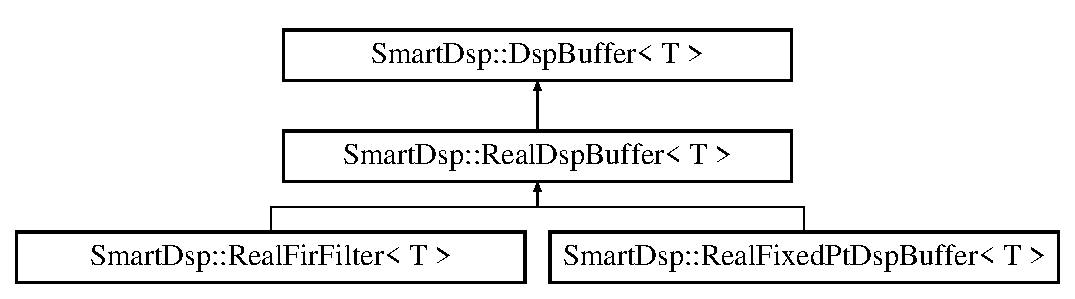
\includegraphics[height=3.000000cm]{class_smart_dsp_1_1_real_dsp_buffer}
\end{center}
\end{figure}
\subsection*{Public Member Functions}
\begin{DoxyCompactItemize}
\item 
\hyperlink{class_smart_dsp_1_1_real_dsp_buffer_ae5bd9282a607c876c85dfcf3d4c096c2}{Real\+Dsp\+Buffer} (void)
\item 
\hyperlink{class_smart_dsp_1_1_real_dsp_buffer_a0e3133404be83c2fb4272d89e719bfe6}{Real\+Dsp\+Buffer} (unsigned \hyperlink{class_smart_dsp_1_1_dsp_buffer_af931c57c26c1f459cae47ca4b249d402}{size})
\item 
{\footnotesize template$<$typename U $>$ }\\\hyperlink{class_smart_dsp_1_1_real_dsp_buffer_a49436d4de244c657abc1e85f7be3c9e0}{Real\+Dsp\+Buffer} (std\+::vector$<$ U $>$ data)
\item 
{\footnotesize template$<$typename U $>$ }\\\hyperlink{class_smart_dsp_1_1_real_dsp_buffer_a061791c79feca4c976512af36aa3e3b9}{Real\+Dsp\+Buffer} (U $\ast$data, unsigned data\+Len)
\item 
\hyperlink{class_smart_dsp_1_1_real_dsp_buffer_a8ee27b5155b47c1e0871c999d87f53be}{Real\+Dsp\+Buffer} (const \hyperlink{class_smart_dsp_1_1_real_dsp_buffer}{Real\+Dsp\+Buffer}$<$ T $>$ \&other)
\item 
\hyperlink{class_smart_dsp_1_1_real_dsp_buffer}{Real\+Dsp\+Buffer}$<$ T $>$ \& \hyperlink{class_smart_dsp_1_1_real_dsp_buffer_a59f770086f96d02c5ebbc2e8c2c32355}{operator=} (const \hyperlink{class_smart_dsp_1_1_dsp_buffer}{Dsp\+Buffer}$<$ T $>$ \&rhs)
\item 
\hyperlink{class_smart_dsp_1_1_real_dsp_buffer}{Real\+Dsp\+Buffer}$<$ T $>$ \& \hyperlink{class_smart_dsp_1_1_real_dsp_buffer_ab632957839103d9f2d86db3eaf1b8b5c}{pow} (const \hyperlink{_dsp_buffer_8h_a9ed4123d332590f7a6161bc2061eac49}{S\+M\+A\+R\+T\+D\+S\+P\+\_\+\+F\+L\+O\+A\+T\+\_\+\+T\+Y\+P\+E} exponent)
\item 
const \hyperlink{_dsp_buffer_8h_a9ed4123d332590f7a6161bc2061eac49}{S\+M\+A\+R\+T\+D\+S\+P\+\_\+\+F\+L\+O\+A\+T\+\_\+\+T\+Y\+P\+E} \hyperlink{class_smart_dsp_1_1_real_dsp_buffer_a731292861a4adf55385f14c3585274d6}{mean} () const 
\item 
const \hyperlink{_dsp_buffer_8h_a9ed4123d332590f7a6161bc2061eac49}{S\+M\+A\+R\+T\+D\+S\+P\+\_\+\+F\+L\+O\+A\+T\+\_\+\+T\+Y\+P\+E} \hyperlink{class_smart_dsp_1_1_real_dsp_buffer_a1d9b740ccc718fc524961091bd95367c}{var} () const 
\item 
const \hyperlink{_dsp_buffer_8h_a9ed4123d332590f7a6161bc2061eac49}{S\+M\+A\+R\+T\+D\+S\+P\+\_\+\+F\+L\+O\+A\+T\+\_\+\+T\+Y\+P\+E} \hyperlink{class_smart_dsp_1_1_real_dsp_buffer_a6a2ab5f40d6eec01389f2cc483c56889}{std\+Dev} () const 
\item 
const T \hyperlink{class_smart_dsp_1_1_real_dsp_buffer_ae4267e9c62b7edf852403e1ba9484dcb}{median} ()
\item 
const T \hyperlink{class_smart_dsp_1_1_real_dsp_buffer_ae2d2ffd71be7d6ad8606053d648ec965}{max} (unsigned $\ast$max\+Loc=N\+U\+L\+L) const 
\item 
const T \hyperlink{class_smart_dsp_1_1_real_dsp_buffer_a62eb35532a78dc8a8a99e050e61258f5}{min} (unsigned $\ast$min\+Loc=N\+U\+L\+L) const 
\item 
\hyperlink{class_smart_dsp_1_1_real_dsp_buffer}{Real\+Dsp\+Buffer}$<$ T $>$ \& \hyperlink{class_smart_dsp_1_1_real_dsp_buffer_a239ea8a1affb36ae6ce8ba6532902b19}{saturate} (T val)
\end{DoxyCompactItemize}
\subsection*{Additional Inherited Members}


\subsection{Detailed Description}
\subsubsection*{template$<$class T$>$class Smart\+Dsp\+::\+Real\+Dsp\+Buffer$<$ T $>$}



Definition at line 19 of file Real\+Dsp\+Buffer.\+h.



\subsection{Constructor \& Destructor Documentation}
\hypertarget{class_smart_dsp_1_1_real_dsp_buffer_ae5bd9282a607c876c85dfcf3d4c096c2}{\index{Smart\+Dsp\+::\+Real\+Dsp\+Buffer@{Smart\+Dsp\+::\+Real\+Dsp\+Buffer}!Real\+Dsp\+Buffer@{Real\+Dsp\+Buffer}}
\index{Real\+Dsp\+Buffer@{Real\+Dsp\+Buffer}!Smart\+Dsp\+::\+Real\+Dsp\+Buffer@{Smart\+Dsp\+::\+Real\+Dsp\+Buffer}}
\subsubsection[{Real\+Dsp\+Buffer}]{\setlength{\rightskip}{0pt plus 5cm}template$<$class T$>$ {\bf Smart\+Dsp\+::\+Real\+Dsp\+Buffer}$<$ T $>$\+::{\bf Real\+Dsp\+Buffer} (
\begin{DoxyParamCaption}
\item[{void}]{}
\end{DoxyParamCaption}
)\hspace{0.3cm}{\ttfamily [inline]}}}\label{class_smart_dsp_1_1_real_dsp_buffer_ae5bd9282a607c876c85dfcf3d4c096c2}


Definition at line 22 of file Real\+Dsp\+Buffer.\+h.

\hypertarget{class_smart_dsp_1_1_real_dsp_buffer_a0e3133404be83c2fb4272d89e719bfe6}{\index{Smart\+Dsp\+::\+Real\+Dsp\+Buffer@{Smart\+Dsp\+::\+Real\+Dsp\+Buffer}!Real\+Dsp\+Buffer@{Real\+Dsp\+Buffer}}
\index{Real\+Dsp\+Buffer@{Real\+Dsp\+Buffer}!Smart\+Dsp\+::\+Real\+Dsp\+Buffer@{Smart\+Dsp\+::\+Real\+Dsp\+Buffer}}
\subsubsection[{Real\+Dsp\+Buffer}]{\setlength{\rightskip}{0pt plus 5cm}template$<$class T$>$ {\bf Smart\+Dsp\+::\+Real\+Dsp\+Buffer}$<$ T $>$\+::{\bf Real\+Dsp\+Buffer} (
\begin{DoxyParamCaption}
\item[{unsigned}]{size}
\end{DoxyParamCaption}
)\hspace{0.3cm}{\ttfamily [inline]}}}\label{class_smart_dsp_1_1_real_dsp_buffer_a0e3133404be83c2fb4272d89e719bfe6}


Definition at line 23 of file Real\+Dsp\+Buffer.\+h.

\hypertarget{class_smart_dsp_1_1_real_dsp_buffer_a49436d4de244c657abc1e85f7be3c9e0}{\index{Smart\+Dsp\+::\+Real\+Dsp\+Buffer@{Smart\+Dsp\+::\+Real\+Dsp\+Buffer}!Real\+Dsp\+Buffer@{Real\+Dsp\+Buffer}}
\index{Real\+Dsp\+Buffer@{Real\+Dsp\+Buffer}!Smart\+Dsp\+::\+Real\+Dsp\+Buffer@{Smart\+Dsp\+::\+Real\+Dsp\+Buffer}}
\subsubsection[{Real\+Dsp\+Buffer}]{\setlength{\rightskip}{0pt plus 5cm}template$<$class T$>$ template$<$typename U $>$ {\bf Smart\+Dsp\+::\+Real\+Dsp\+Buffer}$<$ T $>$\+::{\bf Real\+Dsp\+Buffer} (
\begin{DoxyParamCaption}
\item[{std\+::vector$<$ U $>$}]{data}
\end{DoxyParamCaption}
)\hspace{0.3cm}{\ttfamily [inline]}}}\label{class_smart_dsp_1_1_real_dsp_buffer_a49436d4de244c657abc1e85f7be3c9e0}


Definition at line 25 of file Real\+Dsp\+Buffer.\+h.

\hypertarget{class_smart_dsp_1_1_real_dsp_buffer_a061791c79feca4c976512af36aa3e3b9}{\index{Smart\+Dsp\+::\+Real\+Dsp\+Buffer@{Smart\+Dsp\+::\+Real\+Dsp\+Buffer}!Real\+Dsp\+Buffer@{Real\+Dsp\+Buffer}}
\index{Real\+Dsp\+Buffer@{Real\+Dsp\+Buffer}!Smart\+Dsp\+::\+Real\+Dsp\+Buffer@{Smart\+Dsp\+::\+Real\+Dsp\+Buffer}}
\subsubsection[{Real\+Dsp\+Buffer}]{\setlength{\rightskip}{0pt plus 5cm}template$<$class T$>$ template$<$typename U $>$ {\bf Smart\+Dsp\+::\+Real\+Dsp\+Buffer}$<$ T $>$\+::{\bf Real\+Dsp\+Buffer} (
\begin{DoxyParamCaption}
\item[{U $\ast$}]{data, }
\item[{unsigned}]{data\+Len}
\end{DoxyParamCaption}
)\hspace{0.3cm}{\ttfamily [inline]}}}\label{class_smart_dsp_1_1_real_dsp_buffer_a061791c79feca4c976512af36aa3e3b9}


Definition at line 27 of file Real\+Dsp\+Buffer.\+h.

\hypertarget{class_smart_dsp_1_1_real_dsp_buffer_a8ee27b5155b47c1e0871c999d87f53be}{\index{Smart\+Dsp\+::\+Real\+Dsp\+Buffer@{Smart\+Dsp\+::\+Real\+Dsp\+Buffer}!Real\+Dsp\+Buffer@{Real\+Dsp\+Buffer}}
\index{Real\+Dsp\+Buffer@{Real\+Dsp\+Buffer}!Smart\+Dsp\+::\+Real\+Dsp\+Buffer@{Smart\+Dsp\+::\+Real\+Dsp\+Buffer}}
\subsubsection[{Real\+Dsp\+Buffer}]{\setlength{\rightskip}{0pt plus 5cm}template$<$class T$>$ {\bf Smart\+Dsp\+::\+Real\+Dsp\+Buffer}$<$ T $>$\+::{\bf Real\+Dsp\+Buffer} (
\begin{DoxyParamCaption}
\item[{const {\bf Real\+Dsp\+Buffer}$<$ T $>$ \&}]{other}
\end{DoxyParamCaption}
)\hspace{0.3cm}{\ttfamily [inline]}}}\label{class_smart_dsp_1_1_real_dsp_buffer_a8ee27b5155b47c1e0871c999d87f53be}


Definition at line 29 of file Real\+Dsp\+Buffer.\+h.



\subsection{Member Function Documentation}
\hypertarget{class_smart_dsp_1_1_real_dsp_buffer_ae2d2ffd71be7d6ad8606053d648ec965}{\index{Smart\+Dsp\+::\+Real\+Dsp\+Buffer@{Smart\+Dsp\+::\+Real\+Dsp\+Buffer}!max@{max}}
\index{max@{max}!Smart\+Dsp\+::\+Real\+Dsp\+Buffer@{Smart\+Dsp\+::\+Real\+Dsp\+Buffer}}
\subsubsection[{max}]{\setlength{\rightskip}{0pt plus 5cm}template$<$class T $>$ const T {\bf Smart\+Dsp\+::\+Real\+Dsp\+Buffer}$<$ T $>$\+::max (
\begin{DoxyParamCaption}
\item[{unsigned $\ast$}]{max\+Loc = {\ttfamily NULL}}
\end{DoxyParamCaption}
) const}}\label{class_smart_dsp_1_1_real_dsp_buffer_ae2d2ffd71be7d6ad8606053d648ec965}


Definition at line 117 of file Real\+Dsp\+Buffer.\+h.

\hypertarget{class_smart_dsp_1_1_real_dsp_buffer_a731292861a4adf55385f14c3585274d6}{\index{Smart\+Dsp\+::\+Real\+Dsp\+Buffer@{Smart\+Dsp\+::\+Real\+Dsp\+Buffer}!mean@{mean}}
\index{mean@{mean}!Smart\+Dsp\+::\+Real\+Dsp\+Buffer@{Smart\+Dsp\+::\+Real\+Dsp\+Buffer}}
\subsubsection[{mean}]{\setlength{\rightskip}{0pt plus 5cm}template$<$class T $>$ const {\bf S\+M\+A\+R\+T\+D\+S\+P\+\_\+\+F\+L\+O\+A\+T\+\_\+\+T\+Y\+P\+E} {\bf Smart\+Dsp\+::\+Real\+Dsp\+Buffer}$<$ T $>$\+::mean (
\begin{DoxyParamCaption}
{}
\end{DoxyParamCaption}
) const}}\label{class_smart_dsp_1_1_real_dsp_buffer_a731292861a4adf55385f14c3585274d6}


Definition at line 59 of file Real\+Dsp\+Buffer.\+h.

\hypertarget{class_smart_dsp_1_1_real_dsp_buffer_ae4267e9c62b7edf852403e1ba9484dcb}{\index{Smart\+Dsp\+::\+Real\+Dsp\+Buffer@{Smart\+Dsp\+::\+Real\+Dsp\+Buffer}!median@{median}}
\index{median@{median}!Smart\+Dsp\+::\+Real\+Dsp\+Buffer@{Smart\+Dsp\+::\+Real\+Dsp\+Buffer}}
\subsubsection[{median}]{\setlength{\rightskip}{0pt plus 5cm}template$<$class T $>$ const T {\bf Smart\+Dsp\+::\+Real\+Dsp\+Buffer}$<$ T $>$\+::median (
\begin{DoxyParamCaption}
{}
\end{DoxyParamCaption}
)}}\label{class_smart_dsp_1_1_real_dsp_buffer_ae4267e9c62b7edf852403e1ba9484dcb}


Definition at line 96 of file Real\+Dsp\+Buffer.\+h.

\hypertarget{class_smart_dsp_1_1_real_dsp_buffer_a62eb35532a78dc8a8a99e050e61258f5}{\index{Smart\+Dsp\+::\+Real\+Dsp\+Buffer@{Smart\+Dsp\+::\+Real\+Dsp\+Buffer}!min@{min}}
\index{min@{min}!Smart\+Dsp\+::\+Real\+Dsp\+Buffer@{Smart\+Dsp\+::\+Real\+Dsp\+Buffer}}
\subsubsection[{min}]{\setlength{\rightskip}{0pt plus 5cm}template$<$class T $>$ const T {\bf Smart\+Dsp\+::\+Real\+Dsp\+Buffer}$<$ T $>$\+::min (
\begin{DoxyParamCaption}
\item[{unsigned $\ast$}]{min\+Loc = {\ttfamily NULL}}
\end{DoxyParamCaption}
) const}}\label{class_smart_dsp_1_1_real_dsp_buffer_a62eb35532a78dc8a8a99e050e61258f5}


Definition at line 141 of file Real\+Dsp\+Buffer.\+h.

\hypertarget{class_smart_dsp_1_1_real_dsp_buffer_a59f770086f96d02c5ebbc2e8c2c32355}{\index{Smart\+Dsp\+::\+Real\+Dsp\+Buffer@{Smart\+Dsp\+::\+Real\+Dsp\+Buffer}!operator=@{operator=}}
\index{operator=@{operator=}!Smart\+Dsp\+::\+Real\+Dsp\+Buffer@{Smart\+Dsp\+::\+Real\+Dsp\+Buffer}}
\subsubsection[{operator=}]{\setlength{\rightskip}{0pt plus 5cm}template$<$class T$>$ {\bf Real\+Dsp\+Buffer}$<$T$>$\& {\bf Smart\+Dsp\+::\+Real\+Dsp\+Buffer}$<$ T $>$\+::operator= (
\begin{DoxyParamCaption}
\item[{const {\bf Dsp\+Buffer}$<$ T $>$ \&}]{rhs}
\end{DoxyParamCaption}
)\hspace{0.3cm}{\ttfamily [inline]}}}\label{class_smart_dsp_1_1_real_dsp_buffer_a59f770086f96d02c5ebbc2e8c2c32355}


Definition at line 30 of file Real\+Dsp\+Buffer.\+h.

\hypertarget{class_smart_dsp_1_1_real_dsp_buffer_ab632957839103d9f2d86db3eaf1b8b5c}{\index{Smart\+Dsp\+::\+Real\+Dsp\+Buffer@{Smart\+Dsp\+::\+Real\+Dsp\+Buffer}!pow@{pow}}
\index{pow@{pow}!Smart\+Dsp\+::\+Real\+Dsp\+Buffer@{Smart\+Dsp\+::\+Real\+Dsp\+Buffer}}
\subsubsection[{pow}]{\setlength{\rightskip}{0pt plus 5cm}template$<$class T $>$ {\bf Real\+Dsp\+Buffer}$<$ T $>$ \& {\bf Smart\+Dsp\+::\+Real\+Dsp\+Buffer}$<$ T $>$\+::pow (
\begin{DoxyParamCaption}
\item[{const {\bf S\+M\+A\+R\+T\+D\+S\+P\+\_\+\+F\+L\+O\+A\+T\+\_\+\+T\+Y\+P\+E}}]{exponent}
\end{DoxyParamCaption}
)}}\label{class_smart_dsp_1_1_real_dsp_buffer_ab632957839103d9f2d86db3eaf1b8b5c}


Definition at line 46 of file Real\+Dsp\+Buffer.\+h.

\hypertarget{class_smart_dsp_1_1_real_dsp_buffer_a239ea8a1affb36ae6ce8ba6532902b19}{\index{Smart\+Dsp\+::\+Real\+Dsp\+Buffer@{Smart\+Dsp\+::\+Real\+Dsp\+Buffer}!saturate@{saturate}}
\index{saturate@{saturate}!Smart\+Dsp\+::\+Real\+Dsp\+Buffer@{Smart\+Dsp\+::\+Real\+Dsp\+Buffer}}
\subsubsection[{saturate}]{\setlength{\rightskip}{0pt plus 5cm}template$<$class T $>$ {\bf Real\+Dsp\+Buffer}$<$ T $>$ \& {\bf Smart\+Dsp\+::\+Real\+Dsp\+Buffer}$<$ T $>$\+::saturate (
\begin{DoxyParamCaption}
\item[{T}]{val}
\end{DoxyParamCaption}
)}}\label{class_smart_dsp_1_1_real_dsp_buffer_a239ea8a1affb36ae6ce8ba6532902b19}


Definition at line 164 of file Real\+Dsp\+Buffer.\+h.

\hypertarget{class_smart_dsp_1_1_real_dsp_buffer_a6a2ab5f40d6eec01389f2cc483c56889}{\index{Smart\+Dsp\+::\+Real\+Dsp\+Buffer@{Smart\+Dsp\+::\+Real\+Dsp\+Buffer}!std\+Dev@{std\+Dev}}
\index{std\+Dev@{std\+Dev}!Smart\+Dsp\+::\+Real\+Dsp\+Buffer@{Smart\+Dsp\+::\+Real\+Dsp\+Buffer}}
\subsubsection[{std\+Dev}]{\setlength{\rightskip}{0pt plus 5cm}template$<$class T$>$ const {\bf S\+M\+A\+R\+T\+D\+S\+P\+\_\+\+F\+L\+O\+A\+T\+\_\+\+T\+Y\+P\+E} {\bf Smart\+Dsp\+::\+Real\+Dsp\+Buffer}$<$ T $>$\+::std\+Dev (
\begin{DoxyParamCaption}
{}
\end{DoxyParamCaption}
) const\hspace{0.3cm}{\ttfamily [inline]}}}\label{class_smart_dsp_1_1_real_dsp_buffer_a6a2ab5f40d6eec01389f2cc483c56889}


Definition at line 37 of file Real\+Dsp\+Buffer.\+h.

\hypertarget{class_smart_dsp_1_1_real_dsp_buffer_a1d9b740ccc718fc524961091bd95367c}{\index{Smart\+Dsp\+::\+Real\+Dsp\+Buffer@{Smart\+Dsp\+::\+Real\+Dsp\+Buffer}!var@{var}}
\index{var@{var}!Smart\+Dsp\+::\+Real\+Dsp\+Buffer@{Smart\+Dsp\+::\+Real\+Dsp\+Buffer}}
\subsubsection[{var}]{\setlength{\rightskip}{0pt plus 5cm}template$<$class T $>$ const {\bf S\+M\+A\+R\+T\+D\+S\+P\+\_\+\+F\+L\+O\+A\+T\+\_\+\+T\+Y\+P\+E} {\bf Smart\+Dsp\+::\+Real\+Dsp\+Buffer}$<$ T $>$\+::var (
\begin{DoxyParamCaption}
{}
\end{DoxyParamCaption}
) const}}\label{class_smart_dsp_1_1_real_dsp_buffer_a1d9b740ccc718fc524961091bd95367c}


Definition at line 74 of file Real\+Dsp\+Buffer.\+h.



The documentation for this class was generated from the following file\+:\begin{DoxyCompactItemize}
\item 
src/\hyperlink{_real_dsp_buffer_8h}{Real\+Dsp\+Buffer.\+h}\end{DoxyCompactItemize}

\hypertarget{class_smart_dsp_1_1_real_fir_filter}{\section{Smart\+Dsp\+:\+:Real\+Fir\+Filter$<$ T $>$ Class Template Reference}
\label{class_smart_dsp_1_1_real_fir_filter}\index{Smart\+Dsp\+::\+Real\+Fir\+Filter$<$ T $>$@{Smart\+Dsp\+::\+Real\+Fir\+Filter$<$ T $>$}}
}


{\ttfamily \#include $<$Real\+Fir\+Filter.\+h$>$}

Inheritance diagram for Smart\+Dsp\+:\+:Real\+Fir\+Filter$<$ T $>$\+:\begin{figure}[H]
\begin{center}
\leavevmode
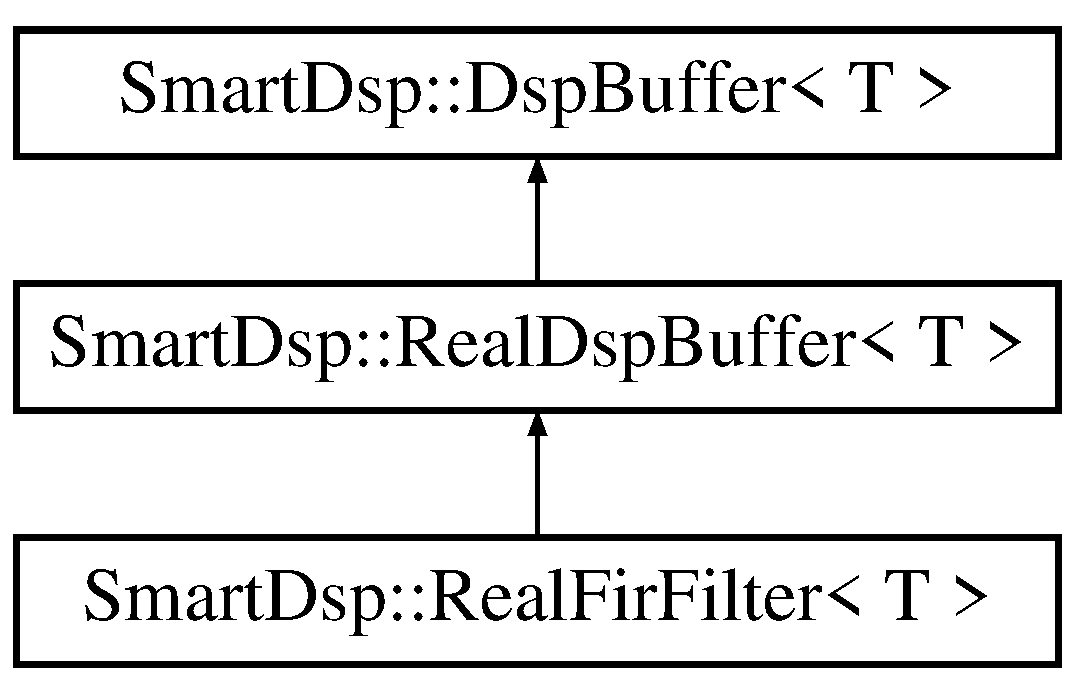
\includegraphics[height=3.000000cm]{class_smart_dsp_1_1_real_fir_filter}
\end{center}
\end{figure}
\subsection*{Public Member Functions}
\begin{DoxyCompactItemize}
\item 
\hyperlink{class_smart_dsp_1_1_real_fir_filter_afdef048d38c7f0c9ec3115f762066a72}{Real\+Fir\+Filter} (void)
\item 
\hyperlink{class_smart_dsp_1_1_real_fir_filter_a202a3515ae141bbf348bdc2c791c77ce}{Real\+Fir\+Filter} (unsigned \hyperlink{class_smart_dsp_1_1_dsp_buffer_af931c57c26c1f459cae47ca4b249d402}{size})
\item 
{\footnotesize template$<$typename U $>$ }\\\hyperlink{class_smart_dsp_1_1_real_fir_filter_a0be3bd0f15b082e2642dfe926844dc4c}{Real\+Fir\+Filter} (std\+::vector$<$ U $>$ data)
\item 
{\footnotesize template$<$typename U $>$ }\\\hyperlink{class_smart_dsp_1_1_real_fir_filter_af3f8b7baea3a554e92e4f2e851813e2b}{Real\+Fir\+Filter} (U $\ast$data, unsigned data\+Len)
\item 
\hyperlink{class_smart_dsp_1_1_real_fir_filter_a50fc0d776c2e76be49c389fe109baf84}{Real\+Fir\+Filter} (const \hyperlink{class_smart_dsp_1_1_real_fir_filter}{Real\+Fir\+Filter}$<$ T $>$ \&other)
\item 
\hyperlink{class_smart_dsp_1_1_real_fir_filter}{Real\+Fir\+Filter}$<$ T $>$ \& \hyperlink{class_smart_dsp_1_1_real_fir_filter_a79d51fc39a0fcd5ad8551e51976000b9}{operator=} (const \hyperlink{class_smart_dsp_1_1_dsp_buffer}{Dsp\+Buffer}$<$ T $>$ \&rhs)
\end{DoxyCompactItemize}
\subsection*{Protected Attributes}
\begin{DoxyCompactItemize}
\item 
std\+::vector$<$ T $>$ \hyperlink{class_smart_dsp_1_1_real_fir_filter_acdf8f2ace5e278eacb4517708de288a8}{state}
\end{DoxyCompactItemize}
\subsection*{Additional Inherited Members}


\subsection{Detailed Description}
\subsubsection*{template$<$class T$>$class Smart\+Dsp\+::\+Real\+Fir\+Filter$<$ T $>$}



Definition at line 20 of file Real\+Fir\+Filter.\+h.



\subsection{Constructor \& Destructor Documentation}
\hypertarget{class_smart_dsp_1_1_real_fir_filter_afdef048d38c7f0c9ec3115f762066a72}{\index{Smart\+Dsp\+::\+Real\+Fir\+Filter@{Smart\+Dsp\+::\+Real\+Fir\+Filter}!Real\+Fir\+Filter@{Real\+Fir\+Filter}}
\index{Real\+Fir\+Filter@{Real\+Fir\+Filter}!Smart\+Dsp\+::\+Real\+Fir\+Filter@{Smart\+Dsp\+::\+Real\+Fir\+Filter}}
\subsubsection[{Real\+Fir\+Filter}]{\setlength{\rightskip}{0pt plus 5cm}template$<$class T$>$ {\bf Smart\+Dsp\+::\+Real\+Fir\+Filter}$<$ T $>$\+::{\bf Real\+Fir\+Filter} (
\begin{DoxyParamCaption}
\item[{void}]{}
\end{DoxyParamCaption}
)\hspace{0.3cm}{\ttfamily [inline]}}}\label{class_smart_dsp_1_1_real_fir_filter_afdef048d38c7f0c9ec3115f762066a72}


Definition at line 26 of file Real\+Fir\+Filter.\+h.

\hypertarget{class_smart_dsp_1_1_real_fir_filter_a202a3515ae141bbf348bdc2c791c77ce}{\index{Smart\+Dsp\+::\+Real\+Fir\+Filter@{Smart\+Dsp\+::\+Real\+Fir\+Filter}!Real\+Fir\+Filter@{Real\+Fir\+Filter}}
\index{Real\+Fir\+Filter@{Real\+Fir\+Filter}!Smart\+Dsp\+::\+Real\+Fir\+Filter@{Smart\+Dsp\+::\+Real\+Fir\+Filter}}
\subsubsection[{Real\+Fir\+Filter}]{\setlength{\rightskip}{0pt plus 5cm}template$<$class T$>$ {\bf Smart\+Dsp\+::\+Real\+Fir\+Filter}$<$ T $>$\+::{\bf Real\+Fir\+Filter} (
\begin{DoxyParamCaption}
\item[{unsigned}]{size}
\end{DoxyParamCaption}
)\hspace{0.3cm}{\ttfamily [inline]}}}\label{class_smart_dsp_1_1_real_fir_filter_a202a3515ae141bbf348bdc2c791c77ce}


Definition at line 27 of file Real\+Fir\+Filter.\+h.

\hypertarget{class_smart_dsp_1_1_real_fir_filter_a0be3bd0f15b082e2642dfe926844dc4c}{\index{Smart\+Dsp\+::\+Real\+Fir\+Filter@{Smart\+Dsp\+::\+Real\+Fir\+Filter}!Real\+Fir\+Filter@{Real\+Fir\+Filter}}
\index{Real\+Fir\+Filter@{Real\+Fir\+Filter}!Smart\+Dsp\+::\+Real\+Fir\+Filter@{Smart\+Dsp\+::\+Real\+Fir\+Filter}}
\subsubsection[{Real\+Fir\+Filter}]{\setlength{\rightskip}{0pt plus 5cm}template$<$class T$>$ template$<$typename U $>$ {\bf Smart\+Dsp\+::\+Real\+Fir\+Filter}$<$ T $>$\+::{\bf Real\+Fir\+Filter} (
\begin{DoxyParamCaption}
\item[{std\+::vector$<$ U $>$}]{data}
\end{DoxyParamCaption}
)\hspace{0.3cm}{\ttfamily [inline]}}}\label{class_smart_dsp_1_1_real_fir_filter_a0be3bd0f15b082e2642dfe926844dc4c}


Definition at line 29 of file Real\+Fir\+Filter.\+h.

\hypertarget{class_smart_dsp_1_1_real_fir_filter_af3f8b7baea3a554e92e4f2e851813e2b}{\index{Smart\+Dsp\+::\+Real\+Fir\+Filter@{Smart\+Dsp\+::\+Real\+Fir\+Filter}!Real\+Fir\+Filter@{Real\+Fir\+Filter}}
\index{Real\+Fir\+Filter@{Real\+Fir\+Filter}!Smart\+Dsp\+::\+Real\+Fir\+Filter@{Smart\+Dsp\+::\+Real\+Fir\+Filter}}
\subsubsection[{Real\+Fir\+Filter}]{\setlength{\rightskip}{0pt plus 5cm}template$<$class T$>$ template$<$typename U $>$ {\bf Smart\+Dsp\+::\+Real\+Fir\+Filter}$<$ T $>$\+::{\bf Real\+Fir\+Filter} (
\begin{DoxyParamCaption}
\item[{U $\ast$}]{data, }
\item[{unsigned}]{data\+Len}
\end{DoxyParamCaption}
)\hspace{0.3cm}{\ttfamily [inline]}}}\label{class_smart_dsp_1_1_real_fir_filter_af3f8b7baea3a554e92e4f2e851813e2b}


Definition at line 31 of file Real\+Fir\+Filter.\+h.

\hypertarget{class_smart_dsp_1_1_real_fir_filter_a50fc0d776c2e76be49c389fe109baf84}{\index{Smart\+Dsp\+::\+Real\+Fir\+Filter@{Smart\+Dsp\+::\+Real\+Fir\+Filter}!Real\+Fir\+Filter@{Real\+Fir\+Filter}}
\index{Real\+Fir\+Filter@{Real\+Fir\+Filter}!Smart\+Dsp\+::\+Real\+Fir\+Filter@{Smart\+Dsp\+::\+Real\+Fir\+Filter}}
\subsubsection[{Real\+Fir\+Filter}]{\setlength{\rightskip}{0pt plus 5cm}template$<$class T$>$ {\bf Smart\+Dsp\+::\+Real\+Fir\+Filter}$<$ T $>$\+::{\bf Real\+Fir\+Filter} (
\begin{DoxyParamCaption}
\item[{const {\bf Real\+Fir\+Filter}$<$ T $>$ \&}]{other}
\end{DoxyParamCaption}
)\hspace{0.3cm}{\ttfamily [inline]}}}\label{class_smart_dsp_1_1_real_fir_filter_a50fc0d776c2e76be49c389fe109baf84}


Definition at line 33 of file Real\+Fir\+Filter.\+h.



\subsection{Member Function Documentation}
\hypertarget{class_smart_dsp_1_1_real_fir_filter_a79d51fc39a0fcd5ad8551e51976000b9}{\index{Smart\+Dsp\+::\+Real\+Fir\+Filter@{Smart\+Dsp\+::\+Real\+Fir\+Filter}!operator=@{operator=}}
\index{operator=@{operator=}!Smart\+Dsp\+::\+Real\+Fir\+Filter@{Smart\+Dsp\+::\+Real\+Fir\+Filter}}
\subsubsection[{operator=}]{\setlength{\rightskip}{0pt plus 5cm}template$<$class T $>$ {\bf Real\+Fir\+Filter}$<$ T $>$ \& {\bf Smart\+Dsp\+::\+Real\+Fir\+Filter}$<$ T $>$\+::operator= (
\begin{DoxyParamCaption}
\item[{const {\bf Dsp\+Buffer}$<$ T $>$ \&}]{rhs}
\end{DoxyParamCaption}
)}}\label{class_smart_dsp_1_1_real_fir_filter_a79d51fc39a0fcd5ad8551e51976000b9}


Definition at line 41 of file Real\+Fir\+Filter.\+h.



\subsection{Member Data Documentation}
\hypertarget{class_smart_dsp_1_1_real_fir_filter_acdf8f2ace5e278eacb4517708de288a8}{\index{Smart\+Dsp\+::\+Real\+Fir\+Filter@{Smart\+Dsp\+::\+Real\+Fir\+Filter}!state@{state}}
\index{state@{state}!Smart\+Dsp\+::\+Real\+Fir\+Filter@{Smart\+Dsp\+::\+Real\+Fir\+Filter}}
\subsubsection[{state}]{\setlength{\rightskip}{0pt plus 5cm}template$<$class T$>$ std\+::vector$<$T$>$ {\bf Smart\+Dsp\+::\+Real\+Fir\+Filter}$<$ T $>$\+::state\hspace{0.3cm}{\ttfamily [protected]}}}\label{class_smart_dsp_1_1_real_fir_filter_acdf8f2ace5e278eacb4517708de288a8}


Definition at line 22 of file Real\+Fir\+Filter.\+h.



The documentation for this class was generated from the following file\+:\begin{DoxyCompactItemize}
\item 
src/\hyperlink{_real_fir_filter_8h}{Real\+Fir\+Filter.\+h}\end{DoxyCompactItemize}

\hypertarget{class_smart_dsp_1_1_real_fixed_pt_dsp_buffer}{\section{Smart\+Dsp\+:\+:Real\+Fixed\+Pt\+Dsp\+Buffer$<$ T $>$ Class Template Reference}
\label{class_smart_dsp_1_1_real_fixed_pt_dsp_buffer}\index{Smart\+Dsp\+::\+Real\+Fixed\+Pt\+Dsp\+Buffer$<$ T $>$@{Smart\+Dsp\+::\+Real\+Fixed\+Pt\+Dsp\+Buffer$<$ T $>$}}
}


{\ttfamily \#include $<$Real\+Fixed\+Pt\+Dsp\+Buffer.\+h$>$}

Inheritance diagram for Smart\+Dsp\+:\+:Real\+Fixed\+Pt\+Dsp\+Buffer$<$ T $>$\+:\begin{figure}[H]
\begin{center}
\leavevmode
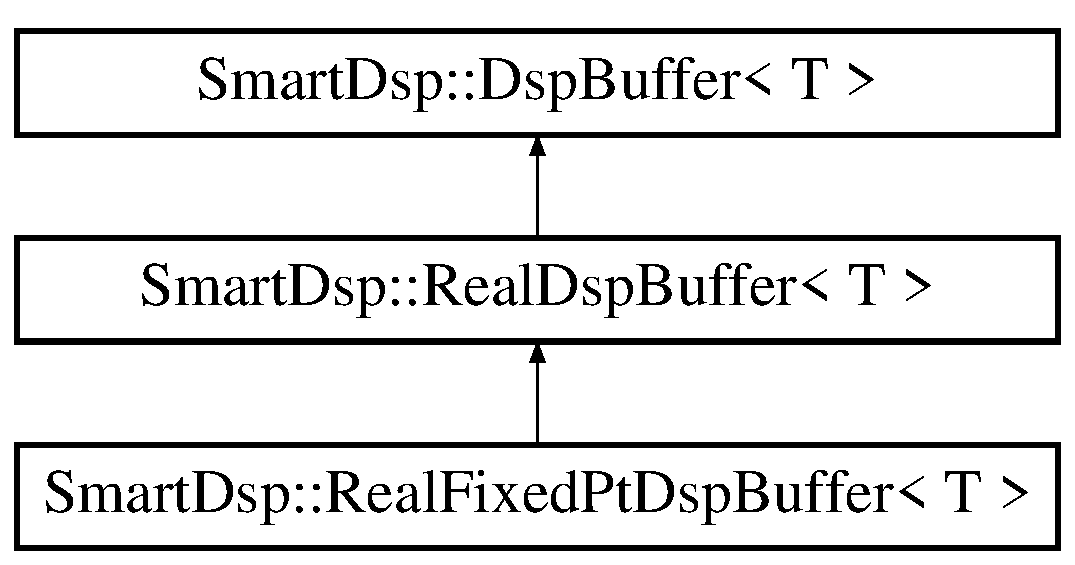
\includegraphics[height=3.000000cm]{class_smart_dsp_1_1_real_fixed_pt_dsp_buffer}
\end{center}
\end{figure}
\subsection*{Public Member Functions}
\begin{DoxyCompactItemize}
\item 
\hyperlink{class_smart_dsp_1_1_real_fixed_pt_dsp_buffer_ae3c3dff095c4fccdf05e91232c83ee9e}{Real\+Fixed\+Pt\+Dsp\+Buffer} (void)
\item 
\hyperlink{class_smart_dsp_1_1_real_fixed_pt_dsp_buffer_a3675f6676a342a7ca860fc8dc7ecc789}{Real\+Fixed\+Pt\+Dsp\+Buffer} (unsigned \hyperlink{class_smart_dsp_1_1_dsp_buffer_af931c57c26c1f459cae47ca4b249d402}{size})
\item 
{\footnotesize template$<$typename U $>$ }\\\hyperlink{class_smart_dsp_1_1_real_fixed_pt_dsp_buffer_a1338271bd75f8f668d703dece1957931}{Real\+Fixed\+Pt\+Dsp\+Buffer} (std\+::vector$<$ U $>$ data)
\item 
{\footnotesize template$<$typename U $>$ }\\\hyperlink{class_smart_dsp_1_1_real_fixed_pt_dsp_buffer_a3a0028bd8744466850067d580c6bbf18}{Real\+Fixed\+Pt\+Dsp\+Buffer} (U $\ast$data, unsigned data\+Len)
\item 
\hyperlink{class_smart_dsp_1_1_real_fixed_pt_dsp_buffer_ae07175e7317ee6451e9614d414832399}{Real\+Fixed\+Pt\+Dsp\+Buffer} (const \hyperlink{class_smart_dsp_1_1_real_fixed_pt_dsp_buffer}{Real\+Fixed\+Pt\+Dsp\+Buffer}$<$ T $>$ \&other)
\item 
\hyperlink{class_smart_dsp_1_1_real_fixed_pt_dsp_buffer}{Real\+Fixed\+Pt\+Dsp\+Buffer}$<$ T $>$ \& \hyperlink{class_smart_dsp_1_1_real_fixed_pt_dsp_buffer_a64978f7aadb02d9832cda903e2540341}{operator=} (const \hyperlink{class_smart_dsp_1_1_dsp_buffer}{Dsp\+Buffer}$<$ T $>$ \&rhs)
\item 
\hyperlink{class_smart_dsp_1_1_real_fixed_pt_dsp_buffer}{Real\+Fixed\+Pt\+Dsp\+Buffer}$<$ T $>$ \& \hyperlink{class_smart_dsp_1_1_real_fixed_pt_dsp_buffer_a27dc913f1d7059fbc2b574a0ee5d6d65}{operator++} ()
\item 
\hyperlink{class_smart_dsp_1_1_real_fixed_pt_dsp_buffer}{Real\+Fixed\+Pt\+Dsp\+Buffer}$<$ T $>$ \hyperlink{class_smart_dsp_1_1_real_fixed_pt_dsp_buffer_a8add599d8a19aa8641679485046cf1d2}{operator++} (int)
\item 
\hyperlink{class_smart_dsp_1_1_real_fixed_pt_dsp_buffer}{Real\+Fixed\+Pt\+Dsp\+Buffer}$<$ T $>$ \& \hyperlink{class_smart_dsp_1_1_real_fixed_pt_dsp_buffer_a9c06942aa4976915810cf8e026b3a02a}{operator-\/-\/} ()
\item 
\hyperlink{class_smart_dsp_1_1_real_fixed_pt_dsp_buffer}{Real\+Fixed\+Pt\+Dsp\+Buffer}$<$ T $>$ \hyperlink{class_smart_dsp_1_1_real_fixed_pt_dsp_buffer_a35ad28b40e01e70a2b3df7632db29dbe}{operator-\/-\/} (int)
\item 
{\footnotesize template$<$class U $>$ }\\\hyperlink{class_smart_dsp_1_1_real_fixed_pt_dsp_buffer}{Real\+Fixed\+Pt\+Dsp\+Buffer}$<$ T $>$ \& \hyperlink{class_smart_dsp_1_1_real_fixed_pt_dsp_buffer_a5975e80a29a4e2cc4fb9e40f888e2ba5}{operator\%=} (const \hyperlink{class_smart_dsp_1_1_real_fixed_pt_dsp_buffer}{Real\+Fixed\+Pt\+Dsp\+Buffer}$<$ U $>$ \&rhs)
\item 
\hyperlink{class_smart_dsp_1_1_real_fixed_pt_dsp_buffer}{Real\+Fixed\+Pt\+Dsp\+Buffer}$<$ T $>$ \& \hyperlink{class_smart_dsp_1_1_real_fixed_pt_dsp_buffer_a75b899c29ce4f717088e0ead1f381356}{operator\%=} (const T \&rhs)
\item 
\hyperlink{class_smart_dsp_1_1_real_fixed_pt_dsp_buffer}{Real\+Fixed\+Pt\+Dsp\+Buffer}$<$ T $>$ \& \hyperlink{class_smart_dsp_1_1_real_fixed_pt_dsp_buffer_aedaa0814160c15898bd95d27aa5b39d3}{operator$\sim$} ()
\item 
{\footnotesize template$<$class U $>$ }\\\hyperlink{class_smart_dsp_1_1_real_fixed_pt_dsp_buffer}{Real\+Fixed\+Pt\+Dsp\+Buffer}$<$ T $>$ \& \hyperlink{class_smart_dsp_1_1_real_fixed_pt_dsp_buffer_a65c8caae202586ced532eda353a3769c}{operator\&=} (const \hyperlink{class_smart_dsp_1_1_real_fixed_pt_dsp_buffer}{Real\+Fixed\+Pt\+Dsp\+Buffer}$<$ U $>$ \&rhs)
\item 
\hyperlink{class_smart_dsp_1_1_real_fixed_pt_dsp_buffer}{Real\+Fixed\+Pt\+Dsp\+Buffer}$<$ T $>$ \& \hyperlink{class_smart_dsp_1_1_real_fixed_pt_dsp_buffer_a44205d17e56c6aab520b6c3ede332f86}{operator\&=} (const T \&rhs)
\item 
{\footnotesize template$<$class U $>$ }\\\hyperlink{class_smart_dsp_1_1_real_fixed_pt_dsp_buffer}{Real\+Fixed\+Pt\+Dsp\+Buffer}$<$ T $>$ \& \hyperlink{class_smart_dsp_1_1_real_fixed_pt_dsp_buffer_abb91aac2de8fb64f2212f8b1f4d10749}{operator$\vert$=} (const \hyperlink{class_smart_dsp_1_1_real_fixed_pt_dsp_buffer}{Real\+Fixed\+Pt\+Dsp\+Buffer}$<$ U $>$ \&rhs)
\item 
\hyperlink{class_smart_dsp_1_1_real_fixed_pt_dsp_buffer}{Real\+Fixed\+Pt\+Dsp\+Buffer}$<$ T $>$ \& \hyperlink{class_smart_dsp_1_1_real_fixed_pt_dsp_buffer_a433746a971e30e5e622057ea6460b704}{operator$\vert$=} (const T \&rhs)
\item 
{\footnotesize template$<$class U $>$ }\\\hyperlink{class_smart_dsp_1_1_real_fixed_pt_dsp_buffer}{Real\+Fixed\+Pt\+Dsp\+Buffer}$<$ T $>$ \& \hyperlink{class_smart_dsp_1_1_real_fixed_pt_dsp_buffer_a4c40baa57ae2f4cfc919eaca5c4cb999}{operator$^\wedge$=} (const \hyperlink{class_smart_dsp_1_1_real_fixed_pt_dsp_buffer}{Real\+Fixed\+Pt\+Dsp\+Buffer}$<$ U $>$ \&rhs)
\item 
\hyperlink{class_smart_dsp_1_1_real_fixed_pt_dsp_buffer}{Real\+Fixed\+Pt\+Dsp\+Buffer}$<$ T $>$ \& \hyperlink{class_smart_dsp_1_1_real_fixed_pt_dsp_buffer_af20c35cfbc0d69a5e24766ecd4984022}{operator$^\wedge$=} (const T \&rhs)
\item 
{\footnotesize template$<$class U $>$ }\\\hyperlink{class_smart_dsp_1_1_real_fixed_pt_dsp_buffer}{Real\+Fixed\+Pt\+Dsp\+Buffer}$<$ T $>$ \& \hyperlink{class_smart_dsp_1_1_real_fixed_pt_dsp_buffer_a7f6d2c641c4e827fe9f02ba11bb2d3c3}{operator$>$$>$=} (const \hyperlink{class_smart_dsp_1_1_real_fixed_pt_dsp_buffer}{Real\+Fixed\+Pt\+Dsp\+Buffer}$<$ U $>$ \&rhs)
\item 
\hyperlink{class_smart_dsp_1_1_real_fixed_pt_dsp_buffer}{Real\+Fixed\+Pt\+Dsp\+Buffer}$<$ T $>$ \& \hyperlink{class_smart_dsp_1_1_real_fixed_pt_dsp_buffer_a733c7adf5561680dddf02acc8ad857ed}{operator$>$$>$=} (const T \&rhs)
\item 
{\footnotesize template$<$class U $>$ }\\\hyperlink{class_smart_dsp_1_1_real_fixed_pt_dsp_buffer}{Real\+Fixed\+Pt\+Dsp\+Buffer}$<$ T $>$ \& \hyperlink{class_smart_dsp_1_1_real_fixed_pt_dsp_buffer_a3a2420192b47c2f4e104410247445841}{operator$<$$<$=} (const \hyperlink{class_smart_dsp_1_1_real_fixed_pt_dsp_buffer}{Real\+Fixed\+Pt\+Dsp\+Buffer}$<$ U $>$ \&rhs)
\item 
\hyperlink{class_smart_dsp_1_1_real_fixed_pt_dsp_buffer}{Real\+Fixed\+Pt\+Dsp\+Buffer}$<$ T $>$ \& \hyperlink{class_smart_dsp_1_1_real_fixed_pt_dsp_buffer_a6c4ce36df966d4b3df40cbf4264fcba0}{operator$<$$<$=} (const T \&rhs)
\item 
\hyperlink{class_smart_dsp_1_1_real_dsp_buffer}{Real\+Dsp\+Buffer}$<$ T $>$ \& \hyperlink{class_smart_dsp_1_1_real_fixed_pt_dsp_buffer_a18baa3dd00f8f78b46c22086859ddd53}{pow} (const \hyperlink{_dsp_buffer_8h_a9ed4123d332590f7a6161bc2061eac49}{S\+M\+A\+R\+T\+D\+S\+P\+\_\+\+F\+L\+O\+A\+T\+\_\+\+T\+Y\+P\+E} exponent)
\item 
const T \hyperlink{class_smart_dsp_1_1_real_fixed_pt_dsp_buffer_a808320927290a8bbb67a14197cf46f9f}{mode} ()
\end{DoxyCompactItemize}
\subsection*{Additional Inherited Members}


\subsection{Detailed Description}
\subsubsection*{template$<$class T$>$class Smart\+Dsp\+::\+Real\+Fixed\+Pt\+Dsp\+Buffer$<$ T $>$}



Definition at line 20 of file Real\+Fixed\+Pt\+Dsp\+Buffer.\+h.



\subsection{Constructor \& Destructor Documentation}
\hypertarget{class_smart_dsp_1_1_real_fixed_pt_dsp_buffer_ae3c3dff095c4fccdf05e91232c83ee9e}{\index{Smart\+Dsp\+::\+Real\+Fixed\+Pt\+Dsp\+Buffer@{Smart\+Dsp\+::\+Real\+Fixed\+Pt\+Dsp\+Buffer}!Real\+Fixed\+Pt\+Dsp\+Buffer@{Real\+Fixed\+Pt\+Dsp\+Buffer}}
\index{Real\+Fixed\+Pt\+Dsp\+Buffer@{Real\+Fixed\+Pt\+Dsp\+Buffer}!Smart\+Dsp\+::\+Real\+Fixed\+Pt\+Dsp\+Buffer@{Smart\+Dsp\+::\+Real\+Fixed\+Pt\+Dsp\+Buffer}}
\subsubsection[{Real\+Fixed\+Pt\+Dsp\+Buffer}]{\setlength{\rightskip}{0pt plus 5cm}template$<$class T$>$ {\bf Smart\+Dsp\+::\+Real\+Fixed\+Pt\+Dsp\+Buffer}$<$ T $>$\+::{\bf Real\+Fixed\+Pt\+Dsp\+Buffer} (
\begin{DoxyParamCaption}
\item[{void}]{}
\end{DoxyParamCaption}
)\hspace{0.3cm}{\ttfamily [inline]}}}\label{class_smart_dsp_1_1_real_fixed_pt_dsp_buffer_ae3c3dff095c4fccdf05e91232c83ee9e}


Definition at line 23 of file Real\+Fixed\+Pt\+Dsp\+Buffer.\+h.

\hypertarget{class_smart_dsp_1_1_real_fixed_pt_dsp_buffer_a3675f6676a342a7ca860fc8dc7ecc789}{\index{Smart\+Dsp\+::\+Real\+Fixed\+Pt\+Dsp\+Buffer@{Smart\+Dsp\+::\+Real\+Fixed\+Pt\+Dsp\+Buffer}!Real\+Fixed\+Pt\+Dsp\+Buffer@{Real\+Fixed\+Pt\+Dsp\+Buffer}}
\index{Real\+Fixed\+Pt\+Dsp\+Buffer@{Real\+Fixed\+Pt\+Dsp\+Buffer}!Smart\+Dsp\+::\+Real\+Fixed\+Pt\+Dsp\+Buffer@{Smart\+Dsp\+::\+Real\+Fixed\+Pt\+Dsp\+Buffer}}
\subsubsection[{Real\+Fixed\+Pt\+Dsp\+Buffer}]{\setlength{\rightskip}{0pt plus 5cm}template$<$class T$>$ {\bf Smart\+Dsp\+::\+Real\+Fixed\+Pt\+Dsp\+Buffer}$<$ T $>$\+::{\bf Real\+Fixed\+Pt\+Dsp\+Buffer} (
\begin{DoxyParamCaption}
\item[{unsigned}]{size}
\end{DoxyParamCaption}
)\hspace{0.3cm}{\ttfamily [inline]}}}\label{class_smart_dsp_1_1_real_fixed_pt_dsp_buffer_a3675f6676a342a7ca860fc8dc7ecc789}


Definition at line 24 of file Real\+Fixed\+Pt\+Dsp\+Buffer.\+h.

\hypertarget{class_smart_dsp_1_1_real_fixed_pt_dsp_buffer_a1338271bd75f8f668d703dece1957931}{\index{Smart\+Dsp\+::\+Real\+Fixed\+Pt\+Dsp\+Buffer@{Smart\+Dsp\+::\+Real\+Fixed\+Pt\+Dsp\+Buffer}!Real\+Fixed\+Pt\+Dsp\+Buffer@{Real\+Fixed\+Pt\+Dsp\+Buffer}}
\index{Real\+Fixed\+Pt\+Dsp\+Buffer@{Real\+Fixed\+Pt\+Dsp\+Buffer}!Smart\+Dsp\+::\+Real\+Fixed\+Pt\+Dsp\+Buffer@{Smart\+Dsp\+::\+Real\+Fixed\+Pt\+Dsp\+Buffer}}
\subsubsection[{Real\+Fixed\+Pt\+Dsp\+Buffer}]{\setlength{\rightskip}{0pt plus 5cm}template$<$class T$>$ template$<$typename U $>$ {\bf Smart\+Dsp\+::\+Real\+Fixed\+Pt\+Dsp\+Buffer}$<$ T $>$\+::{\bf Real\+Fixed\+Pt\+Dsp\+Buffer} (
\begin{DoxyParamCaption}
\item[{std\+::vector$<$ U $>$}]{data}
\end{DoxyParamCaption}
)\hspace{0.3cm}{\ttfamily [inline]}}}\label{class_smart_dsp_1_1_real_fixed_pt_dsp_buffer_a1338271bd75f8f668d703dece1957931}


Definition at line 26 of file Real\+Fixed\+Pt\+Dsp\+Buffer.\+h.

\hypertarget{class_smart_dsp_1_1_real_fixed_pt_dsp_buffer_a3a0028bd8744466850067d580c6bbf18}{\index{Smart\+Dsp\+::\+Real\+Fixed\+Pt\+Dsp\+Buffer@{Smart\+Dsp\+::\+Real\+Fixed\+Pt\+Dsp\+Buffer}!Real\+Fixed\+Pt\+Dsp\+Buffer@{Real\+Fixed\+Pt\+Dsp\+Buffer}}
\index{Real\+Fixed\+Pt\+Dsp\+Buffer@{Real\+Fixed\+Pt\+Dsp\+Buffer}!Smart\+Dsp\+::\+Real\+Fixed\+Pt\+Dsp\+Buffer@{Smart\+Dsp\+::\+Real\+Fixed\+Pt\+Dsp\+Buffer}}
\subsubsection[{Real\+Fixed\+Pt\+Dsp\+Buffer}]{\setlength{\rightskip}{0pt plus 5cm}template$<$class T$>$ template$<$typename U $>$ {\bf Smart\+Dsp\+::\+Real\+Fixed\+Pt\+Dsp\+Buffer}$<$ T $>$\+::{\bf Real\+Fixed\+Pt\+Dsp\+Buffer} (
\begin{DoxyParamCaption}
\item[{U $\ast$}]{data, }
\item[{unsigned}]{data\+Len}
\end{DoxyParamCaption}
)\hspace{0.3cm}{\ttfamily [inline]}}}\label{class_smart_dsp_1_1_real_fixed_pt_dsp_buffer_a3a0028bd8744466850067d580c6bbf18}


Definition at line 28 of file Real\+Fixed\+Pt\+Dsp\+Buffer.\+h.

\hypertarget{class_smart_dsp_1_1_real_fixed_pt_dsp_buffer_ae07175e7317ee6451e9614d414832399}{\index{Smart\+Dsp\+::\+Real\+Fixed\+Pt\+Dsp\+Buffer@{Smart\+Dsp\+::\+Real\+Fixed\+Pt\+Dsp\+Buffer}!Real\+Fixed\+Pt\+Dsp\+Buffer@{Real\+Fixed\+Pt\+Dsp\+Buffer}}
\index{Real\+Fixed\+Pt\+Dsp\+Buffer@{Real\+Fixed\+Pt\+Dsp\+Buffer}!Smart\+Dsp\+::\+Real\+Fixed\+Pt\+Dsp\+Buffer@{Smart\+Dsp\+::\+Real\+Fixed\+Pt\+Dsp\+Buffer}}
\subsubsection[{Real\+Fixed\+Pt\+Dsp\+Buffer}]{\setlength{\rightskip}{0pt plus 5cm}template$<$class T$>$ {\bf Smart\+Dsp\+::\+Real\+Fixed\+Pt\+Dsp\+Buffer}$<$ T $>$\+::{\bf Real\+Fixed\+Pt\+Dsp\+Buffer} (
\begin{DoxyParamCaption}
\item[{const {\bf Real\+Fixed\+Pt\+Dsp\+Buffer}$<$ T $>$ \&}]{other}
\end{DoxyParamCaption}
)\hspace{0.3cm}{\ttfamily [inline]}}}\label{class_smart_dsp_1_1_real_fixed_pt_dsp_buffer_ae07175e7317ee6451e9614d414832399}


Definition at line 30 of file Real\+Fixed\+Pt\+Dsp\+Buffer.\+h.



\subsection{Member Function Documentation}
\hypertarget{class_smart_dsp_1_1_real_fixed_pt_dsp_buffer_a808320927290a8bbb67a14197cf46f9f}{\index{Smart\+Dsp\+::\+Real\+Fixed\+Pt\+Dsp\+Buffer@{Smart\+Dsp\+::\+Real\+Fixed\+Pt\+Dsp\+Buffer}!mode@{mode}}
\index{mode@{mode}!Smart\+Dsp\+::\+Real\+Fixed\+Pt\+Dsp\+Buffer@{Smart\+Dsp\+::\+Real\+Fixed\+Pt\+Dsp\+Buffer}}
\subsubsection[{mode}]{\setlength{\rightskip}{0pt plus 5cm}template$<$class T $>$ const T {\bf Smart\+Dsp\+::\+Real\+Fixed\+Pt\+Dsp\+Buffer}$<$ T $>$\+::mode (
\begin{DoxyParamCaption}
{}
\end{DoxyParamCaption}
)}}\label{class_smart_dsp_1_1_real_fixed_pt_dsp_buffer_a808320927290a8bbb67a14197cf46f9f}


Definition at line 329 of file Real\+Fixed\+Pt\+Dsp\+Buffer.\+h.

\hypertarget{class_smart_dsp_1_1_real_fixed_pt_dsp_buffer_a5975e80a29a4e2cc4fb9e40f888e2ba5}{\index{Smart\+Dsp\+::\+Real\+Fixed\+Pt\+Dsp\+Buffer@{Smart\+Dsp\+::\+Real\+Fixed\+Pt\+Dsp\+Buffer}!operator\%=@{operator\%=}}
\index{operator\%=@{operator\%=}!Smart\+Dsp\+::\+Real\+Fixed\+Pt\+Dsp\+Buffer@{Smart\+Dsp\+::\+Real\+Fixed\+Pt\+Dsp\+Buffer}}
\subsubsection[{operator\%=}]{\setlength{\rightskip}{0pt plus 5cm}template$<$class T $>$ template$<$class U $>$ {\bf Real\+Fixed\+Pt\+Dsp\+Buffer}$<$ T $>$ \& {\bf Smart\+Dsp\+::\+Real\+Fixed\+Pt\+Dsp\+Buffer}$<$ T $>$\+::operator\%= (
\begin{DoxyParamCaption}
\item[{const {\bf Real\+Fixed\+Pt\+Dsp\+Buffer}$<$ U $>$ \&}]{rhs}
\end{DoxyParamCaption}
)}}\label{class_smart_dsp_1_1_real_fixed_pt_dsp_buffer_a5975e80a29a4e2cc4fb9e40f888e2ba5}


Definition at line 109 of file Real\+Fixed\+Pt\+Dsp\+Buffer.\+h.

\hypertarget{class_smart_dsp_1_1_real_fixed_pt_dsp_buffer_a75b899c29ce4f717088e0ead1f381356}{\index{Smart\+Dsp\+::\+Real\+Fixed\+Pt\+Dsp\+Buffer@{Smart\+Dsp\+::\+Real\+Fixed\+Pt\+Dsp\+Buffer}!operator\%=@{operator\%=}}
\index{operator\%=@{operator\%=}!Smart\+Dsp\+::\+Real\+Fixed\+Pt\+Dsp\+Buffer@{Smart\+Dsp\+::\+Real\+Fixed\+Pt\+Dsp\+Buffer}}
\subsubsection[{operator\%=}]{\setlength{\rightskip}{0pt plus 5cm}template$<$class T $>$ {\bf Real\+Fixed\+Pt\+Dsp\+Buffer}$<$ T $>$ \& {\bf Smart\+Dsp\+::\+Real\+Fixed\+Pt\+Dsp\+Buffer}$<$ T $>$\+::operator\%= (
\begin{DoxyParamCaption}
\item[{const T \&}]{rhs}
\end{DoxyParamCaption}
)}}\label{class_smart_dsp_1_1_real_fixed_pt_dsp_buffer_a75b899c29ce4f717088e0ead1f381356}


Definition at line 119 of file Real\+Fixed\+Pt\+Dsp\+Buffer.\+h.

\hypertarget{class_smart_dsp_1_1_real_fixed_pt_dsp_buffer_a65c8caae202586ced532eda353a3769c}{\index{Smart\+Dsp\+::\+Real\+Fixed\+Pt\+Dsp\+Buffer@{Smart\+Dsp\+::\+Real\+Fixed\+Pt\+Dsp\+Buffer}!operator\&=@{operator\&=}}
\index{operator\&=@{operator\&=}!Smart\+Dsp\+::\+Real\+Fixed\+Pt\+Dsp\+Buffer@{Smart\+Dsp\+::\+Real\+Fixed\+Pt\+Dsp\+Buffer}}
\subsubsection[{operator\&=}]{\setlength{\rightskip}{0pt plus 5cm}template$<$class T $>$ template$<$class U $>$ {\bf Real\+Fixed\+Pt\+Dsp\+Buffer}$<$ T $>$ \& {\bf Smart\+Dsp\+::\+Real\+Fixed\+Pt\+Dsp\+Buffer}$<$ T $>$\+::operator\&= (
\begin{DoxyParamCaption}
\item[{const {\bf Real\+Fixed\+Pt\+Dsp\+Buffer}$<$ U $>$ \&}]{rhs}
\end{DoxyParamCaption}
)}}\label{class_smart_dsp_1_1_real_fixed_pt_dsp_buffer_a65c8caae202586ced532eda353a3769c}


Definition at line 152 of file Real\+Fixed\+Pt\+Dsp\+Buffer.\+h.

\hypertarget{class_smart_dsp_1_1_real_fixed_pt_dsp_buffer_a44205d17e56c6aab520b6c3ede332f86}{\index{Smart\+Dsp\+::\+Real\+Fixed\+Pt\+Dsp\+Buffer@{Smart\+Dsp\+::\+Real\+Fixed\+Pt\+Dsp\+Buffer}!operator\&=@{operator\&=}}
\index{operator\&=@{operator\&=}!Smart\+Dsp\+::\+Real\+Fixed\+Pt\+Dsp\+Buffer@{Smart\+Dsp\+::\+Real\+Fixed\+Pt\+Dsp\+Buffer}}
\subsubsection[{operator\&=}]{\setlength{\rightskip}{0pt plus 5cm}template$<$class T $>$ {\bf Real\+Fixed\+Pt\+Dsp\+Buffer}$<$ T $>$ \& {\bf Smart\+Dsp\+::\+Real\+Fixed\+Pt\+Dsp\+Buffer}$<$ T $>$\+::operator\&= (
\begin{DoxyParamCaption}
\item[{const T \&}]{rhs}
\end{DoxyParamCaption}
)}}\label{class_smart_dsp_1_1_real_fixed_pt_dsp_buffer_a44205d17e56c6aab520b6c3ede332f86}


Definition at line 162 of file Real\+Fixed\+Pt\+Dsp\+Buffer.\+h.

\hypertarget{class_smart_dsp_1_1_real_fixed_pt_dsp_buffer_a27dc913f1d7059fbc2b574a0ee5d6d65}{\index{Smart\+Dsp\+::\+Real\+Fixed\+Pt\+Dsp\+Buffer@{Smart\+Dsp\+::\+Real\+Fixed\+Pt\+Dsp\+Buffer}!operator++@{operator++}}
\index{operator++@{operator++}!Smart\+Dsp\+::\+Real\+Fixed\+Pt\+Dsp\+Buffer@{Smart\+Dsp\+::\+Real\+Fixed\+Pt\+Dsp\+Buffer}}
\subsubsection[{operator++}]{\setlength{\rightskip}{0pt plus 5cm}template$<$class T $>$ {\bf Real\+Fixed\+Pt\+Dsp\+Buffer}$<$ T $>$ \& {\bf Smart\+Dsp\+::\+Real\+Fixed\+Pt\+Dsp\+Buffer}$<$ T $>$\+::operator++ (
\begin{DoxyParamCaption}
{}
\end{DoxyParamCaption}
)}}\label{class_smart_dsp_1_1_real_fixed_pt_dsp_buffer_a27dc913f1d7059fbc2b574a0ee5d6d65}


Definition at line 74 of file Real\+Fixed\+Pt\+Dsp\+Buffer.\+h.

\hypertarget{class_smart_dsp_1_1_real_fixed_pt_dsp_buffer_a8add599d8a19aa8641679485046cf1d2}{\index{Smart\+Dsp\+::\+Real\+Fixed\+Pt\+Dsp\+Buffer@{Smart\+Dsp\+::\+Real\+Fixed\+Pt\+Dsp\+Buffer}!operator++@{operator++}}
\index{operator++@{operator++}!Smart\+Dsp\+::\+Real\+Fixed\+Pt\+Dsp\+Buffer@{Smart\+Dsp\+::\+Real\+Fixed\+Pt\+Dsp\+Buffer}}
\subsubsection[{operator++}]{\setlength{\rightskip}{0pt plus 5cm}template$<$class T $>$ {\bf Real\+Fixed\+Pt\+Dsp\+Buffer}$<$ T $>$ {\bf Smart\+Dsp\+::\+Real\+Fixed\+Pt\+Dsp\+Buffer}$<$ T $>$\+::operator++ (
\begin{DoxyParamCaption}
\item[{int}]{}
\end{DoxyParamCaption}
)}}\label{class_smart_dsp_1_1_real_fixed_pt_dsp_buffer_a8add599d8a19aa8641679485046cf1d2}


Definition at line 83 of file Real\+Fixed\+Pt\+Dsp\+Buffer.\+h.

\hypertarget{class_smart_dsp_1_1_real_fixed_pt_dsp_buffer_a9c06942aa4976915810cf8e026b3a02a}{\index{Smart\+Dsp\+::\+Real\+Fixed\+Pt\+Dsp\+Buffer@{Smart\+Dsp\+::\+Real\+Fixed\+Pt\+Dsp\+Buffer}!operator-\/-\/@{operator-\/-\/}}
\index{operator-\/-\/@{operator-\/-\/}!Smart\+Dsp\+::\+Real\+Fixed\+Pt\+Dsp\+Buffer@{Smart\+Dsp\+::\+Real\+Fixed\+Pt\+Dsp\+Buffer}}
\subsubsection[{operator-\/-\/}]{\setlength{\rightskip}{0pt plus 5cm}template$<$class T $>$ {\bf Real\+Fixed\+Pt\+Dsp\+Buffer}$<$ T $>$ \& {\bf Smart\+Dsp\+::\+Real\+Fixed\+Pt\+Dsp\+Buffer}$<$ T $>$\+::operator-\/-\/ (
\begin{DoxyParamCaption}
{}
\end{DoxyParamCaption}
)}}\label{class_smart_dsp_1_1_real_fixed_pt_dsp_buffer_a9c06942aa4976915810cf8e026b3a02a}


Definition at line 91 of file Real\+Fixed\+Pt\+Dsp\+Buffer.\+h.

\hypertarget{class_smart_dsp_1_1_real_fixed_pt_dsp_buffer_a35ad28b40e01e70a2b3df7632db29dbe}{\index{Smart\+Dsp\+::\+Real\+Fixed\+Pt\+Dsp\+Buffer@{Smart\+Dsp\+::\+Real\+Fixed\+Pt\+Dsp\+Buffer}!operator-\/-\/@{operator-\/-\/}}
\index{operator-\/-\/@{operator-\/-\/}!Smart\+Dsp\+::\+Real\+Fixed\+Pt\+Dsp\+Buffer@{Smart\+Dsp\+::\+Real\+Fixed\+Pt\+Dsp\+Buffer}}
\subsubsection[{operator-\/-\/}]{\setlength{\rightskip}{0pt plus 5cm}template$<$class T $>$ {\bf Real\+Fixed\+Pt\+Dsp\+Buffer}$<$ T $>$ {\bf Smart\+Dsp\+::\+Real\+Fixed\+Pt\+Dsp\+Buffer}$<$ T $>$\+::operator-\/-\/ (
\begin{DoxyParamCaption}
\item[{int}]{}
\end{DoxyParamCaption}
)}}\label{class_smart_dsp_1_1_real_fixed_pt_dsp_buffer_a35ad28b40e01e70a2b3df7632db29dbe}


Definition at line 100 of file Real\+Fixed\+Pt\+Dsp\+Buffer.\+h.

\hypertarget{class_smart_dsp_1_1_real_fixed_pt_dsp_buffer_a3a2420192b47c2f4e104410247445841}{\index{Smart\+Dsp\+::\+Real\+Fixed\+Pt\+Dsp\+Buffer@{Smart\+Dsp\+::\+Real\+Fixed\+Pt\+Dsp\+Buffer}!operator$<$$<$=@{operator$<$$<$=}}
\index{operator$<$$<$=@{operator$<$$<$=}!Smart\+Dsp\+::\+Real\+Fixed\+Pt\+Dsp\+Buffer@{Smart\+Dsp\+::\+Real\+Fixed\+Pt\+Dsp\+Buffer}}
\subsubsection[{operator$<$$<$=}]{\setlength{\rightskip}{0pt plus 5cm}template$<$class T $>$ template$<$class U $>$ {\bf Real\+Fixed\+Pt\+Dsp\+Buffer}$<$ T $>$ \& {\bf Smart\+Dsp\+::\+Real\+Fixed\+Pt\+Dsp\+Buffer}$<$ T $>$\+::operator$<$$<$= (
\begin{DoxyParamCaption}
\item[{const {\bf Real\+Fixed\+Pt\+Dsp\+Buffer}$<$ U $>$ \&}]{rhs}
\end{DoxyParamCaption}
)}}\label{class_smart_dsp_1_1_real_fixed_pt_dsp_buffer_a3a2420192b47c2f4e104410247445841}


Definition at line 288 of file Real\+Fixed\+Pt\+Dsp\+Buffer.\+h.

\hypertarget{class_smart_dsp_1_1_real_fixed_pt_dsp_buffer_a6c4ce36df966d4b3df40cbf4264fcba0}{\index{Smart\+Dsp\+::\+Real\+Fixed\+Pt\+Dsp\+Buffer@{Smart\+Dsp\+::\+Real\+Fixed\+Pt\+Dsp\+Buffer}!operator$<$$<$=@{operator$<$$<$=}}
\index{operator$<$$<$=@{operator$<$$<$=}!Smart\+Dsp\+::\+Real\+Fixed\+Pt\+Dsp\+Buffer@{Smart\+Dsp\+::\+Real\+Fixed\+Pt\+Dsp\+Buffer}}
\subsubsection[{operator$<$$<$=}]{\setlength{\rightskip}{0pt plus 5cm}template$<$class T $>$ {\bf Real\+Fixed\+Pt\+Dsp\+Buffer}$<$ T $>$ \& {\bf Smart\+Dsp\+::\+Real\+Fixed\+Pt\+Dsp\+Buffer}$<$ T $>$\+::operator$<$$<$= (
\begin{DoxyParamCaption}
\item[{const T \&}]{rhs}
\end{DoxyParamCaption}
)}}\label{class_smart_dsp_1_1_real_fixed_pt_dsp_buffer_a6c4ce36df966d4b3df40cbf4264fcba0}


Definition at line 298 of file Real\+Fixed\+Pt\+Dsp\+Buffer.\+h.

\hypertarget{class_smart_dsp_1_1_real_fixed_pt_dsp_buffer_a64978f7aadb02d9832cda903e2540341}{\index{Smart\+Dsp\+::\+Real\+Fixed\+Pt\+Dsp\+Buffer@{Smart\+Dsp\+::\+Real\+Fixed\+Pt\+Dsp\+Buffer}!operator=@{operator=}}
\index{operator=@{operator=}!Smart\+Dsp\+::\+Real\+Fixed\+Pt\+Dsp\+Buffer@{Smart\+Dsp\+::\+Real\+Fixed\+Pt\+Dsp\+Buffer}}
\subsubsection[{operator=}]{\setlength{\rightskip}{0pt plus 5cm}template$<$class T $>$ {\bf Real\+Fixed\+Pt\+Dsp\+Buffer}$<$ T $>$ \& {\bf Smart\+Dsp\+::\+Real\+Fixed\+Pt\+Dsp\+Buffer}$<$ T $>$\+::operator= (
\begin{DoxyParamCaption}
\item[{const {\bf Dsp\+Buffer}$<$ T $>$ \&}]{rhs}
\end{DoxyParamCaption}
)}}\label{class_smart_dsp_1_1_real_fixed_pt_dsp_buffer_a64978f7aadb02d9832cda903e2540341}


Definition at line 67 of file Real\+Fixed\+Pt\+Dsp\+Buffer.\+h.

\hypertarget{class_smart_dsp_1_1_real_fixed_pt_dsp_buffer_a7f6d2c641c4e827fe9f02ba11bb2d3c3}{\index{Smart\+Dsp\+::\+Real\+Fixed\+Pt\+Dsp\+Buffer@{Smart\+Dsp\+::\+Real\+Fixed\+Pt\+Dsp\+Buffer}!operator$>$$>$=@{operator$>$$>$=}}
\index{operator$>$$>$=@{operator$>$$>$=}!Smart\+Dsp\+::\+Real\+Fixed\+Pt\+Dsp\+Buffer@{Smart\+Dsp\+::\+Real\+Fixed\+Pt\+Dsp\+Buffer}}
\subsubsection[{operator$>$$>$=}]{\setlength{\rightskip}{0pt plus 5cm}template$<$class T $>$ template$<$class U $>$ {\bf Real\+Fixed\+Pt\+Dsp\+Buffer}$<$ T $>$ \& {\bf Smart\+Dsp\+::\+Real\+Fixed\+Pt\+Dsp\+Buffer}$<$ T $>$\+::operator$>$$>$= (
\begin{DoxyParamCaption}
\item[{const {\bf Real\+Fixed\+Pt\+Dsp\+Buffer}$<$ U $>$ \&}]{rhs}
\end{DoxyParamCaption}
)}}\label{class_smart_dsp_1_1_real_fixed_pt_dsp_buffer_a7f6d2c641c4e827fe9f02ba11bb2d3c3}


Definition at line 254 of file Real\+Fixed\+Pt\+Dsp\+Buffer.\+h.

\hypertarget{class_smart_dsp_1_1_real_fixed_pt_dsp_buffer_a733c7adf5561680dddf02acc8ad857ed}{\index{Smart\+Dsp\+::\+Real\+Fixed\+Pt\+Dsp\+Buffer@{Smart\+Dsp\+::\+Real\+Fixed\+Pt\+Dsp\+Buffer}!operator$>$$>$=@{operator$>$$>$=}}
\index{operator$>$$>$=@{operator$>$$>$=}!Smart\+Dsp\+::\+Real\+Fixed\+Pt\+Dsp\+Buffer@{Smart\+Dsp\+::\+Real\+Fixed\+Pt\+Dsp\+Buffer}}
\subsubsection[{operator$>$$>$=}]{\setlength{\rightskip}{0pt plus 5cm}template$<$class T $>$ {\bf Real\+Fixed\+Pt\+Dsp\+Buffer}$<$ T $>$ \& {\bf Smart\+Dsp\+::\+Real\+Fixed\+Pt\+Dsp\+Buffer}$<$ T $>$\+::operator$>$$>$= (
\begin{DoxyParamCaption}
\item[{const T \&}]{rhs}
\end{DoxyParamCaption}
)}}\label{class_smart_dsp_1_1_real_fixed_pt_dsp_buffer_a733c7adf5561680dddf02acc8ad857ed}


Definition at line 264 of file Real\+Fixed\+Pt\+Dsp\+Buffer.\+h.

\hypertarget{class_smart_dsp_1_1_real_fixed_pt_dsp_buffer_a4c40baa57ae2f4cfc919eaca5c4cb999}{\index{Smart\+Dsp\+::\+Real\+Fixed\+Pt\+Dsp\+Buffer@{Smart\+Dsp\+::\+Real\+Fixed\+Pt\+Dsp\+Buffer}!operator$^\wedge$=@{operator$^\wedge$=}}
\index{operator$^\wedge$=@{operator$^\wedge$=}!Smart\+Dsp\+::\+Real\+Fixed\+Pt\+Dsp\+Buffer@{Smart\+Dsp\+::\+Real\+Fixed\+Pt\+Dsp\+Buffer}}
\subsubsection[{operator$^\wedge$=}]{\setlength{\rightskip}{0pt plus 5cm}template$<$class T $>$ template$<$class U $>$ {\bf Real\+Fixed\+Pt\+Dsp\+Buffer}$<$ T $>$ \& {\bf Smart\+Dsp\+::\+Real\+Fixed\+Pt\+Dsp\+Buffer}$<$ T $>$\+::operator$^\wedge$= (
\begin{DoxyParamCaption}
\item[{const {\bf Real\+Fixed\+Pt\+Dsp\+Buffer}$<$ U $>$ \&}]{rhs}
\end{DoxyParamCaption}
)}}\label{class_smart_dsp_1_1_real_fixed_pt_dsp_buffer_a4c40baa57ae2f4cfc919eaca5c4cb999}


Definition at line 220 of file Real\+Fixed\+Pt\+Dsp\+Buffer.\+h.

\hypertarget{class_smart_dsp_1_1_real_fixed_pt_dsp_buffer_af20c35cfbc0d69a5e24766ecd4984022}{\index{Smart\+Dsp\+::\+Real\+Fixed\+Pt\+Dsp\+Buffer@{Smart\+Dsp\+::\+Real\+Fixed\+Pt\+Dsp\+Buffer}!operator$^\wedge$=@{operator$^\wedge$=}}
\index{operator$^\wedge$=@{operator$^\wedge$=}!Smart\+Dsp\+::\+Real\+Fixed\+Pt\+Dsp\+Buffer@{Smart\+Dsp\+::\+Real\+Fixed\+Pt\+Dsp\+Buffer}}
\subsubsection[{operator$^\wedge$=}]{\setlength{\rightskip}{0pt plus 5cm}template$<$class T $>$ {\bf Real\+Fixed\+Pt\+Dsp\+Buffer}$<$ T $>$ \& {\bf Smart\+Dsp\+::\+Real\+Fixed\+Pt\+Dsp\+Buffer}$<$ T $>$\+::operator$^\wedge$= (
\begin{DoxyParamCaption}
\item[{const T \&}]{rhs}
\end{DoxyParamCaption}
)}}\label{class_smart_dsp_1_1_real_fixed_pt_dsp_buffer_af20c35cfbc0d69a5e24766ecd4984022}


Definition at line 230 of file Real\+Fixed\+Pt\+Dsp\+Buffer.\+h.

\hypertarget{class_smart_dsp_1_1_real_fixed_pt_dsp_buffer_abb91aac2de8fb64f2212f8b1f4d10749}{\index{Smart\+Dsp\+::\+Real\+Fixed\+Pt\+Dsp\+Buffer@{Smart\+Dsp\+::\+Real\+Fixed\+Pt\+Dsp\+Buffer}!operator\texttt{"|}=@{operator\texttt{"|}=}}
\index{operator\texttt{"|}=@{operator\texttt{"|}=}!Smart\+Dsp\+::\+Real\+Fixed\+Pt\+Dsp\+Buffer@{Smart\+Dsp\+::\+Real\+Fixed\+Pt\+Dsp\+Buffer}}
\subsubsection[{operator\texttt{"|}=}]{\setlength{\rightskip}{0pt plus 5cm}template$<$class T $>$ template$<$class U $>$ {\bf Real\+Fixed\+Pt\+Dsp\+Buffer}$<$ T $>$ \& {\bf Smart\+Dsp\+::\+Real\+Fixed\+Pt\+Dsp\+Buffer}$<$ T $>$\+::operator$\vert$= (
\begin{DoxyParamCaption}
\item[{const {\bf Real\+Fixed\+Pt\+Dsp\+Buffer}$<$ U $>$ \&}]{rhs}
\end{DoxyParamCaption}
)}}\label{class_smart_dsp_1_1_real_fixed_pt_dsp_buffer_abb91aac2de8fb64f2212f8b1f4d10749}


Definition at line 186 of file Real\+Fixed\+Pt\+Dsp\+Buffer.\+h.

\hypertarget{class_smart_dsp_1_1_real_fixed_pt_dsp_buffer_a433746a971e30e5e622057ea6460b704}{\index{Smart\+Dsp\+::\+Real\+Fixed\+Pt\+Dsp\+Buffer@{Smart\+Dsp\+::\+Real\+Fixed\+Pt\+Dsp\+Buffer}!operator\texttt{"|}=@{operator\texttt{"|}=}}
\index{operator\texttt{"|}=@{operator\texttt{"|}=}!Smart\+Dsp\+::\+Real\+Fixed\+Pt\+Dsp\+Buffer@{Smart\+Dsp\+::\+Real\+Fixed\+Pt\+Dsp\+Buffer}}
\subsubsection[{operator\texttt{"|}=}]{\setlength{\rightskip}{0pt plus 5cm}template$<$class T $>$ {\bf Real\+Fixed\+Pt\+Dsp\+Buffer}$<$ T $>$ \& {\bf Smart\+Dsp\+::\+Real\+Fixed\+Pt\+Dsp\+Buffer}$<$ T $>$\+::operator$\vert$= (
\begin{DoxyParamCaption}
\item[{const T \&}]{rhs}
\end{DoxyParamCaption}
)}}\label{class_smart_dsp_1_1_real_fixed_pt_dsp_buffer_a433746a971e30e5e622057ea6460b704}


Definition at line 196 of file Real\+Fixed\+Pt\+Dsp\+Buffer.\+h.

\hypertarget{class_smart_dsp_1_1_real_fixed_pt_dsp_buffer_aedaa0814160c15898bd95d27aa5b39d3}{\index{Smart\+Dsp\+::\+Real\+Fixed\+Pt\+Dsp\+Buffer@{Smart\+Dsp\+::\+Real\+Fixed\+Pt\+Dsp\+Buffer}!operator````~@{operator$\sim$}}
\index{operator````~@{operator$\sim$}!Smart\+Dsp\+::\+Real\+Fixed\+Pt\+Dsp\+Buffer@{Smart\+Dsp\+::\+Real\+Fixed\+Pt\+Dsp\+Buffer}}
\subsubsection[{operator$\sim$}]{\setlength{\rightskip}{0pt plus 5cm}template$<$class T $>$ {\bf Real\+Fixed\+Pt\+Dsp\+Buffer}$<$ T $>$ \& {\bf Smart\+Dsp\+::\+Real\+Fixed\+Pt\+Dsp\+Buffer}$<$ T $>$\+::operator$\sim$ (
\begin{DoxyParamCaption}
{}
\end{DoxyParamCaption}
)}}\label{class_smart_dsp_1_1_real_fixed_pt_dsp_buffer_aedaa0814160c15898bd95d27aa5b39d3}


Definition at line 142 of file Real\+Fixed\+Pt\+Dsp\+Buffer.\+h.

\hypertarget{class_smart_dsp_1_1_real_fixed_pt_dsp_buffer_a18baa3dd00f8f78b46c22086859ddd53}{\index{Smart\+Dsp\+::\+Real\+Fixed\+Pt\+Dsp\+Buffer@{Smart\+Dsp\+::\+Real\+Fixed\+Pt\+Dsp\+Buffer}!pow@{pow}}
\index{pow@{pow}!Smart\+Dsp\+::\+Real\+Fixed\+Pt\+Dsp\+Buffer@{Smart\+Dsp\+::\+Real\+Fixed\+Pt\+Dsp\+Buffer}}
\subsubsection[{pow}]{\setlength{\rightskip}{0pt plus 5cm}template$<$class T $>$ {\bf Real\+Dsp\+Buffer}$<$ T $>$ \& {\bf Smart\+Dsp\+::\+Real\+Fixed\+Pt\+Dsp\+Buffer}$<$ T $>$\+::pow (
\begin{DoxyParamCaption}
\item[{const {\bf S\+M\+A\+R\+T\+D\+S\+P\+\_\+\+F\+L\+O\+A\+T\+\_\+\+T\+Y\+P\+E}}]{exponent}
\end{DoxyParamCaption}
)}}\label{class_smart_dsp_1_1_real_fixed_pt_dsp_buffer_a18baa3dd00f8f78b46c22086859ddd53}


Definition at line 321 of file Real\+Fixed\+Pt\+Dsp\+Buffer.\+h.



The documentation for this class was generated from the following file\+:\begin{DoxyCompactItemize}
\item 
src/\hyperlink{_real_fixed_pt_dsp_buffer_8h}{Real\+Fixed\+Pt\+Dsp\+Buffer.\+h}\end{DoxyCompactItemize}

\chapter{File Documentation}
\hypertarget{_complex_dsp_buffer_8h}{\section{src/\+Complex\+Dsp\+Buffer.h File Reference}
\label{_complex_dsp_buffer_8h}\index{src/\+Complex\+Dsp\+Buffer.\+h@{src/\+Complex\+Dsp\+Buffer.\+h}}
}
{\ttfamily \#include $<$complex$>$}\\*
{\ttfamily \#include \char`\"{}Dsp\+Buffer.\+h\char`\"{}}\\*
{\ttfamily \#include \char`\"{}kissfft.\+hh\char`\"{}}\\*
\subsection*{Classes}
\begin{DoxyCompactItemize}
\item 
class \hyperlink{class_smart_dsp_1_1_complex_dsp_buffer}{Smart\+Dsp\+::\+Complex\+Dsp\+Buffer$<$ T $>$}
\end{DoxyCompactItemize}
\subsection*{Namespaces}
\begin{DoxyCompactItemize}
\item 
 \hyperlink{namespace_smart_dsp}{Smart\+Dsp}
\end{DoxyCompactItemize}
\subsection*{Enumerations}
\begin{DoxyCompactItemize}
\item 
enum \hyperlink{namespace_smart_dsp_a0aa2e95fc5daec3aee23af9976fcafa5}{Smart\+Dsp\+::\+Domain\+Type} \{ \hyperlink{namespace_smart_dsp_a0aa2e95fc5daec3aee23af9976fcafa5aeb7171be8bf3e58d9181dfb17a37b05f}{Smart\+Dsp\+::\+T\+I\+M\+E\+\_\+\+D\+O\+M\+A\+I\+N}, 
\hyperlink{namespace_smart_dsp_a0aa2e95fc5daec3aee23af9976fcafa5a18afcb448c591f13ca656af0ae86b017}{Smart\+Dsp\+::\+F\+R\+E\+Q\+U\+E\+N\+C\+Y\+\_\+\+D\+O\+M\+A\+I\+N}
 \}
\end{DoxyCompactItemize}
\subsection*{Functions}
\begin{DoxyCompactItemize}
\item 
{\footnotesize template$<$class T $>$ }\\Complex\+Dsp\+Buffer$<$ T $>$ \& \hyperlink{namespace_smart_dsp_a2ca369b14dbf8083a631bcdaf3cf2d67}{Smart\+Dsp\+::pow} (Complex\+Dsp\+Buffer$<$ T $>$ \&buffer, const std\+::complex$<$ \hyperlink{_dsp_buffer_8h_a9ed4123d332590f7a6161bc2061eac49}{S\+M\+A\+R\+T\+D\+S\+P\+\_\+\+F\+L\+O\+A\+T\+\_\+\+T\+Y\+P\+E} $>$ exponent)
\item 
{\footnotesize template$<$class T $>$ }\\const std\+::complex\\*
$<$ \hyperlink{_dsp_buffer_8h_a9ed4123d332590f7a6161bc2061eac49}{S\+M\+A\+R\+T\+D\+S\+P\+\_\+\+F\+L\+O\+A\+T\+\_\+\+T\+Y\+P\+E} $>$ \hyperlink{namespace_smart_dsp_a23a93c1b80dc079a617691d848688eca}{Smart\+Dsp\+::mean} (Complex\+Dsp\+Buffer$<$ T $>$ \&buffer)
\item 
{\footnotesize template$<$class T $>$ }\\const \hyperlink{_dsp_buffer_8h_a9ed4123d332590f7a6161bc2061eac49}{S\+M\+A\+R\+T\+D\+S\+P\+\_\+\+F\+L\+O\+A\+T\+\_\+\+T\+Y\+P\+E} \hyperlink{namespace_smart_dsp_ae32755d9c3637c69e94ccd99e8652591}{Smart\+Dsp\+::var} (Complex\+Dsp\+Buffer$<$ T $>$ \&buffer)
\item 
{\footnotesize template$<$class T $>$ }\\const \hyperlink{_dsp_buffer_8h_a9ed4123d332590f7a6161bc2061eac49}{S\+M\+A\+R\+T\+D\+S\+P\+\_\+\+F\+L\+O\+A\+T\+\_\+\+T\+Y\+P\+E} \hyperlink{namespace_smart_dsp_a9d5b41835ef021f6b4010680a3eb8df4}{Smart\+Dsp\+::std\+Dev} (Complex\+Dsp\+Buffer$<$ T $>$ \&buffer)
\item 
{\footnotesize template$<$class T $>$ }\\Complex\+Dsp\+Buffer$<$ T $>$ \& \hyperlink{namespace_smart_dsp_af6a492e73b6d14c59df6251eb566b227}{Smart\+Dsp\+::fft} (Complex\+Dsp\+Buffer$<$ T $>$ \&buffer)
\item 
{\footnotesize template$<$class T $>$ }\\Complex\+Dsp\+Buffer$<$ T $>$ \& \hyperlink{namespace_smart_dsp_a83055c17daa123a0cfbbfe5495c0d20d}{Smart\+Dsp\+::conj} (Complex\+Dsp\+Buffer$<$ T $>$ \&buffer)
\item 
{\footnotesize template$<$class T $>$ }\\T \hyperlink{namespace_smart_dsp_ac3da10e6713da58fbb9f9e37cc186e5c}{Smart\+Dsp\+::mag\+Sq} (const std\+::complex$<$ T $>$ \&val)
\item 
{\footnotesize template$<$class T $>$ }\\Complex\+Dsp\+Buffer$<$ T $>$ \& \hyperlink{namespace_smart_dsp_a37b99bbd908232d4f8572bab4a50b085}{Smart\+Dsp\+::mag\+Sq} (Complex\+Dsp\+Buffer$<$ T $>$ \&buffer)
\item 
{\footnotesize template$<$class T $>$ }\\Complex\+Dsp\+Buffer$<$ T $>$ \& \hyperlink{namespace_smart_dsp_ad3b065609a21ff1d9b9a93c18a831181}{Smart\+Dsp\+::ifft} (Complex\+Dsp\+Buffer$<$ T $>$ \&buffer)
\item 
{\footnotesize template$<$class T $>$ }\\Complex\+Dsp\+Buffer$<$ T $>$ \& \hyperlink{namespace_smart_dsp_a394545da1d47d1af783972c4bf1a5637}{Smart\+Dsp\+::angle} (Complex\+Dsp\+Buffer$<$ T $>$ \&buffer)
\item 
{\footnotesize template$<$class T $>$ }\\T \hyperlink{namespace_smart_dsp_a2bee3c18d2cb73cae86ca1717746a2a0}{Smart\+Dsp\+::angle} (std\+::complex$<$ T $>$ \&val)
\end{DoxyCompactItemize}

\hypertarget{_dsp_buffer_8h}{\section{src/\+Dsp\+Buffer.h File Reference}
\label{_dsp_buffer_8h}\index{src/\+Dsp\+Buffer.\+h@{src/\+Dsp\+Buffer.\+h}}
}
{\ttfamily \#include $<$vector$>$}\\*
{\ttfamily \#include $<$algorithm$>$}\\*
{\ttfamily \#include $<$cassert$>$}\\*
{\ttfamily \#include $<$cstdlib$>$}\\*
{\ttfamily \#include $<$cmath$>$}\\*
{\ttfamily \#include \char`\"{}kiss\+\_\+fft.\+h\char`\"{}}\\*
{\ttfamily \#include \char`\"{}kiss\+\_\+fftr.\+h\char`\"{}}\\*
\subsection*{Classes}
\begin{DoxyCompactItemize}
\item 
class \hyperlink{class_smart_dsp_1_1_dsp_buffer}{Smart\+Dsp\+::\+Dsp\+Buffer$<$ T $>$}
\begin{DoxyCompactList}\small\item\em Base class for \hyperlink{namespace_smart_dsp}{Smart\+Dsp}. \end{DoxyCompactList}\end{DoxyCompactItemize}
\subsection*{Namespaces}
\begin{DoxyCompactItemize}
\item 
 \hyperlink{namespace_smart_dsp}{Smart\+Dsp}
\end{DoxyCompactItemize}
\subsection*{Macros}
\begin{DoxyCompactItemize}
\item 
\#define \hyperlink{_dsp_buffer_8h_a9ed4123d332590f7a6161bc2061eac49}{S\+M\+A\+R\+T\+D\+S\+P\+\_\+\+F\+L\+O\+A\+T\+\_\+\+T\+Y\+P\+E}~double
\item 
\#define \hyperlink{_dsp_buffer_8h_a4f759760ddf67e5e35182e6004aa691f}{V\+E\+C\+T\+O\+R\+\_\+\+T\+O\+\_\+\+A\+R\+R\+A\+Y}(x)~(\&((x)\mbox{[}0\mbox{]}))
\end{DoxyCompactItemize}
\subsection*{Functions}
\begin{DoxyCompactItemize}
\item 
{\footnotesize template$<$class T , class U $>$ }\\Dsp\+Buffer$<$ T $>$ \hyperlink{namespace_smart_dsp_a7c50b5ae78aaf368ca41b928ddee42e6}{Smart\+Dsp\+::operator+} (Dsp\+Buffer$<$ T $>$ lhs, const Dsp\+Buffer$<$ U $>$ \&rhs)
\item 
{\footnotesize template$<$class T $>$ }\\Dsp\+Buffer$<$ T $>$ \hyperlink{namespace_smart_dsp_aea459e2c2f88a2cd329ba522ceefe300}{Smart\+Dsp\+::operator+} (Dsp\+Buffer$<$ T $>$ lhs, const T \&rhs)
\item 
{\footnotesize template$<$class T , class U $>$ }\\Dsp\+Buffer$<$ T $>$ \hyperlink{namespace_smart_dsp_a01d8bcdd434e6ca27f17e1ca6e8dc036}{Smart\+Dsp\+::operator-\/} (Dsp\+Buffer$<$ T $>$ lhs, const Dsp\+Buffer$<$ U $>$ \&rhs)
\item 
{\footnotesize template$<$class T $>$ }\\Dsp\+Buffer$<$ T $>$ \hyperlink{namespace_smart_dsp_a9196814b51945ddda5c6e9508c769b90}{Smart\+Dsp\+::operator-\/} (Dsp\+Buffer$<$ T $>$ lhs, const T \&rhs)
\item 
{\footnotesize template$<$class T , class U $>$ }\\Dsp\+Buffer$<$ T $>$ \hyperlink{namespace_smart_dsp_a542a95710b90e65cfd4a4edf7be4e3ce}{Smart\+Dsp\+::operator$\ast$} (Dsp\+Buffer$<$ T $>$ lhs, const Dsp\+Buffer$<$ U $>$ \&rhs)
\item 
{\footnotesize template$<$class T $>$ }\\Dsp\+Buffer$<$ T $>$ \hyperlink{namespace_smart_dsp_a6c7c544c9be4a9e8a598eb446441da48}{Smart\+Dsp\+::operator$\ast$} (Dsp\+Buffer$<$ T $>$ lhs, const T \&rhs)
\item 
{\footnotesize template$<$class T , class U $>$ }\\Dsp\+Buffer$<$ T $>$ \hyperlink{namespace_smart_dsp_a954ae7b28b781abf51439362f1bae1b3}{Smart\+Dsp\+::operator/} (Dsp\+Buffer$<$ T $>$ lhs, const Dsp\+Buffer$<$ U $>$ \&rhs)
\item 
{\footnotesize template$<$class T $>$ }\\Dsp\+Buffer$<$ T $>$ \hyperlink{namespace_smart_dsp_a76ac2e5c93d53399c086dae052291c0d}{Smart\+Dsp\+::operator/} (Dsp\+Buffer$<$ T $>$ lhs, const T \&rhs)
\item 
{\footnotesize template$<$class T $>$ }\\bool \hyperlink{namespace_smart_dsp_a3636f3a26e39c895ad84dcdef6f5307e}{Smart\+Dsp\+::operator==} (const Dsp\+Buffer$<$ T $>$ \&lhs, const Dsp\+Buffer$<$ T $>$ \&rhs)
\item 
{\footnotesize template$<$class T $>$ }\\bool \hyperlink{namespace_smart_dsp_a8d6e4c7bb68c21a9d2c8a89e9072751e}{Smart\+Dsp\+::operator!=} (const Dsp\+Buffer$<$ T $>$ \&lhs, const Dsp\+Buffer$<$ T $>$ \&rhs)
\item 
{\footnotesize template$<$class T $>$ }\\Dsp\+Buffer$<$ T $>$ \& \hyperlink{namespace_smart_dsp_a41025441b05f8b7e6fa800f4058eb218}{Smart\+Dsp\+::rotate} (Dsp\+Buffer$<$ T $>$ \&buffer, int num\+To\+Shift)
\item 
{\footnotesize template$<$class T $>$ }\\Dsp\+Buffer$<$ T $>$ \& \hyperlink{namespace_smart_dsp_a898ec78f5aed80a817fc3ce4f6437135}{Smart\+Dsp\+::reverse} (Dsp\+Buffer$<$ T $>$ \&buffer)
\item 
{\footnotesize template$<$class T $>$ }\\const int \hyperlink{namespace_smart_dsp_a7e909f391d4acc196b5698f2fbe309d5}{Smart\+Dsp\+::find} (Dsp\+Buffer$<$ T $>$ \&buffer, const T val)
\item 
{\footnotesize template$<$class T $>$ }\\Dsp\+Buffer$<$ T $>$ \& \hyperlink{namespace_smart_dsp_ac41a08f05ef2cd4f8f353aca5dc77d16}{Smart\+Dsp\+::abs} (Dsp\+Buffer$<$ T $>$ \&buffer)
\item 
{\footnotesize template$<$class T $>$ }\\Dsp\+Buffer$<$ T $>$ \& \hyperlink{namespace_smart_dsp_ae66197346f7f03eb05186b384293c991}{Smart\+Dsp\+::exp} (Dsp\+Buffer$<$ T $>$ \&buffer)
\item 
{\footnotesize template$<$class T $>$ }\\Dsp\+Buffer$<$ T $>$ \& \hyperlink{namespace_smart_dsp_a35a9524f1d2452ee879d22b675facdd1}{Smart\+Dsp\+::log} (Dsp\+Buffer$<$ T $>$ \&buffer)
\item 
{\footnotesize template$<$class T $>$ }\\Dsp\+Buffer$<$ T $>$ \& \hyperlink{namespace_smart_dsp_acd1ff2a10b5997cfd5316ca3a6598278}{Smart\+Dsp\+::ln} (Dsp\+Buffer$<$ T $>$ \&buffer)
\item 
{\footnotesize template$<$class T $>$ }\\Dsp\+Buffer$<$ T $>$ \& \hyperlink{namespace_smart_dsp_ae14d84395f82f996b0ede6e845108c77}{Smart\+Dsp\+::log10} (Dsp\+Buffer$<$ T $>$ \&buffer)
\item 
{\footnotesize template$<$class T $>$ }\\Dsp\+Buffer$<$ T $>$ \& \hyperlink{namespace_smart_dsp_a124f7bbe35df282b7cce26acb8a47c0d}{Smart\+Dsp\+::resize} (Dsp\+Buffer$<$ T $>$ \&buffer, int val)
\item 
{\footnotesize template$<$class T $>$ }\\Dsp\+Buffer$<$ T $>$ \& \hyperlink{namespace_smart_dsp_a9d99ec3d0a0650597dbde7a308b2b086}{Smart\+Dsp\+::pad} (Dsp\+Buffer$<$ T $>$ \&buffer, int val)
\item 
{\footnotesize template$<$class T $>$ }\\Dsp\+Buffer$<$ T $>$ \& \hyperlink{namespace_smart_dsp_afd38ef5b39c356f89210c6565e0c29ac}{Smart\+Dsp\+::upsample} (Dsp\+Buffer$<$ T $>$ \&buffer, int rate, int phase=0)
\item 
{\footnotesize template$<$class T $>$ }\\Dsp\+Buffer$<$ T $>$ \& \hyperlink{namespace_smart_dsp_ab15045f3bb3a178cf661a7a1cf7dbcd5}{Smart\+Dsp\+::downsample} (Dsp\+Buffer$<$ T $>$ \&buffer, int rate, int phase=0)
\item 
{\footnotesize template$<$class T $>$ }\\T \hyperlink{namespace_smart_dsp_a50f0e15e122979cea19eda960ea4ba3a}{Smart\+Dsp\+::sum} (const Dsp\+Buffer$<$ T $>$ \&buffer)
\item 
{\footnotesize template$<$class T $>$ }\\Dsp\+Buffer$<$ T $>$ \& \hyperlink{namespace_smart_dsp_a989f5ca171737d8ba47652cbf823265d}{Smart\+Dsp\+::diff} (Dsp\+Buffer$<$ T $>$ \&buffer)
\item 
{\footnotesize template$<$class T $>$ }\\Dsp\+Buffer$<$ T $>$ \& \hyperlink{namespace_smart_dsp_a52d7392a2267c1cb526b77c714dc34f9}{Smart\+Dsp\+::diff} (Dsp\+Buffer$<$ T $>$ \&buffer, T \&previous\+Val)
\item 
{\footnotesize template$<$class T , class U $>$ }\\Dsp\+Buffer$<$ T $>$ \& \hyperlink{namespace_smart_dsp_ad74d7b5bcad55ce7ed61774be7ba7709}{Smart\+Dsp\+::conv} (Dsp\+Buffer$<$ T $>$ \&data, Dsp\+Buffer$<$ U $>$ \&filter, bool trim\+Tails=false)
\item 
{\footnotesize template$<$class T , class U $>$ }\\Dsp\+Buffer$<$ T $>$ \& \hyperlink{namespace_smart_dsp_a3737beac2fd084febc0156cb6a9f4102}{Smart\+Dsp\+::decimate} (Dsp\+Buffer$<$ T $>$ \&data, int rate, Dsp\+Buffer$<$ U $>$ \&filter, bool trim\+Tails=false)
\item 
{\footnotesize template$<$class T , class U $>$ }\\Dsp\+Buffer$<$ T $>$ \& \hyperlink{namespace_smart_dsp_a9e1c15274538497995e031625288a0ee}{Smart\+Dsp\+::interp} (Dsp\+Buffer$<$ T $>$ \&data, int rate, Dsp\+Buffer$<$ U $>$ \&filter, bool trim\+Tails=false)
\item 
{\footnotesize template$<$class T , class U $>$ }\\Dsp\+Buffer$<$ T $>$ \& \hyperlink{namespace_smart_dsp_abcbe35e45c92d00de80c43f0fb5458ef}{Smart\+Dsp\+::resample} (Dsp\+Buffer$<$ T $>$ \&data, int interp\+Rate, int decimate\+Rate, Dsp\+Buffer$<$ U $>$ \&filter, bool trim\+Tails=false)
\end{DoxyCompactItemize}
\subsection*{Variables}
\begin{DoxyCompactItemize}
\item 
const unsigned \hyperlink{namespace_smart_dsp_a7ec61bdaec9ae7f99e421e14e074e8d5}{Smart\+Dsp\+::\+D\+E\+F\+A\+U\+L\+T\+\_\+\+B\+U\+F\+\_\+\+L\+E\+N} = 0
\end{DoxyCompactItemize}


\subsection{Macro Definition Documentation}
\hypertarget{_dsp_buffer_8h_a9ed4123d332590f7a6161bc2061eac49}{\index{Dsp\+Buffer.\+h@{Dsp\+Buffer.\+h}!S\+M\+A\+R\+T\+D\+S\+P\+\_\+\+F\+L\+O\+A\+T\+\_\+\+T\+Y\+P\+E@{S\+M\+A\+R\+T\+D\+S\+P\+\_\+\+F\+L\+O\+A\+T\+\_\+\+T\+Y\+P\+E}}
\index{S\+M\+A\+R\+T\+D\+S\+P\+\_\+\+F\+L\+O\+A\+T\+\_\+\+T\+Y\+P\+E@{S\+M\+A\+R\+T\+D\+S\+P\+\_\+\+F\+L\+O\+A\+T\+\_\+\+T\+Y\+P\+E}!Dsp\+Buffer.\+h@{Dsp\+Buffer.\+h}}
\subsubsection[{S\+M\+A\+R\+T\+D\+S\+P\+\_\+\+F\+L\+O\+A\+T\+\_\+\+T\+Y\+P\+E}]{\setlength{\rightskip}{0pt plus 5cm}\#define S\+M\+A\+R\+T\+D\+S\+P\+\_\+\+F\+L\+O\+A\+T\+\_\+\+T\+Y\+P\+E~double}}\label{_dsp_buffer_8h_a9ed4123d332590f7a6161bc2061eac49}


Definition at line 19 of file Dsp\+Buffer.\+h.

\hypertarget{_dsp_buffer_8h_a4f759760ddf67e5e35182e6004aa691f}{\index{Dsp\+Buffer.\+h@{Dsp\+Buffer.\+h}!V\+E\+C\+T\+O\+R\+\_\+\+T\+O\+\_\+\+A\+R\+R\+A\+Y@{V\+E\+C\+T\+O\+R\+\_\+\+T\+O\+\_\+\+A\+R\+R\+A\+Y}}
\index{V\+E\+C\+T\+O\+R\+\_\+\+T\+O\+\_\+\+A\+R\+R\+A\+Y@{V\+E\+C\+T\+O\+R\+\_\+\+T\+O\+\_\+\+A\+R\+R\+A\+Y}!Dsp\+Buffer.\+h@{Dsp\+Buffer.\+h}}
\subsubsection[{V\+E\+C\+T\+O\+R\+\_\+\+T\+O\+\_\+\+A\+R\+R\+A\+Y}]{\setlength{\rightskip}{0pt plus 5cm}\#define V\+E\+C\+T\+O\+R\+\_\+\+T\+O\+\_\+\+A\+R\+R\+A\+Y(
\begin{DoxyParamCaption}
\item[{}]{x}
\end{DoxyParamCaption}
)~(\&((x)\mbox{[}0\mbox{]}))}}\label{_dsp_buffer_8h_a4f759760ddf67e5e35182e6004aa691f}


Definition at line 22 of file Dsp\+Buffer.\+h.


\hypertarget{_real_dsp_buffer_8h}{\section{src/\+Real\+Dsp\+Buffer.h File Reference}
\label{_real_dsp_buffer_8h}\index{src/\+Real\+Dsp\+Buffer.\+h@{src/\+Real\+Dsp\+Buffer.\+h}}
}
{\ttfamily \#include \char`\"{}Dsp\+Buffer.\+h\char`\"{}}\\*
\subsection*{Classes}
\begin{DoxyCompactItemize}
\item 
class \hyperlink{class_smart_dsp_1_1_real_dsp_buffer}{Smart\+Dsp\+::\+Real\+Dsp\+Buffer$<$ T $>$}
\end{DoxyCompactItemize}
\subsection*{Namespaces}
\begin{DoxyCompactItemize}
\item 
 \hyperlink{namespace_smart_dsp}{Smart\+Dsp}
\end{DoxyCompactItemize}
\subsection*{Functions}
\begin{DoxyCompactItemize}
\item 
{\footnotesize template$<$class T $>$ }\\\hyperlink{class_smart_dsp_1_1_real_dsp_buffer}{Real\+Dsp\+Buffer}$<$ T $>$ \& \hyperlink{namespace_smart_dsp_a3a7ada3d4ac8701594d94073fd25a920}{Smart\+Dsp\+::pow} (\hyperlink{class_smart_dsp_1_1_real_dsp_buffer}{Real\+Dsp\+Buffer}$<$ T $>$ \&buffer, const \hyperlink{_dsp_buffer_8h_a9ed4123d332590f7a6161bc2061eac49}{S\+M\+A\+R\+T\+D\+S\+P\+\_\+\+F\+L\+O\+A\+T\+\_\+\+T\+Y\+P\+E} exponent)
\item 
{\footnotesize template$<$class T $>$ }\\const \hyperlink{_dsp_buffer_8h_a9ed4123d332590f7a6161bc2061eac49}{S\+M\+A\+R\+T\+D\+S\+P\+\_\+\+F\+L\+O\+A\+T\+\_\+\+T\+Y\+P\+E} \hyperlink{namespace_smart_dsp_a900a7e8c25f61af8bf074f20ec6518cd}{Smart\+Dsp\+::mean} (\hyperlink{class_smart_dsp_1_1_real_dsp_buffer}{Real\+Dsp\+Buffer}$<$ T $>$ \&buffer)
\item 
{\footnotesize template$<$class T $>$ }\\const \hyperlink{_dsp_buffer_8h_a9ed4123d332590f7a6161bc2061eac49}{S\+M\+A\+R\+T\+D\+S\+P\+\_\+\+F\+L\+O\+A\+T\+\_\+\+T\+Y\+P\+E} \hyperlink{namespace_smart_dsp_afe6e2c7d9a8268fb0e31e7060a206bd7}{Smart\+Dsp\+::var} (\hyperlink{class_smart_dsp_1_1_real_dsp_buffer}{Real\+Dsp\+Buffer}$<$ T $>$ \&buffer)
\item 
{\footnotesize template$<$class T $>$ }\\const \hyperlink{_dsp_buffer_8h_a9ed4123d332590f7a6161bc2061eac49}{S\+M\+A\+R\+T\+D\+S\+P\+\_\+\+F\+L\+O\+A\+T\+\_\+\+T\+Y\+P\+E} \hyperlink{namespace_smart_dsp_a240f2234a8b22e6d7256906ecdf06665}{Smart\+Dsp\+::std\+Dev} (\hyperlink{class_smart_dsp_1_1_real_dsp_buffer}{Real\+Dsp\+Buffer}$<$ T $>$ \&buffer)
\item 
{\footnotesize template$<$class T $>$ }\\const T \hyperlink{namespace_smart_dsp_a5bffba1eb8a56cbec2a6aa37daed59a3}{Smart\+Dsp\+::median} (\hyperlink{class_smart_dsp_1_1_real_dsp_buffer}{Real\+Dsp\+Buffer}$<$ T $>$ \&buffer)
\item 
{\footnotesize template$<$class T $>$ }\\const T \hyperlink{namespace_smart_dsp_a0bb1b96dde1b4a691e28542504fa428f}{Smart\+Dsp\+::max} (\hyperlink{class_smart_dsp_1_1_real_dsp_buffer}{Real\+Dsp\+Buffer}$<$ T $>$ \&buffer, unsigned $\ast$max\+Loc=N\+U\+L\+L)
\item 
{\footnotesize template$<$class T $>$ }\\const T \hyperlink{namespace_smart_dsp_aec841efe0e5017ac458f6a015ccabdbd}{Smart\+Dsp\+::min} (\hyperlink{class_smart_dsp_1_1_real_dsp_buffer}{Real\+Dsp\+Buffer}$<$ T $>$ \&buffer, unsigned $\ast$min\+Loc=N\+U\+L\+L)
\item 
{\footnotesize template$<$class T $>$ }\\\hyperlink{class_smart_dsp_1_1_real_dsp_buffer}{Real\+Dsp\+Buffer}$<$ T $>$ \& \hyperlink{namespace_smart_dsp_ace4b8a3f0bcdda2e018cc842b82fc127}{Smart\+Dsp\+::saturate} (\hyperlink{class_smart_dsp_1_1_real_dsp_buffer}{Real\+Dsp\+Buffer}$<$ T $>$ \&buffer, T val)
\end{DoxyCompactItemize}

\hypertarget{_real_fir_filter_8h}{\section{src/\+Real\+Fir\+Filter.h File Reference}
\label{_real_fir_filter_8h}\index{src/\+Real\+Fir\+Filter.\+h@{src/\+Real\+Fir\+Filter.\+h}}
}
{\ttfamily \#include $<$math.\+h$>$}\\*
{\ttfamily \#include \char`\"{}Real\+Dsp\+Buffer.\+h\char`\"{}}\\*
\subsection*{Classes}
\begin{DoxyCompactItemize}
\item 
class \hyperlink{class_smart_dsp_1_1_real_fir_filter}{Smart\+Dsp\+::\+Real\+Fir\+Filter$<$ T $>$}
\end{DoxyCompactItemize}
\subsection*{Namespaces}
\begin{DoxyCompactItemize}
\item 
 \hyperlink{namespace_smart_dsp}{Smart\+Dsp}
\end{DoxyCompactItemize}

\hypertarget{_real_fixed_pt_dsp_buffer_8h}{\section{src/\+Real\+Fixed\+Pt\+Dsp\+Buffer.h File Reference}
\label{_real_fixed_pt_dsp_buffer_8h}\index{src/\+Real\+Fixed\+Pt\+Dsp\+Buffer.\+h@{src/\+Real\+Fixed\+Pt\+Dsp\+Buffer.\+h}}
}
{\ttfamily \#include $<$math.\+h$>$}\\*
{\ttfamily \#include \char`\"{}Real\+Dsp\+Buffer.\+h\char`\"{}}\\*
\subsection*{Classes}
\begin{DoxyCompactItemize}
\item 
class \hyperlink{class_smart_dsp_1_1_real_fixed_pt_dsp_buffer}{Smart\+Dsp\+::\+Real\+Fixed\+Pt\+Dsp\+Buffer$<$ T $>$}
\end{DoxyCompactItemize}
\subsection*{Namespaces}
\begin{DoxyCompactItemize}
\item 
 \hyperlink{namespace_smart_dsp}{Smart\+Dsp}
\end{DoxyCompactItemize}
\subsection*{Functions}
\begin{DoxyCompactItemize}
\item 
{\footnotesize template$<$class T , class U $>$ }\\\hyperlink{class_smart_dsp_1_1_real_fixed_pt_dsp_buffer}{Real\+Fixed\+Pt\+Dsp\+Buffer}$<$ T $>$ \hyperlink{namespace_smart_dsp_a3c6a5c05d004e5386c3ffb177491f547}{Smart\+Dsp\+::operator\%} (\hyperlink{class_smart_dsp_1_1_real_fixed_pt_dsp_buffer}{Real\+Fixed\+Pt\+Dsp\+Buffer}$<$ T $>$ lhs, const \hyperlink{class_smart_dsp_1_1_real_fixed_pt_dsp_buffer}{Real\+Fixed\+Pt\+Dsp\+Buffer}$<$ U $>$ \&rhs)
\item 
{\footnotesize template$<$class T $>$ }\\\hyperlink{class_smart_dsp_1_1_real_fixed_pt_dsp_buffer}{Real\+Fixed\+Pt\+Dsp\+Buffer}$<$ T $>$ \hyperlink{namespace_smart_dsp_a74346f60d1642f93440ef0e93f824cf6}{Smart\+Dsp\+::operator\%} (\hyperlink{class_smart_dsp_1_1_real_fixed_pt_dsp_buffer}{Real\+Fixed\+Pt\+Dsp\+Buffer}$<$ T $>$ lhs, const T \&rhs)
\item 
{\footnotesize template$<$class T , class U $>$ }\\\hyperlink{class_smart_dsp_1_1_real_fixed_pt_dsp_buffer}{Real\+Fixed\+Pt\+Dsp\+Buffer}$<$ T $>$ \hyperlink{namespace_smart_dsp_ad8cecea8ddfc7d20fbb97ddd805236e2}{Smart\+Dsp\+::operator\&} (\hyperlink{class_smart_dsp_1_1_real_fixed_pt_dsp_buffer}{Real\+Fixed\+Pt\+Dsp\+Buffer}$<$ T $>$ lhs, const \hyperlink{class_smart_dsp_1_1_real_fixed_pt_dsp_buffer}{Real\+Fixed\+Pt\+Dsp\+Buffer}$<$ U $>$ \&rhs)
\item 
{\footnotesize template$<$class T $>$ }\\\hyperlink{class_smart_dsp_1_1_real_fixed_pt_dsp_buffer}{Real\+Fixed\+Pt\+Dsp\+Buffer}$<$ T $>$ \hyperlink{namespace_smart_dsp_a70523c67a55ae4fedf131a668c4bf776}{Smart\+Dsp\+::operator\&} (\hyperlink{class_smart_dsp_1_1_real_fixed_pt_dsp_buffer}{Real\+Fixed\+Pt\+Dsp\+Buffer}$<$ T $>$ lhs, const T \&rhs)
\item 
{\footnotesize template$<$class T , class U $>$ }\\\hyperlink{class_smart_dsp_1_1_real_fixed_pt_dsp_buffer}{Real\+Fixed\+Pt\+Dsp\+Buffer}$<$ T $>$ \hyperlink{namespace_smart_dsp_a8473fb0c3cf86e26579e785a3015eb1b}{Smart\+Dsp\+::operator$\vert$} (\hyperlink{class_smart_dsp_1_1_real_fixed_pt_dsp_buffer}{Real\+Fixed\+Pt\+Dsp\+Buffer}$<$ T $>$ lhs, const \hyperlink{class_smart_dsp_1_1_real_fixed_pt_dsp_buffer}{Real\+Fixed\+Pt\+Dsp\+Buffer}$<$ U $>$ \&rhs)
\item 
{\footnotesize template$<$class T $>$ }\\\hyperlink{class_smart_dsp_1_1_real_fixed_pt_dsp_buffer}{Real\+Fixed\+Pt\+Dsp\+Buffer}$<$ T $>$ \hyperlink{namespace_smart_dsp_aa770a929b95c95a18e7ac763db235e61}{Smart\+Dsp\+::operator$\vert$} (\hyperlink{class_smart_dsp_1_1_real_fixed_pt_dsp_buffer}{Real\+Fixed\+Pt\+Dsp\+Buffer}$<$ T $>$ lhs, const T \&rhs)
\item 
{\footnotesize template$<$class T , class U $>$ }\\\hyperlink{class_smart_dsp_1_1_real_fixed_pt_dsp_buffer}{Real\+Fixed\+Pt\+Dsp\+Buffer}$<$ T $>$ \hyperlink{namespace_smart_dsp_a5b4a8c70e37090c0c6f6b88e0775a3c6}{Smart\+Dsp\+::operator$^\wedge$} (\hyperlink{class_smart_dsp_1_1_real_fixed_pt_dsp_buffer}{Real\+Fixed\+Pt\+Dsp\+Buffer}$<$ T $>$ lhs, const \hyperlink{class_smart_dsp_1_1_real_fixed_pt_dsp_buffer}{Real\+Fixed\+Pt\+Dsp\+Buffer}$<$ U $>$ \&rhs)
\item 
{\footnotesize template$<$class T $>$ }\\\hyperlink{class_smart_dsp_1_1_real_fixed_pt_dsp_buffer}{Real\+Fixed\+Pt\+Dsp\+Buffer}$<$ T $>$ \hyperlink{namespace_smart_dsp_ae9fd8e571c7c3489d61424919fa36374}{Smart\+Dsp\+::operator$^\wedge$} (\hyperlink{class_smart_dsp_1_1_real_fixed_pt_dsp_buffer}{Real\+Fixed\+Pt\+Dsp\+Buffer}$<$ T $>$ lhs, const T \&rhs)
\item 
{\footnotesize template$<$class T , class U $>$ }\\\hyperlink{class_smart_dsp_1_1_real_fixed_pt_dsp_buffer}{Real\+Fixed\+Pt\+Dsp\+Buffer}$<$ T $>$ \hyperlink{namespace_smart_dsp_afab544ed248b3af9fb2c089617ebd474}{Smart\+Dsp\+::operator$>$$>$} (\hyperlink{class_smart_dsp_1_1_real_fixed_pt_dsp_buffer}{Real\+Fixed\+Pt\+Dsp\+Buffer}$<$ T $>$ lhs, const \hyperlink{class_smart_dsp_1_1_real_fixed_pt_dsp_buffer}{Real\+Fixed\+Pt\+Dsp\+Buffer}$<$ U $>$ \&rhs)
\item 
{\footnotesize template$<$class T $>$ }\\\hyperlink{class_smart_dsp_1_1_real_fixed_pt_dsp_buffer}{Real\+Fixed\+Pt\+Dsp\+Buffer}$<$ T $>$ \hyperlink{namespace_smart_dsp_a0081df73e99027f93fe65158ed027b66}{Smart\+Dsp\+::operator$>$$>$} (\hyperlink{class_smart_dsp_1_1_real_fixed_pt_dsp_buffer}{Real\+Fixed\+Pt\+Dsp\+Buffer}$<$ T $>$ lhs, const T \&rhs)
\item 
{\footnotesize template$<$class T , class U $>$ }\\\hyperlink{class_smart_dsp_1_1_real_fixed_pt_dsp_buffer}{Real\+Fixed\+Pt\+Dsp\+Buffer}$<$ T $>$ \hyperlink{namespace_smart_dsp_a3db421cd6fc7c1bde1f8230bf3af50d7}{Smart\+Dsp\+::operator$<$$<$} (\hyperlink{class_smart_dsp_1_1_real_fixed_pt_dsp_buffer}{Real\+Fixed\+Pt\+Dsp\+Buffer}$<$ T $>$ lhs, const \hyperlink{class_smart_dsp_1_1_real_fixed_pt_dsp_buffer}{Real\+Fixed\+Pt\+Dsp\+Buffer}$<$ U $>$ \&rhs)
\item 
{\footnotesize template$<$class T $>$ }\\\hyperlink{class_smart_dsp_1_1_real_fixed_pt_dsp_buffer}{Real\+Fixed\+Pt\+Dsp\+Buffer}$<$ T $>$ \hyperlink{namespace_smart_dsp_a4dea660df0c4b56bc3a6316e3433e2e0}{Smart\+Dsp\+::operator$<$$<$} (\hyperlink{class_smart_dsp_1_1_real_fixed_pt_dsp_buffer}{Real\+Fixed\+Pt\+Dsp\+Buffer}$<$ T $>$ lhs, const T \&rhs)
\item 
{\footnotesize template$<$class T $>$ }\\const T \hyperlink{namespace_smart_dsp_a46754dfb8fcb810e202ea4dbcd666e82}{Smart\+Dsp\+::mode} (\hyperlink{class_smart_dsp_1_1_real_fixed_pt_dsp_buffer}{Real\+Fixed\+Pt\+Dsp\+Buffer}$<$ T $>$ \&buffer)
\item 
{\footnotesize template$<$class T $>$ }\\const \hyperlink{_dsp_buffer_8h_a9ed4123d332590f7a6161bc2061eac49}{S\+M\+A\+R\+T\+D\+S\+P\+\_\+\+F\+L\+O\+A\+T\+\_\+\+T\+Y\+P\+E} \hyperlink{namespace_smart_dsp_a7ae242ce2ba98db6c6a8ecef99a1e1e9}{Smart\+Dsp\+::mean\+F} (\hyperlink{class_smart_dsp_1_1_real_fixed_pt_dsp_buffer}{Real\+Fixed\+Pt\+Dsp\+Buffer}$<$ T $>$ \&buffer)
\item 
{\footnotesize template$<$class T $>$ }\\const \hyperlink{_dsp_buffer_8h_a9ed4123d332590f7a6161bc2061eac49}{S\+M\+A\+R\+T\+D\+S\+P\+\_\+\+F\+L\+O\+A\+T\+\_\+\+T\+Y\+P\+E} \hyperlink{namespace_smart_dsp_af71b8db390a811a3535d6bf865e134dc}{Smart\+Dsp\+::var\+F} (\hyperlink{class_smart_dsp_1_1_real_fixed_pt_dsp_buffer}{Real\+Fixed\+Pt\+Dsp\+Buffer}$<$ T $>$ \&buffer)
\item 
{\footnotesize template$<$class T $>$ }\\const \hyperlink{_dsp_buffer_8h_a9ed4123d332590f7a6161bc2061eac49}{S\+M\+A\+R\+T\+D\+S\+P\+\_\+\+F\+L\+O\+A\+T\+\_\+\+T\+Y\+P\+E} \hyperlink{namespace_smart_dsp_a4bdd6f9e8509972e801ac1514331fc09}{Smart\+Dsp\+::std\+F} (\hyperlink{class_smart_dsp_1_1_real_fixed_pt_dsp_buffer}{Real\+Fixed\+Pt\+Dsp\+Buffer}$<$ T $>$ \&buffer)
\item 
{\footnotesize template$<$class T $>$ }\\const \hyperlink{_dsp_buffer_8h_a9ed4123d332590f7a6161bc2061eac49}{S\+M\+A\+R\+T\+D\+S\+P\+\_\+\+F\+L\+O\+A\+T\+\_\+\+T\+Y\+P\+E} \hyperlink{namespace_smart_dsp_a2cf4496075542691de461e235ac4753d}{Smart\+Dsp\+::std\+Dev\+F} (\hyperlink{class_smart_dsp_1_1_real_fixed_pt_dsp_buffer}{Real\+Fixed\+Pt\+Dsp\+Buffer}$<$ T $>$ \&buffer)
\end{DoxyCompactItemize}

%--- End generated contents ---

% Index
\newpage
\phantomsection
\addcontentsline{toc}{chapter}{Index}
\printindex

\end{document}
